% Chinese reading copy: use XeLaTeX, not pdfLaTeX.
% Build: latexmk -xelatex -outdir=build/thesis2-zh -jobname=thsis2-zh variants/thesis2-zh/main.tex
\documentclass[a4paper,11pt,oneside,openany,parskip=half-,bibliography=totoc]{scrbook}

% Thesis identity and submission layout settings.
\newcommand{\thesistitle}{JHQ-GPU: Representation-Aware GPU ANN Search and Workload-Level Refinement Calibration}
\newcommand{\thesisshorttitle}{JHQ-GPU}
\newcommand{\thesissubtitle}{Representation-Aware GPU ANN Search\\and Workload-Level Refinement Calibration}
\newcommand{\thesisauthor}{Rui Luo}
\newcommand{\thesissupervisor}{Dr Mengxuan Zhang}
\newcommand{\thesiscourse}{COMP8800 --- Advanced Computing Research Project}
\newcommand{\thesisschool}{School of Computing}
\newcommand{\thesisuniversity}{The Australian National University}
\newcommand{\thesisdate}{October 2026}
% Optional: enter your student number if required by Canvas; blank hides it.
\newcommand{\thesisstudentnumber}{}

% The final build rejects unresolved writing or figure placeholders.
\newif\ifdraftthesis
\draftthesisfalse

\renewcommand{\thesistitle}{JHQ-GPU：面向表示的 GPU 近似最近邻搜索与工作负载级精排预算校准}
% Independent Chinese reading copy of the current thesis2.
% Chinese reading copy of the documented School of Computing long-thesis adaptation.
\usepackage{fontspec}
\usepackage{xeCJK}
\setmainfont{lmroman10-regular.otf}[
  BoldFont=lmroman10-bold.otf,
  ItalicFont=lmroman10-italic.otf,
  BoldItalicFont=lmroman10-bolditalic.otf]
\setsansfont{lmsans10-regular.otf}[
  BoldFont=lmsans10-bold.otf,
  ItalicFont=lmsans10-oblique.otf,
  BoldItalicFont=lmsans10-boldoblique.otf]
\setmonofont{lmmono10-regular.otf}[
  BoldFont=lmmonolt10-bold.otf,
  ItalicFont=lmmono10-italic.otf,
  BoldItalicFont=lmmonolt10-boldoblique.otf]
\setCJKmainfont{FandolSong-Regular.otf}[
  BoldFont=FandolSong-Bold.otf,
  ItalicFont=FandolKai-Regular.otf]
\setCJKsansfont{FandolHei-Regular.otf}[BoldFont=FandolHei-Bold.otf]
\setCJKmonofont{FandolFang-Regular.otf}
\XeTeXlinebreaklocale "zh"
\XeTeXlinebreakskip=0pt plus 1pt
\usepackage{microtype}
\usepackage{geometry}
\usepackage{setspace}
\usepackage{xcolor}
\definecolor{ThesisNavy}{HTML}{18344A}
\definecolor{DraftColour}{HTML}{8A4515}
\usepackage{graphicx}
\graphicspath{{figures/}}
\usepackage{amsmath,amssymb,amsthm}
\usepackage{booktabs,array,tabularx,longtable}
\usepackage{caption,subcaption}
\captionsetup{font=small,labelfont=bf}
\captionsetup[table]{position=top}
\usepackage{enumitem}
\setlist{itemsep=0.2em,topsep=0.35em}
\usepackage{listings}
\lstset{basicstyle=\small\ttfamily,breaklines=true,
  columns=fullflexible,keepspaces=true,showstringspaces=false,
  frame=single,rulecolor=\color{black!20},tabsize=2}
\usepackage{tikz}
\usetikzlibrary{arrows.meta,positioning,decorations.pathreplacing}
\usepackage[numbers,sort&compress]{natbib}
\usepackage[automark,headsepline]{scrlayer-scrpage}
% KOMA-Script long-thesis adaptation; see FORMAT_NOTES.txt for the ANU source.
% Independently configured with public KOMA interfaces; no third-party template source is redistributed.
% Keep the existing font size and margins. Normal leading follows the school template.
\geometry{a4paper,left=27mm,right=27mm,top=28mm,bottom=28mm,
  headheight=18pt,headsep=7mm,footskip=12mm}
\setstretch{1.0}
% Classic thesis paragraphs: indent instead of a half-line blank between them.
\setparsizes{1.2em}{0pt plus .5pt}{0pt plus 1fil}
% Preserve the existing, scoped roman math subscripts without rewriting equations.
\DeclareOldFontCommand{\rm}{\normalfont\rmfamily}{\mathrm}

% Mathematical statements and proofs share the body-text margins. Their
% headings occupy a separate line; upright statements distinguish prose from
% the mathematical symbols without switching whole paragraphs to italics.
\newtheoremstyle{thesis}
  {6pt plus 1pt minus 1pt}{4pt plus 1pt minus 1pt}
  {\normalfont\setlength{\parindent}{0pt}}{0pt}
  {\normalfont\bfseries}{.}{\newline}{}
\theoremstyle{thesis}
\makeatletter
\renewenvironment{proof}[1][\proofname]{%
  \par\pushQED{\qed}\normalfont
  \setlength{\parindent}{0pt}\setlength{\listparindent}{0pt}%
  \setlength{\parskip}{2pt plus .5pt}%
  \topsep4\p@\@plus\p@\@minus\p@\relax
  \trivlist
  \item[\hskip\labelsep\normalfont\bfseries #1\@addpunct{.}]%
  \leavevmode\par\nobreak\noindent\ignorespaces
}{%
  \popQED\endtrivlist\@endpefalse
}
\makeatother
% Each current statement/proof pair fits comfortably on one page. Keep the
% short pairs together so floats and page breaks cannot separate their parts.
\newenvironment{resultblock}{%
  \par\addvspace{6pt}\noindent\begin{minipage}[t]{\linewidth}%
}{%
  \end{minipage}\par\addvspace{6pt}%
}

\KOMAoptions{chapterprefix=false,headings=normal,numbers=noendperiod}
\setkomafont{disposition}{\normalfont\bfseries}
\setkomafont{chapter}{\normalfont\Large\bfseries}
\setkomafont{chapterprefix}{\normalfont\large\bfseries}
\RedeclareSectionCommand[beforeskip=1.5ex plus .3ex minus .2ex,
  afterskip=.8ex plus .2ex]{chapter}
\RedeclareSectionCommand[beforeskip=1.8ex plus .4ex minus .2ex,
  afterskip=.7ex plus .2ex]{section}
\RedeclareSectionCommand[beforeskip=1.4ex plus .3ex minus .2ex,
  afterskip=.6ex plus .2ex]{subsection}
\RedeclareSectionCommand[runin=true,beforeskip=.9ex plus .3ex minus .1ex,
  afterskip=.75em]{paragraph}

\clearpairofpagestyles
\automark[chapter]{chapter}
\ihead{\headmark}
\cfoot[\pagemark]{\pagemark}
\setkomafont{pageheadfoot}{\normalfont\footnotesize\color{black!65}}
\setkomafont{pagenumber}{\normalfont\small\color{black}}
\pagestyle{scrheadings}

\captionsetup{font={small,stretch=1.0},labelfont=bf,labelsep=period,
  justification=raggedright,singlelinecheck=false,skip=5pt}
\captionsetup[table]{position=top,skip=4pt}
\setlength{\textfloatsep}{12pt plus 2pt minus 2pt}
\setlength{\floatsep}{10pt plus 2pt minus 2pt}
\setlength{\intextsep}{10pt plus 2pt minus 2pt}
% Keep neighbouring floats together on float-only pages.
\makeatletter
\setlength{\@fptop}{0pt}
\setlength{\@fpsep}{12pt plus 2pt minus 2pt}
\setlength{\@fpbot}{0pt plus 1fil}
\makeatother
\setlength{\abovecaptionskip}{5pt}
\setlength{\belowcaptionskip}{0pt}
\setlist{itemsep=.15em,topsep=.35em,parsep=0pt}
\setlength{\bibsep}{.3em}
\setlength{\abovedisplayskip}{8pt plus 2pt minus 2pt}
\setlength{\belowdisplayskip}{8pt plus 2pt minus 2pt}
\setlength{\abovedisplayshortskip}{4pt plus 1pt}
\setlength{\belowdisplayshortskip}{5pt plus 1pt minus 1pt}
\AtBeginDocument{%
  \setlength{\abovedisplayskip}{8pt plus 2pt minus 2pt}%
  \setlength{\belowdisplayskip}{8pt plus 2pt minus 2pt}%
  \setlength{\abovedisplayshortskip}{4pt plus 1pt}%
  \setlength{\belowdisplayshortskip}{5pt plus 1pt minus 1pt}}

% Short preliminary sections may share a page; numbered chapters stay separate.
\newcommand{\frontsection}[1]{%
  \section*{#1}\phantomsection\addcontentsline{toc}{chapter}{#1}%
  \markboth{#1}{#1}}

% Native KOMA contents/list styles and appendix terminology.
\DeclareTOCStyleEntry[beforeskip=.5em plus .1em]{chapter}{chapter}
\DeclareTOCStyleEntries[pagenumberwidth=2.5em]{chapter}{chapter}
\DeclareTOCStyleEntry[indent=0pt,numwidth=2.8em]{tocline}{figure}
\DeclareTOCStyleEntry[indent=0pt,numwidth=2.8em]{tocline}{table}
\AddToHook{cmd/appendix/after}{\crefalias{chapter}{appendix}}

% Chinese characters need slightly more leading than the Latin reading copy.
\setstretch{1.25}
\setparsizes{2em}{0pt plus .5pt}{0pt plus 1fil}
\renewcommand*{\chapterformat}{第\thechapter 章}
\renewcommand*{\chaptermarkformat}{第\thechapter 章\enskip}
\AddToHook{cmd/appendix/after}{%
  \renewcommand*{\chapterformat}{附录~\thechapter}%
  \renewcommand*{\chaptermarkformat}{附录~\thechapter\enskip}}
\setcounter{secnumdepth}{2}
\setcounter{tocdepth}{1}
\setlength{\emergencystretch}{2em}
\widowpenalty=10000
\clubpenalty=10000
\raggedbottom
% Match the English thesis's result-figure placement.
\renewcommand{\topfraction}{0.90}
\renewcommand{\bottomfraction}{0.85}
\renewcommand{\textfraction}{0.10}
\renewcommand{\floatpagefraction}{0.75}
\setcounter{topnumber}{3}
\setcounter{totalnumber}{4}
\makeatletter
\setlength{\@fptop}{0pt}
\makeatother
\usepackage[hyphens]{url}
\usepackage[unicode,hidelinks,pdfusetitle]{hyperref}
\hypersetup{pdftitle={\thesistitle},pdfauthor={\thesisauthor},
  pdfsubject={COMP8800 research thesis},bookmarksnumbered=true}
\usepackage[nameinlink,noabbrev]{cleveref}

\newtheorem{proposition}{命题}[chapter]
\newtheorem{lemma}{引理}[chapter]
\newtheorem{corollary}[proposition]{推论}
\crefname{corollary}{推论}{推论}
\Crefname{corollary}{推论}{推论}
\theoremstyle{definition}
\newtheorem{definition}[proposition]{定义}
\renewcommand{\proofname}{证明}

\newcommand{\frontchapter}[1]{%
  \chapter*{#1}\phantomsection\addcontentsline{toc}{chapter}{#1}
  \markboth{#1}{#1}}
\newcommand{\draftnote}[1]{%
  \ifdraftthesis
    \par\begingroup\small\color{DraftColour}
    \noindent\textbf{待撰写：} #1\par\endgroup\medskip
  \else
    \PackageError{comp8800-template}{Unresolved writing placeholder}
      {Replace all draftnote commands before a final build.}
  \fi}
\newcommand{\figureplaceholder}[3]{%
  \ifdraftthesis
    \begin{figure}[tbp]\centering
      \fbox{\parbox[c][35mm][c]{0.87\linewidth}{\centering\small #1}}
      \caption{\textbf{Draft placeholder.} #2}\label{#3}
    \end{figure}
  \else
    \PackageError{comp8800-template}{Unresolved figure placeholder}
      {Replace figureplaceholder with the final figure.}
  \fi}
\DeclareMathOperator{\Recall}{Recall}
\newcommand{\rawdist}{D_{\mathrm{raw}}}
\newcommand{\primarydist}{D_{\mathrm{P}}}
\newcommand{\refineddist}{D_{\mathrm{H}}}
\newcommand{\glut}{g_{\mathrm{LUT}}}
\newcommand{\gscan}{g_{\mathrm{scan}}}
\newcommand{\lrefine}{\ell_{\mathrm{ref}}}

% Chinese reading-copy names; labels and numbering follow the English draft.
\renewcommand{\bibfont}{\raggedright}
\crefname{figure}{图}{图}
\Crefname{figure}{图}{图}
\crefname{table}{表}{表}
\Crefname{table}{表}{表}
\crefname{proposition}{命题}{命题}
\Crefname{proposition}{命题}{命题}
\crefname{lemma}{引理}{引理}
\Crefname{lemma}{引理}{引理}
\crefname{appendix}{附录}{附录}
\Crefname{appendix}{附录}{附录}
\crefformat{appendix}{附录~#2#1#3}
\Crefformat{appendix}{附录~#2#1#3}
\crefformat{chapter}{第#2#1#3章}
\Crefformat{chapter}{第#2#1#3章}
\crefformat{section}{第#2#1#3节}
\Crefformat{section}{第#2#1#3节}
\crefformat{equation}{式~(#2#1#3)}
\Crefformat{equation}{式~(#2#1#3)}
\AtBeginDocument{%
  \renewcommand{\contentsname}{目录}%
  \renewcommand{\listfigurename}{插图目录}%
  \renewcommand{\listtablename}{表格目录}%
  \renewcommand{\figurename}{图}%
  \renewcommand{\tablename}{表}%
  \renewcommand{\bibname}{参考文献}%
  \renewcommand{\appendixname}{附录}%
  \renewcommand{\crefpairconjunction}{与}%
  \renewcommand{\crefmiddleconjunction}{、}%
  \renewcommand{\creflastconjunction}{与}%
  \renewcommand{\crefpairgroupconjunction}{与}%
  \renewcommand{\crefmiddlegroupconjunction}{、}%
  \renewcommand{\creflastgroupconjunction}{与}%
}

% Revision-specific layout: typography and margins remain unchanged.
\usepackage{flafter}
\setlength{\textfloatsep}{9pt plus 2pt minus 2pt}
\setlength{\floatsep}{9pt plus 2pt minus 2pt}

% Compact mathematical blocks and keep page-end spacing flexible.
\AtBeginDocument{%
 \setlength{\abovedisplayskip}{6pt plus 2pt minus 2pt}%
 \setlength{\belowdisplayskip}{6pt plus 2pt minus 2pt}%
 \setlength{\abovedisplayshortskip}{3pt plus 1pt}%
 \setlength{\belowdisplayshortskip}{4pt plus 1pt minus 1pt}}

\setstretch{1.15}
\setparsizes{2em}{0pt plus .5pt}{0pt plus 1fil}

% Chinese names for grouped/range references as well as single references.
\crefname{chapter}{章}{章}
\Crefname{chapter}{章}{章}
\crefname{section}{节}{节}
\Crefname{section}{节}{节}
\crefname{equation}{式}{式}
\Crefname{equation}{式}{式}
\crefmultiformat{chapter}{第#2#1#3章}{与第#2#1#3章}{、第#2#1#3章}{与第#2#1#3章}
\Crefmultiformat{chapter}{第#2#1#3章}{与第#2#1#3章}{、第#2#1#3章}{与第#2#1#3章}
\crefmultiformat{section}{第#2#1#3节}{与第#2#1#3节}{、第#2#1#3节}{与第#2#1#3节}
\Crefmultiformat{section}{第#2#1#3节}{与第#2#1#3节}{、第#2#1#3节}{与第#2#1#3节}
\crefrangeformat{chapter}{第#3#1#4至#5#2#6章}
\Crefrangeformat{chapter}{第#3#1#4至#5#2#6章}
\crefrangeformat{section}{第#3#1#4至#5#2#6节}
\Crefrangeformat{section}{第#3#1#4至#5#2#6节}


\begin{document}
\hypersetup{pageanchor=false}
\begin{titlepage}
\pdfbookmark[0]{中文对照稿}{titlepage}
\centering
\setstretch{1.12}
\vspace*{10mm}
{\large 澳大利亚国立大学\par}
\vspace{3mm}
{\normalsize 计算机学院\par}
\vspace{32mm}
{\fontsize{32}{38}\selectfont\bfseries\thesisshorttitle\par}
\vspace{8mm}
{\fontsize{18}{26}\selectfont 面向表示的 GPU 近似最近邻搜索\\
与工作负载级精排预算校准\par}
\vspace{24mm}
{\Large\thesisauthor\par}
\vspace{8mm}
{\normalsize 导师：\thesissupervisor\par}
\vfill
{中文阅读对照稿\par}
\vspace{5mm}
\begin{minipage}{0.82\linewidth}
\small\centering
章节、公式与图表编号对应英文稿。图内保留英文标签，
便于与原始实验及英文稿核对。
\end{minipage}\par
\vspace{8mm}
{\thesiscourse\par}
\vspace{12mm}
{2026 年 10 月\par}
\vspace*{6mm}
\end{titlepage}

\pagenumbering{roman}
\hypersetup{pageanchor=true}
\frontchapter{摘要}
近似最近邻（ANN）搜索支持大规模嵌入向量集合上的相似性检索。GPU 可以加速搜索，但有限显存使压缩索引具有吸引力。JHQ 是一种层级量化方法：先用紧凑编码筛选候选，再利用残差编码对较小的候选集精排。本文开发 JHQ-GPU，研究如何利用这种表示实现高效的 GPU 建库与搜索。

实现将 GPU 模型拟合和分批编码，与有界输入暂存、打包且按倒排列表排列的布局结合。扫描将每张 256 项距离表替换为两张 16 项表，保持实数算术下的分数。分组扫描在固定的已计算分数与位置排序下，保持精确的全局候选选择。校准通过比较当前结果与较大预算参考返回的近邻，在无需真值标签的情况下决定精排候选数量。

在 NVIDIA RTX~5090 上，跨方法评测使用 Vogue、arXiv、OpenAI-1536 和 OpenAI-3072。在召回率 0.97、batch 1,000 下，JHQ-GPU 在这四个数据集上的主机到主机吞吐为图索引 CAGRA fp32 的 $1.32$--$1.75\times$，并在其中三个数据集上取得已测方法的最高吞吐。对于更大规模的 BGE 和 Stella 文本嵌入数据集，原始 FP32 向量的存储需求已超出设备显存，JHQ-GPU 仍可在单张 GPU 上完成搜索；最大索引包含 17.78 百万个向量，常驻 GPU 显存为 20.44\,GiB。

\frontsection{致谢}
感谢Mengxuan Zhang 博士指导本项目，并感谢本文引用的 JHQ 作者及开源 ANN／GPU 软件。

\paragraph*{研究与 AI 辅助。}
\phantomsection
\label{front:provenance}
本论文扩展了与 Mengxuan Zhang 共同开展的 JHQ-GPU 工作 \cite{adc_artifact}，并以 JHQ \cite{jhq} 为基础。
OpenAI Codex 协助实质性起草、修改、LaTeX、分析以及代码／日志核查 \cite{ai_codex_record}；ChatGPT 提供框架和审稿意见 \cite{ai_chatgpt_record}；Anthropic Claude 协助实现、实验和审核 \cite{ai_claude_record}。
选定提示词与使用详情见\href{https://github.com/lrlorry/8800_report/blob/main/docs/ai-use-record.md}{AI 使用记录}。作者对提交的主张负责。


\begingroup
\setstretch{1.0}
\tableofcontents
\begingroup
\renewcommand{\addvspace}[1]{}
\small
\listoffigures
\listoftables
\endgroup
\endgroup
\frontchapter{符号与缩略语}
\begingroup\small\setstretch{1.0}
\begin{longtable}{@{}>{\raggedright\arraybackslash}p{.25\linewidth}>{\raggedright\arraybackslash}p{.70\linewidth}@{}}
\toprule
符号 & 含义 \\
\midrule
$N,d$ & 数据库向量数与原始维度 \\
$M,D_s$ & 主码子空间数与每子空间维度 \\
$a_{\rm add},a_{\rm in},a_{\rm assign}$ & 配置 add 行数、输入暂存行数及分配评分缓冲的独立容量（行数） \\
$n_b,S_{\rm stage}$ & 流水缓冲数及每个输入／旋转数组的字节预算 \\
$\Pi$ & 方形正交变换；$q'=\Pi q$ \\
$B,B_r$ & 每主码子空间位数与每残差坐标位数 \\
$\rho(p),o_\ell$ & 物理位置 $p$ 的输入 ID，及 IVF 列表 $\ell$ 的起点 \\
$k$ & 返回近邻数 \\
$n_c,c$ & 路由候选数及接受精排的主码保留数 \\
$\alpha$ & 精排倍率，$c=\max\{k,\lceil\alpha k\rceil\}$ \\
$S,\epsilon$ & 样本数；允许缺失的参考槽位数 \\
$C_\alpha,\mathcal R_\alpha$ & 有效保留集合；预算 $\alpha$ 下返回的 ID \\
$\alpha_{\rm ref},B_{\rm reuse}$ & 参考精排预算与后续复用 batch 数 \\
$\glut$ & 分解查找表的组数 \\
$\gscan$ & 每查询扫描组数；零表示单 block 路径 \\
$C_{\rm buf},T_{\rm blk}$ & 缓冲容量；每 block 线程数 \\
$n_{\rm LUT}(\glut)$ & 每主码子空间 LUT 项数 \\
$\kappa(D,p)$ & 阈值使用的打包完整键 \\
$\lrefine$ & 每个保留候选的协作 lanes 数 \\
$\rawdist$ & $\|q-x\|_2^2$ \\
$\primarydist$ & $\|q'-\widehat p\|_2^2$ \\
$\refineddist$ & $\|q'-\widehat p-\widehat r\|_2^2+\|q'\|_2^2$ \\
\bottomrule
\end{longtable}

\bigskip
\begin{longtable}{@{}>{\raggedright\arraybackslash}p{.25\linewidth}>{\raggedright\arraybackslash}p{.70\linewidth}@{}}
\toprule
缩略语 & 含义 \\
\midrule
ANN & 近似最近邻 \\
ADC & 非对称距离计算 \\
IVF & 倒排文件 \\
JHQ & Johnson--Lindenstrauss 增强的层级量化 \\
LUT & 查找表 \\
PQ & 乘积量化 \\
QPS & 每秒查询数 \\
GT & 真实近邻 \\
FP32 & IEEE binary32；GEMM 模式另行说明 \\
TF32 & 低精度 Tensor Core 输入；FP32 累加 \\
CV & $\operatorname{sd}(n_c)/\operatorname{mean}(n_c)$ \\
\bottomrule
\end{longtable}
\endgroup


\clearpage
\pagenumbering{arabic}
\chapter{引言}
\label{ch:introduction}

\section{背景与实际目标}
\label{sec:1-1}
向量检索从大型数据库中返回距离查询较近的嵌入向量。GPU 并行计算可以加速距离计算，但原始高维向量可能超出设备显存。压缩使更大的索引能够常驻 GPU；收益随后取决于编码读取、候选选择和精排的执行方式。本文研究如何将 JHQ 的紧凑层级表示实现为高效 GPU 搜索系统，同时保持这些操作的正确性，并测量质量与速度之间的权衡。

CAGRA 通过图进行导航，压缩 IVF 则扫描选定的倒排列表 \cite{cagra,johnson_gpu,ivfrabitq}。Stella 说明了紧凑存储为何重要（\cref{sec:7-7}）：
\[
 S_{\rm raw}=67.81\,\mathrm{GiB}
 >S_{\rm GPU}=\frac{32607}{1024}\,\mathrm{GiB}
 >S_{\rm resident}=20.44\,\mathrm{GiB}.
\]

JHQ 用主码筛选候选，再以残差对保留下来的候选精排 \cite{jhq}。本文在同一训练索引上改变执行方式和保留候选数，测量召回率、速度、显存和构建成本，也如实报告退步的情况。


\section{问题定义与研究范围}
\label{sec:1-2}
给定向量数据库 $\mathcal X\subset\mathbb R^d$ 和查询 $q$，搜索任务是在平方欧氏距离下返回 $k$ 个近似最近邻。本文的研究问题是：如何在单张 GPU 的显存约束内构建并搜索 JHQ 压缩索引，以及如何在给定召回率目标下提高查询吞吐。

搜索先选择相关的 IVF 列表，使用主码粗筛其中的向量，再用残差编码对较小的候选集重新评分。精排预算控制进入最后阶段的候选数量。
真值（ground truth，GT）给出原始向量空间中的精确近邻；召回率是其中被找回的比例。

本文保留 JHQ 不改变维度的正交变换和层级编码（\cref{sec:2-3}），研究 GPU 构建、数据布局、搜索执行和精排预算选择。校准不使用 GT，而是比较较小预算与较大预算参考返回的结果，再为固定索引和假设稳定的查询分布复用一个选定倍率。最终召回率通过 GT 评测核查。

评测使用一张 RTX 5090，执行平方 L2 距离的 top-10 搜索。主要跨系统比较使用四个数据集，batch 为 1,000；查找表、内存布局和预算实验覆盖六个数据集。一项小批量研究增加 batch 8/32（\cref{sec:7-smallbatch}）。索引和核心搜索计算常驻 GPU；计时包含搜索调用内部的查询准备与传输。实现范围不含动态更新、主机分页和多 GPU 执行；十亿规模搜索尚未评测。


\section{三个相互关联的技术挑战}
\label{sec:1-3}
将 JHQ 移植到 GPU 会遇到三个技术挑战。

第一，压缩编码减少了存储，但扫描编码仍可能代价较高。每个八位主码索引一张 256 项的距离查找表（lookup table，LUT）；这些表需要构造，且可能无法放入快速的片上内存。由于 JHQ 通过组合各坐标的量化等级形成编码，这张表可以在实数运算下精确拆成两张 16 项表，分别对应一个字节的前、后四位。挑战在于：更小的表能否抵消额外查表和加法的开销。

第二，小批量可能只有少量查询，不足以充分利用 GPU。将每条查询的候选分给多个线程块可以增加并行工作，但如果各块仅保留相同份额，最好的候选又集中在一个块中，就可能丢失全局优胜者。一种办法是在归并前，让每组各自保留完整的候选短名单，代价是增加显存和归并开销。挑战在于保留所有可能胜出的候选，同时让这些开销低于并行带来的收益。本文研究共享截断阈值和随批量变化的调度，以降低这些开销。

第三，达到目标召回率所需的精排工作量随工作负载变化。候选过少可能丢失真实近邻，过多则可能花时间读取和计算残差编码，却不改善答案。目标是在不使用真值标签的情况下选择可复用预算。较大预算搜索可以提供参考，但它自身也可能漏掉真实近邻。因此，既要在独立测试查询上核查召回率，也要测量校准和后续搜索的成本。


\section{研究问题与可证伪的主张}
\label{sec:1-4}
\paragraph{RQ1：构建与容量。}
如何在 GPU 上构建 JHQ？其成本、常驻容量与构建峰值分别是多少（\cref{sec:7-7}）？

\paragraph{RQ2：正确且高效的执行。}
哪些执行选择能在保持分数／并列规则的同时加快搜索（\cref{sec:7-3,sec:7-4,sec:7-6}）？

\paragraph{RQ3：预算质量与总成本。}
无标签校准能否保持留出集质量，并收回自身成本（\cref{sec:7-5}）？使用 GT 标签的 oracle 是评估对照。

\paragraph{RQ4：具有竞争力的工作区间。}
按主机到主机边界计时，在相同召回率下 JHQ 何时领先？本文用独立调优的 E1 前沿及明确的显存定义回答（\cref{sec:7-2}）。Int8 图方法、高召回区间的胜负反转和未覆盖的区间也属于答案的一部分。

第 3 章将这些问题转化为受控比较，分别考察构建了什么、执行是否正确、工作负载需要多少计算，以及系统在哪些区间具有实际价值。


\section{研究贡献}
\label{sec:1-5}
\Cref{tab:1-contributions} 列出三个相互关联的项目贡献及其继承基础。核心贡献是适配并评估一个具体的“表示—执行—预算”组合。JHQ、Cartesian 量化、IVF、bitonic／radix 选择、归并及 CUDA Graph 执行仍属于已有工作。

\par\noindent\begin{minipage}{\linewidth}
\setlength{\parindent}{2em}
\par\medskip\noindent\begin{minipage}{\linewidth}
\centering\captionsetup{hypcap=false}
\captionof{table}[技术贡献与证据边界]{技术贡献及其证据边界。}
\label{tab:1-contributions}
\footnotesize\setlength{\tabcolsep}{3pt}
\begin{tabularx}{\linewidth}{@{}l>{\raggedright\arraybackslash}p{.23\linewidth}*{2}{>{\raggedright\arraybackslash}X}@{}}
\toprule
& 继承基础 & 项目贡献 & 证据 \\
\midrule
C1 & JHQ 旋转、码本与层级 & GPU 训练／编码、有界 batch 构建及列表顺序的打包表示 & 17.78M 向量搜索，常驻 20.44\,GiB；重复 train+add 为 10.54--10.65\,s；采样构建峰值 22.58\,GiB \\
C2 & Cartesian 可加性与已有 GPU 原语 & 集成分解评分、完整键分组保留／阈值、lane 精排和执行调度 & 两组 LUT 在 22/24 单元领先；batch 8 调度执行为 $2.727\times$；明确正确性范围 \\
C3 & 候选扩展与输出一致性思想 & 工作负载级预算规则、有条件选择分析、留出对照及成本／风险评估 & FULL 在 12/12 单元满足相对损失目标；小样本暴露风险；四个单元直接测量校准后复用 \\
\bottomrule
\end{tabularx}
\end{minipage}\par\medskip

\paragraph*{个人贡献。}
导师 Mengxuan Zhang 博士提出了将 JHQ 移植到 GPU 的研究方向，并通过定期讨论提供指导。我承担 GPU 系统开发，包括索引构建与布局、查询执行优化和精排预算校准；同时完成实验设计、基线比较与结果分析，并决定采用哪些方案和结论。AI 工具在代码开发、实验自动化、分析、审核和论文起草中提供了实质性辅助，具体见\hyperref[front:provenance]{研究与 AI 辅助说明}。

\end{minipage}\par


\chapter{背景与相关工作}
\label{ch:background}
\chaptermark{背景与相关工作}

\section{ANN 目标与评价指标}
\label{sec:2-1}
对第 1 章介绍的搜索任务，平方欧氏距离为
\begin{equation}
 \rawdist(q,x)=\|q-x\|_2^2.
 \label{eq:2-raw}
\end{equation}
评测对每条查询使用十个存档真值（ground truth，GT）近邻 ID。等距结果也沿用该固定 GT 前缀的选择（\cref{eq:3-recall}）。


\section{IVF、PQ、ADC 与精排}
\label{sec:2-2}
倒排文件（IVF）索引将数据库划分为多个列表，通常按向量最近的质心进行分配。查询搜索其中 $n_{\rm probe}$ 个列表。若 $\mathcal L(q)$ 表示选中列表的编号集合，则可参与评分的向量为
\[
 U(q)=\bigcup_{\ell\in\mathcal L(q)}\mathrm{list}_\ell,\qquad n_c=|U(q)|.
\]
位于 $U(q)$ 之外的真实近邻，在向量评分开始之前就已被排除。

乘积量化（product quantisation，PQ）将向量坐标划为 $M$ 个子空间，为每个子空间学习码本，从而压缩向量 \cite{pq}。在子空间 $m$ 中，编码 $z_m$ 指向代表向量 $\mathcal C_m[z_m]$；这些代表向量共同重建 $\widehat x$。非对称距离计算（asymmetric distance computation，ADC）保留未量化的查询，计算
\begin{equation}
 \|q-\widehat x\|^2=\sum_{m=0}^{M-1}\|q_m-\mathcal C_m[z_m]\|^2.
 \label{eq:2-adc}
\end{equation}
其中 $q_m$ 是查询的子向量。每条查询先计算到各码字的距离并制成表，随后扫描数据库编码时使用查表。PQ 分离了不同子空间，但任意学习得到的码本未必能进一步分离同一子空间\emph{内部}的坐标。JHQ 的主码本具有这一额外结构。

精排对初步评分选出的候选短名单投入更多计算 \cite{johnson_gpu,faiss_refine}。令 $\alpha$ 为精排倍率，$c=\max\{k,\lceil\alpha k\rceil\}$ 为请求的短名单大小。在 $|U(q)|\geq k$ 时，以 $C_\alpha(q)$ 表示至多 $c$ 个保留候选，以 $\mathcal R_\alpha(q)$ 表示最终返回的 $k$ 个向量，则
\begin{equation}
 \mathcal R_\alpha(q)\subseteq C_\alpha(q)\subseteq U(q)\subseteq\mathcal X.
 \label{eq:2-cascade}
\end{equation}
若 $\mathcal T_k$ 为该查询的 GT 集合，由包含关系可得
\[
 |\mathcal R_\alpha\cap\mathcal T_k|
 \leq |C_\alpha\cap\mathcal T_k|
 \leq |U\cap\mathcal T_k|.
\]
增加 probe 数会扩大路由候选池；增加 $\alpha$ 会扩大请求的短名单。要区分路由、粗筛或重构导致的召回损失，需要在保持其他阶段固定的条件下逐项比较。下一节定义 JHQ 的两级评分。


\section{JHQ 表示及其假设}
\label{sec:2-3}
\subsection{旋转与层级编码}

JHQ 首先对数据库向量和查询应用方形正交变换 $\Pi\in\mathbb R^{d\times d}$ \cite{jhq}。记 $y=\Pi x$、$q'=\Pi q$，则在实数运算下，
\begin{equation}
 \begin{aligned}
 \Pi^\top\Pi=I
 &\Longrightarrow
 \|\Pi(q-x)\|^2\\
 &=(q-x)^\top\Pi^\top\Pi(q-x)=\|q-x\|^2.
 \end{aligned}
 \label{eq:2-isometry}
\end{equation}
因此，量化之前的旋转保持维度和距离。有限精度矩阵乘法在第 4 章单独评估。

主码给出 $y$ 的粗略重构 $\widehat p(x)$。在评测配置中，每八个坐标组成的子空间使用一个 byte：每个坐标取 $-a$ 或 $+a$ 两档，因此该 byte 记录八个符号位。一般而言，$M$ 个子空间各有 $D_s=d/M$ 维，用 $B$ 位从 $L=2^{B/D_s}$ 个标量等级的 $K=2^B$ 种组合中选择。对 $L$ 为整数的支持参数，JHQ 使用 Cartesian 积
\begin{equation}
 a_i=\sigma\Phi^{-1}\!\left(\frac{i-1/2}{L}\right),\quad
 i=1,\ldots,L,\qquad
 \mathcal C_m=\{a_1,\ldots,a_L\}^{D_s}.
 \label{eq:2-cartesian}
\end{equation}
其中 $\Phi$ 为标准正态累积分布函数，$\sigma$ 为根据向量能量估计的尺度。当 $B=D_s=8$ 时，$L=2$、$\mathcal C_m=\{-a,+a\}^8$，且 $a\simeq0.67449\sigma$。单位归一化输入使尺度接近 $1/\sqrt d$。变换与层级表示均继承自 JHQ。

残差编码用 $\widehat r$ 近似剩余误差 $r=y-\widehat p$，形成重构 $\widehat y=\widehat p+\widehat r$。评测中的残差量化器学习每个子空间内各坐标共享的标量等级，每个坐标使用一个 byte。因此，每个向量在元数据之外存储 $d/8$ 个主码 byte 和 $d$ 个残差 byte。降低精排预算减少残差读取，已存储的编码保持不变。

该残差相对于主码重构计算。相比之下，使用残差编码的 IVF-PQ 减去向量 $x$ 所属列表的质心 $\mu_{\ell(x)}$：
\[
 r_{\rm IVF\text{-}PQ}=x-\mu_{\ell(x)},\qquad
 r_{\rm JHQ}=\Pi x-\widehat p(x).
\]
JHQ 使用 IVF 路由，重构向量时不加回 IVF 质心。

\subsection{主码与精排评分}

主码粗筛比较 $q'$ 与粗略重构：
\[
 \primarydist=\|q'-\widehat p\|^2.
\]
只有短名单中的候选才使用主码和残差码重新评分。实现中的精排分数为
\begin{equation}
 \refineddist=\|q'-\widehat p-\widehat r\|^2+\|q'\|^2.
 \label{eq:2-refined}
\end{equation}
附加项 $\|q'\|^2$ 对同一查询的所有候选都是常数，因此该分数按重构向量的平方距离排序；这一顺序未必与 GT 使用的原始向量顺序相同。分数展开见\cref{eq:5-refined-constant}。

\par\medskip\noindent\begin{minipage}{\linewidth}
\centering\captionsetup{hypcap=false}
\resizebox{\linewidth}{!}{\begin{tikzpicture}[
 font=\small\linespread{1}\selectfont,
 box/.style={draw=ThesisNavy!65,rounded corners=2pt,align=center,
 text width=2.65cm,minimum height=1.8cm,inner sep=4pt},
 arr/.style={-{Latex[length=2mm]},draw=ThesisNavy!80,thick}]
\node[box] (x) at (0,0) {Database $\mathcal X$\\$N$ vectors};
\node[box] (u) at (3.6,0) {IVF lists\\$U(q)$: $n_c$ vectors};
\node[box,fill=ThesisNavy!7] (c) at (7.2,0) {Primary top-$c$\\$C_\alpha(q)$\\up to $c$ vectors};
\node[box,fill=ThesisNavy!7] (r) at (10.8,0) {Refined top-$k$\\$\mathcal R_\alpha(q)$};
\draw[arr] (x) -- node[above,font=\footnotesize] {IVF} (u);
\draw[arr] (u) -- node[above,font=\footnotesize] {$D_{\rm P}$} (c);
\draw[arr] (c) -- node[above,font=\footnotesize] {$D_{\rm H}$} (r);
\node[align=center,text width=6.4cm] at (2.6,-2.0)
 {Query $q'=\Pi q$ stays FP32.\\Primary codes score the broad scan.};
\node[align=center,text width=5.8cm] at (9.7,-2.0)
 {Residual $r=\Pi x-\widehat p$.\\Survivors decode $\widehat p+\widehat r$.};
\end{tikzpicture}
}
\captionof{figure}[候选与评分级联]{JHQ 的候选与评分级联。IVF 选择列表，主码评分形成短名单，残差码精排该短名单，再执行最终 top-$k$ 选择。}
\label{fig:2-cascade}
\end{minipage}\par\medskip

若路由得到 $n_c$ 个向量、主码有 $M$ 个子空间、保留至多 $c$ 个候选，评分工作量为
\[
 W_{\rm primary}=O(n_cM)\ \text{lookups},\qquad
 W_{\rm refine}=O(cd)\ \text{coordinates}.
\]
内存访问和候选选择也会增加搜索时间。

\subsection{建模假设}

随机旋转可以分散坐标能量，为上述高斯启发的等级提供动机。距离保持并不意味着坐标独立且服从零均值高斯分布：固定变换将数据库均值 $\mu$ 映为 $\Pi\mu$，且 $\|\Pi\mu\|=\|\mu\|$。第 8 章将中心化作为另一种编码选择进行考察。

主码等级取自高斯分位区间的中点，而非使重构均方误差（mean-squared error，MSE）最小的等级。对 $X\sim\mathcal N(0,\sigma^2)$ 和零判定阈值，后者为
\[
 \begin{aligned}
 a_{\rm MSE}
 &=\arg\min_a\mathbb E[(X-a)^2\mid X>0]\\
 &=\mathbb E[X\mid X>0]
 =\sigma\sqrt{2/\pi}\simeq0.79788\sigma.
 \end{aligned}
\]
这些数值服务于不同目标。对固定的符号码，任意正的公共主码尺度保持主码排序（\cref{eq:4-sign-ranking}），但残差重构仍取决于尺度。因此，这些代数评分性质不能证明量化最优或原始向量上的召回率。


\section{GPU 执行概念}
\label{sec:2-4}
warp 包含 32 个线程，block 可用资源有限 \cite{cuda_programming_guide}。JHQ 分别沿候选和坐标并行扫描与精排；额外的 block 会复制状态。

Faiss 使用 warp 级选择 \cite{johnson_gpu}；bitonic、radix 和归并在状态与工作量之间权衡，另有 AIR／GridSelect 等全局选择器 \cite{gpu_topk}。


\section{GPU 上的图搜索}
\label{sec:2-5}
SONG 并行化图搜索 \cite{song}；CAGRA 调整连通性与搜索宽度 \cite{cagra}。本文比较 fp32 和量化 CAGRA。

BANG 借助主机图扩展容量 \cite{bang}；JHQ 则保持压缩索引常驻 GPU。


\section{量化搜索与小型查找表}
\label{sec:2-6}
\subsection{学习表示与利用结构的区别}

OPQ 可能失去 Cartesian 可分性 \cite{opq}；ScaNN 面向内积误差 \cite{scann}。重建误差与近邻顺序可能不一致。

\subsection{小型查找表已有充分研究}

Fast Scan／Quicker ADC 使用 CPU 寄存器表 \cite{fastscan,quickeradc}。JHQ 拆分 GPU Cartesian 表，并检查 FP32 并列情况。

RaBitQ 估计器 \cite{rabitq} 及其多位扩展 \cite{rabitq_multi} 各有自身保证。GPU IVF-RaBitQ 是融合搜索的比较基线 \cite{ivfrabitq}。

\subsection{精排开销与自适应停止}

Faiss／cuVS 提供精排工作量参数 \cite{faiss_refine,cuvs_refinement}。其他策略使用 GT \cite{faiss_autotune}、学习式停止 \cite{li_termination} 或召回目标 \cite{darth}；本文的方法比较工作负载的输出。


\section{研究空白与设计选择}
\label{sec:2-7}
\Cref{tab:2-position} 汇总上述图索引、压缩搜索和自适应计算量方法的设计权衡。对 JHQ，需要研究的是两级表示如何影响 GPU 构建、候选选择与工作负载级精排。第 4--6 章展开 JHQ-GPU 的方法；第 7 章使用第 3 章规定的实测基线与对照进行评估。

每维九位的 IVF-RaBitQ 与 JHQ 每维一位主码加八位残差的名义编码载荷相同。性能前沿也包含每维四位和八位的 IVF-RaBitQ 配置；总显存用量单独评估。

\begin{table}[!htbp]
\centering
\setstretch{1.0}
\caption[相关方法与 JHQ-GPU 设计问题]{相关方法及其引出的 JHQ-GPU 设计问题。}
\label{tab:2-position}
\footnotesize\setlength{\tabcolsep}{4pt}
\begin{tabularx}{\linewidth}{@{}>{\raggedright\arraybackslash}p{.20\linewidth}*{2}{>{\raggedright\arraybackslash}X}@{}}
\toprule
方案 & 主要权衡 & JHQ-GPU 的问题 \\
\midrule
IVF-PQ / OPQ & 码本以降低重构误差为训练目标；子空间内部坐标可能耦合 & 主码的坐标结构如何简化 GPU 评分？ \\
Fast Scan / Quicker ADC & 小表在硬件和精度约束下加速查找 & 拆表能否抵消额外 GPU 查表？ \\
SONG / CAGRA & 图导航减少评分，但增加图存储和依赖访问 & 压缩扫描在哪些区间能与常驻图搜索竞争？ \\
BANG & 主机存储扩大容量，但增加通信 & 单 GPU 常驻完整压缩索引能实现什么？ \\
IVF-RaBitQ & 多位编码以存储和 probe 工作量换取距离估计质量 & 相同召回率下，JHQ 两阶段搜索与 IVF-RaBitQ 相比表现如何？ \\
自适应计算量 & 质量控制可能需要标签、预测或校准 & 工作负载一致性能否以可接受的质量和成本选择有效预算？ \\
\bottomrule
\end{tabularx}
\end{table}


\chapter{研究设计与测量}
\label{ch:methodology}
\chaptermark{研究设计与测量}
成对执行、留出集校准和系统前沿使用不同的对照，本章予以定义。

\section{研究问题与比较方式}
\label{sec:3-1}
每个测试配置，即\emph{配置单元（cell）}，固定数据集、索引和工作负载。组件比较改变待研究的机制，并在适用情况下固定训练索引、查询、probe 数、精排预算和评分表示；跨系统比较则使用各系统自己的参数网格（\cref{sec:7-2}）。\Cref{tab:3-design} 将研究问题对应到这些对照和测量指标。成对测试衡量执行改变带来的效果，而缓存行为等硬件原因需要单独剖析。

以 $Q$ 表示每秒查询数（QPS），成对加速比为 $Q_{\rm treatment}/Q_{\rm control}$，大于一时表示处理方案更快。对 $J$ 个配置使用比值的几何平均，各配置权重相同：
\[
 G=\exp\!\left(\frac1J\sum_{j=1}^{J}
 \log\frac{Q_{{\rm treatment},j}}{Q_{{\rm control},j}}\right).
\]

\par\medskip\noindent\begin{minipage}{\linewidth}
\centering\captionsetup{hypcap=false}
\captionof{table}[研究问题与实验对照]{研究问题、受控比较与检查。构建、执行、预算选择和跨系统搜索需要不同的对照。}
\label{tab:3-design}
\footnotesize\setlength{\tabcolsep}{3pt}
\begin{tabularx}{\linewidth}{@{}>{\raggedright\arraybackslash}p{.19\linewidth}*{3}{>{\raggedright\arraybackslash}X}@{}}
\toprule
研究问题 & 比较 & 共同条件 & 指标与检查 \\
\midrule
RQ1：GPU 索引构建与容量 & 冷构建与训练模型复用；压缩与原始存储
& $N,d$、表示、路由及构建计时边界
& 训练／编码时间及常驻／峰值显存；实测与模型估算的显存对比 \\
RQ2：面向表示结构的执行 & 查表分组、打包读取、协作精排、分组扫描、共享阈值与 probe 选择
& 相同索引、负载与预算；共同的评分定义
& 主机调用 QPS、阶段时间，以及按对应并列规则核对的分数和返回 ID 差异 \\
RQ3：工作负载级精排校准 & 无标签抽样／全池校准；固定 64、100、200；完整预算网格搜索及使用 GT 的诊断选择
& 相同索引与路由；分开的校准和评估查询
& 测试查询相对最佳已测预算的召回损失、所选预算 QPS 与校准成本；检验质量与回本 \\
RQ4：跨系统搜索性能 & 不同 batch 大小下分别调优的 JHQ、CAGRA、IVF-PQ 与 IVF-RaBitQ；暴力搜索参照
& 相同导出向量、GT、$k$、GPU 和主机调用边界；显存单独报告
& 匹配召回率 QPS、显存与覆盖范围；记录胜负 \\
\bottomrule
\end{tabularx}
\end{minipage}\par\medskip


\section{数据集、查询、真实近邻与划分}
\label{sec:3-2}
\Cref{tab:3-data} 列出六个数据集。主要跨系统比较使用前四个；预算、查找表和规模测试覆盖全部六个。Vogue 是服装图像嵌入，arXiv 是摘要嵌入。两组 OpenAI 数据来自 Qdrant 的不同维度 DBpedia 导出 \cite{data_vogue,data_arxiv,data_openai1536,data_openai3072}，共享语料来源；对齐检查见\cref{sec:7-precision,sec:7-2}。BGE 使用意大利语 Wikipedia，Stella 使用 TREC24 BioGen 语料 \cite{data_bge,data_stella}。下表规模对应准备后的导出数据。 JHQ 使用 $M=d/8$、$B=B_r=8$、八次粗量化训练迭代及 100,000 个数据库行进行残差训练。缓存运行复用模型但重新编码数据库；冷运行重新拟合模型。

\par\medskip\noindent\begin{minipage}{\linewidth}
\centering\captionsetup{hypcap=false}
\captionof{table}[数据集与训练配置]{数据与 JHQ 训练配置。$n_q$ 为实际查询数，$n_t=39n_{\rm list}$ 为请求的粗量化训练样本数。主比较 使用前四行。所有配置使用平方 L2 距离及 $k=10$。}
\label{tab:3-data}
\small\setlength{\tabcolsep}{4pt}
% Generated by scripts/audit_ch3.py from the budget shape logs.
\begin{tabular*}{\linewidth}{@{\extracolsep{\fill}}lrrrrr@{}}
\toprule
数据集 & $N$ & $d$ & $n_q$ & $n_{\rm list}$ & $n_t$ \\
\midrule
Vogue & 932,328 & 768 & 1,000 & 4,096 & 159,744 \\
arXiv & 2,253,000 & 768 & 1,000 & 8,192 & 319,488 \\
OpenAI-1536 & 999,000 & 1,536 & 1,000 & 8,192 & 319,488 \\
OpenAI-3072 & 999,000 & 3,072 & 1,000 & 8,192 & 319,488 \\
BGE-M3 & 10,091,524 & 1,024 & 1,000 & 32,768 & 1,277,952 \\
Stella & 17,776,615 & 1,024 & 999 & 32,768 & 1,277,952 \\
\bottomrule
\end{tabular*}

\end{minipage}\par\medskip

OpenAI／BGE／Stella 的准备过程删除含 NaN 或无穷值的向量（非有限行），并归一化非零向量：
\[
 x\leftarrow x/\|x\|\quad(\|x\|>10^{-12}).
\]
准备脚本使用种子 42 无放回抽取查询行，并将这些行从 base 集合中移除。Stella 最终保留 999 个这类语料查询，替代上游的 65 条查询。本实验因此评估留出语料嵌入的向量近邻，而非带相关性标签的用户查询。

各方法使用相同的导出查询和 GT 文件。准备代码通过 Faiss FlatL2 或显存有界的分块扫描，对 FP32 向量执行穷举平方 L2 搜索来生成 GT。对查询集 $\mathcal Q$、返回 ID 集合 $\mathcal R_k(q)$ 和存档 GT 前缀 $\mathcal T_k(q)$，召回率为
\begin{equation}
\Recall@k=\frac{1}{|\mathcal Q|k}
\sum_{q\in\mathcal Q}|\mathcal R_k(q)\cap\mathcal T_k(q)|.
\label{eq:3-recall}
\end{equation}
Vogue／arXiv 的 GT 文件包含 100 个近邻，其余为 20 个，只计前十个。前缀之外的等距候选不会自动计为命中，重复返回的 ID 也不增加命中数。

第 6 章从校准查询中选择精排预算，不使用 GT。偶数下标查询构成校准池，奇数下标查询留作测试，下标从零开始：
\[
 \begin{aligned}
 \mathcal Q_{\rm cal}&=\{q_i:i\bmod2=0\},&
 \mathcal Q_{\rm hold}&=\{q_i:i\bmod2=1\},\\
 (|\mathcal Q_{\rm cal}|,|\mathcal Q_{\rm hold}|)
 &=\begin{cases}(500,499),&\text{Stella},\\(500,500),&\text{otherwise}.\end{cases}
 \end{aligned}
 \]
为检验抽样对预算选择的影响，使用种子 12345，在每种样本量 $S\in\{32,64,128\}$ 下分别抽取 64 个子集；全池校准（FULL）使用全部 500 条校准查询。选择预算时只比较搜索返回的 ID。GT 用于后续召回率评估，以及另行构造一个使用标签的预算对照（\cref{sec:6-2,sec:a-budget-contract}）。各子集重复使用同一个查询池，因此这些抽样结果描述该池上的选择变化；推广到未来查询所需的假设见第 6 章。


\section{计时、波动与显存统计}
\label{sec:3-3}
搜索吞吐采用\cref{fig:3-boundary} 中同步的主机到主机边界，计入查询暂存、传输和预处理，例如 JHQ 的旋转与 CAGRA int8 的查询量化。各方法均通过页锁定（pinned）主机缓冲上传查询；JHQ 将结果返回普通可换页（pageable）内存，基线返回页锁定内存。JHQ／RaBitQ 由 C++ 调用，CAGRA／IVF-PQ 由 Python 调用，句柄和输出缓冲复用。这些接口成本计入测量，对小 batch 和接近持平的比较尤其重要。

\par\medskip\noindent\begin{minipage}{\linewidth}
\centering\captionsetup{hypcap=false}
\resizebox{\linewidth}{!}{% Method-neutral search-call boundary; not a stage-time plot.
\begin{tikzpicture}[
 font=\small\linespread{1}\selectfont,
 box/.style={draw=ThesisNavy!65,rounded corners=2pt,align=center,
 text width=2.9cm,minimum height=1.7cm,inner sep=4pt},
 arr/.style={-{Latex[length=2mm]},draw=ThesisNavy!80,thick}]
\node[box] (host) at (0,0) {\mbox{Host FP32 queries}\\\mbox{Pinned staging}};
\node[box,fill=ThesisNavy!7] (upload) at (3.65,0)
 {\mbox{H2D transfer}\\Query\\\mbox{preprocessing}};
\node[box,fill=ThesisNavy!7] (gpu) at (7.3,0)
 {GPU search\\kernels\\\mbox{(method-specific)}};
\node[box] (result) at (10.95,0)
 {D2H results\\GPU\\\mbox{synchronisation}};
\draw[arr] (host) -- (upload);
\draw[arr] (upload) -- (gpu);
\draw[arr] (gpu) -- (result);
\draw[ThesisNavy,thick] (-1.6,1.15) -- (-1.6,1.45)
 -- (12.55,1.45) -- (12.55,1.15);
\node[fill=white,inner sep=3pt] at (5.475,1.45)
 {Search timing: host to host};
\node[box,text width=6.2cm,minimum height=1.5cm] (setup) at (1.75,-2.45)
 {Outside search timing\\Data loading; model training/loading\\Index construction; warm-up};
\node[box,text width=6.2cm,minimum height=1.5cm] (cal) at (9.2,-2.45)
 {Budget calibration (Chapter 6)\\Timed separately from search};
\draw[densely dashed,ThesisNavy!60] (-1.6,-1.1) -- (12.55,-1.1);
\end{tikzpicture}
}
\captionof{figure}[主机与设备计时边界]{计时从主机内存中的 FP32 查询开始，到结果返回主机结束，包含输入暂存、主机到设备（host-to-device，H2D）传输、查询预处理、GPU 搜索、设备到主机（device-to-host，D2H）传输及同步。构建、预热和预算校准不计入；构建与校准成本另行报告。GPU 各阶段时间来自单独的剖析运行，其和不一定等于这一端到端时间。}
\label{fig:3-boundary}
\end{minipage}\par\medskip

主比较 使用大小为 1,000 的 batch，预热后测量五轮，通常每轮 24 次调用。对大小为 $b$ 的 batch，第 $r$ 轮有 $m_r$ 次调用，每次耗时 $t_{ri}$ 秒。先用 batch 大小除以轮内平均调用时间，再取各轮吞吐的中位数：
\begin{equation}
 \bar t_r=\frac1{m_r}\sum_{i=1}^{m_r}t_{ri},
 \qquad Q_r=\frac b{\bar t_r},
 \qquad Q=\operatorname{median}_r Q_r.
 \label{eq:3-throughput}
\end{equation}
均值保留有效的慢调用。结果衡量同步 batch 吞吐，而非并发请求的尾延迟。各轮共享同一索引；独立冷构建用于评估训练波动（\cref{sec:7-7}）。预热与运行准备细则见 \cref{sec:a-e1-protocol}。

主比较 使用 RTX 5090（32,607\,MiB，功率上限 575\,W）、驱动 595.71.05、CUDA 13.0 和 cuVS 26.08.01。OpenMP 使用 16 个线程，环境提供 25 个逻辑 CPU。JHQ 内核以 compute\_80 PTX 为目标，由驱动在计时前编译为该 GPU 的指令 \cite{cuda_platform}。GPU 时钟与主机后台活动未受控制，可能带来计时波动。补充实验在后续会话中运行；各项报告说明哪些方法一同计时、是否复用训练模型，以及采用何种数值精度（\cref{sec:a-supplement,sec:4-2,sec:7-precision}）。

显存统计区分索引分配、包含上下文和工作区的搜索时进程总占用，以及构建峰值。JHQ 的净值扣除背景分配，CAGRA 的数值则衡量索引分配，二者边界不同（\cref{sec:4-4,sec:7-7}）。构建峰值每 20\,ms 采样，可能遗漏更短的瞬时峰值；构建时间覆盖 train／add 调用，不含输入载入。


\section{基线与前沿构造}
\label{sec:3-4}
\label{sec:b-grids}
CAGRA fp32／int8、IVF-PQ 和 IVF-RaBitQ \cite{cagra,pq,ivfrabitq} 使用各自的网格（\cref{tab:3-grids}）；FP32 brute force 为穷举搜索。存储和重建精度可能不同。因此，主前沿衡量的是各自网格内达到质量目标时可实现的速度，并附单独的显存统计。

\par\medskip\noindent\begin{minipage}{\linewidth}
\centering\captionsetup{hypcap=false}
\captionof{table}[E1 主要调参维度]{E1 的主要调参维度。精确逐点参数与覆盖扩展保留在原始记录中。网格有限，且不同方法的网格不同。}
\label{tab:3-grids}
\footnotesize\setlength{\tabcolsep}{4pt}
\begin{tabularx}{\linewidth}{@{}>{\raggedright\arraybackslash}p{.22\linewidth}>{\raggedright\arraybackslash}X@{}}
\toprule
家族 & 记录的搜索维度 \\
\midrule
JHQ & Probes 与 $\alpha$；初始 probes 为 64/128/256，预算为工作负载预算的 $0.5/1/2$ 倍；覆盖扩展至 probe 1,024 和更大／更小预算 \\
CAGRA fp32/int8 & 图度数 32/64；搜索宽度 1/2/4/8；中间 top-$k$ 容量 32--512 \\
IVF-PQ & 八位子码；$d=768$ 时编码 192/384/768 bytes，更高维为 384/768/1,536；fp16/fp32 查表；probes 16--512 \\
IVF-RaBitQ & 每维 4/8/9 位、支持的搜索模式、probes 16--1,024；额外 4,096 列表 OpenAI 索引 \\
GPU 暴力搜索 & FP32 平方 L2 穷举，共同主机边界 \\
\bottomrule
\end{tabularx}
\end{minipage}\par\medskip

支配关系与实测前沿定义为
\[
 a\succ b\iff R_a\geq R_b,\ Q_a\geq Q_b,\
 (R_a,Q_a)\ne(R_b,Q_b).
\]
\begin{equation}
Q_{\rm meas}(r)=\max\{Q_i:R_i\geq r\}.
\label{eq:3-measured-frontier}
\end{equation}
没有满足要求的实测点时，结果未定义。对相邻前沿点，
\begin{equation}
\log Q_{\rm int}(r)=(1-\lambda)\log Q_a+\lambda\log Q_b,
\qquad \lambda=\frac{r-R_a}{R_b-R_a}.
\label{eq:3-interpolated-frontier}
\end{equation}
在 $5\times10^{-4}$ 内，解析器吸附到测点；否则只做插值，不外推。小批量比较中满足阈值的端点仍可入选。接近持平时同时报告两个估计器；显存未做匹配。

失败／无效输出被排除；仅有重复 ID 标记不会导致排除。隔离重跑替代受污染的构建；跳过的 Stella batch-1,000 运行不产生测点（\cref{sec:a-e1-protocol}）。Int8 仍纳入比较（\cref{fig:7-frontiers}）；ADC／海报图使用各自范围。


\section{实验记录与可复现性}
\label{sec:3-5}
\label{sec:3-6}
记录保留版本、配置、时间和输出。成对运行共享状态；状态／精度变化定义独立实验家族。缺失的历史二进制／模型哈希限制精确复现（\cref{app:reproducibility}）。分数／并列正确性不同于原始召回率，后者还依赖路由／重建。抽样、排序和测量限制见 \cref{sec:6-2,sec:6-3,sec:8-3}。

\subsection{来源与可用记录}
\label{app:reproducibility}
\label{sec:b-artifacts}
\href{https://github.com/lrlorry/8800_report/blob/main/docs/artifact-access.md}{项目资料库}保存源码／测量快照，以及选定的 T1、T4/T5 和 A2 输入。完整向量、训练状态与历史可执行文件并非全部可用。T4 候选转储已删除，保留的汇总无法支持独立重新排序。

\begin{table}[!htbp]
\centering
\caption[组件实现]{组件测试使用的实现家族。各实验有自己的对照；版本号不表示连续累积的整系统加速。}
\label{tab:a-components}
\small\setlength{\tabcolsep}{4pt}
\begin{tabularx}{\linewidth}{@{}l>{\raggedright\arraybackslash}X@{}}
\toprule
版本 & 机制／实验作用\\\midrule
v61 & Word 载入与 lane 精排对照\\
v62 / v63 & 分组完整键选择／共享阈值\\
v65 / v69 & Batch／偏斜调度及 radix probe 选择\\
v69 / v71 / v73 & 预算校准／LUT 扫描／严格分数导出\\
v69 / v72 & OpenAI：同一训练缓存上的 TF32 与 FP32 add／查询算术\\
\bottomrule
\end{tabularx}
\end{table}

\subsection{其他计时约定}
\label{sec:a-e1-protocol}
预热使 E1 中 274 个测点的调用数减少；首次转换／验证不同于稳态计时。369 个重复 ID 标记包含并列重排；401 的口径还计入跨协议差异。仅凭标记不排除测点，JHQ 没有同样的标记。

\subsection{校准与后续实验的约束}
\label{sec:a-budget-contract}
\label{sec:a-supplement}
\label{sec:a-t4-t5}
实验显式设置以 200 开始的网格。固定实验臂预热一次、计时三次。校准计时包含完整搜索与 $O(Sk^2)$ 主机比较，不含查询收集／扫描调度校准，且绕过图捕获。预热遍历全部查询，但不将输出／GT 传入一致性判定。调用方使用 \texttt{set\_alpha(A[index])} 应用返回的索引；所选实验臂速率复用固定臂计时（\cref{sec:6-5}）。对排序后的 64 个损失，记录分位数为
\[
 L_{95}=L^{\rm sorted}_{\lfloor0.95(64-1)\rfloor}
       =L^{\rm sorted}_{59}\qquad\text{(zero-based)}.
\]
除非另有说明，后续会话使用独立状态／边界。A2 佐证 PTX 约束（\cref{sec:5-5}）；T4 分数导出的范围见 \cref{sec:7-strict-selection}。T5 包含空调用／int8 查询量化，也存在 API／预热差异（\cref{sec:7-smallbatch}）。


\chapter{GPU 索引设计与构建}
\label{ch:architecture}
压缩 GPU 索引既需要可搜索的表示，也需要能在设备显存内完成的构建过程。本章说明 JHQ 的训练、编码和按列表组织的存储 \cite{jhq}，再检查构建后的表示。查询执行与实测构建成本见 \cref{ch:gpu-execution,sec:7-7}。

\section{构建与搜索流程}
\label{sec:4-1}
train 拟合模型，add 将行编码并按列表排序，search 使用完成的索引。缓存命中跳过拟合，但不跳过编码，因此冷构建与缓存搜索的成本不同。

\begin{figure}[!htbp]
\centering
% Audited lifecycle; no proposed storage or distributed subsystem.
\begin{tikzpicture}[
 font=\small\linespread{1}\selectfont,
 box/.style={draw=ThesisNavy!65,rounded corners=2pt,align=center,
   text width=3.65cm,minimum height=1.9cm,inner sep=5pt},
 gpu/.style={box,fill=ThesisNavy!7},
 arr/.style={-{Latex[length=2mm]},draw=ThesisNavy!80,thick}]
\node[box] (host) at (0,0) {Host input vectors\\Training samples\\Database batches};
\node[box] (model) at (4.8,0) {Host model\\QR rotation $\Pi$\\Primary codebook};
\node[box] (cache) at (9.6,0) {Host model cache\\$\Pi$ and codebooks\\IVF centroids};
\node[gpu] (train) at (0,-3.6) {GPU training\\Rotate samples\\Fit IVF centroids\\Fit residual model};
\node[gpu] (add) at (4.8,-3.6) {GPU bulk build\\1 or 2 passes\\Assign / encode\\Reorder / pack\\Floats $\leq768$ MiB};
\node[gpu] (index) at (9.6,-3.6) {GPU-resident index\\Offsets and IDs\\Primary / residual codes\\Corrections};
\node[box] (query) at (0,-7.2) {Host query batch\\Pinned staging\\Transfer to GPU};
\node[gpu] (search) at (4.8,-7.2) {GPU query pipeline\\Rotate; probe; scan\\Refine; final top-$k$\\Workspace / graph};
\node[box] (result) at (9.6,-7.2) {Host query results\\IDs and scores\\Transfer from GPU};
\draw[arr] (host) -- node[left,font=\footnotesize] {samples} (train);
\draw[arr] (model.south west) -- (train.north east);
\draw[arr] (train) -- node[above,font=\footnotesize] {model} (add);
\draw[arr] (host.west) -- ++(-.5,0) |- (4.8,-5.15)
 node[pos=.8,below,font=\footnotesize] {database batches} -- (add.south);
\draw[arr] (model) -- (add);
\draw[arr] (add) -- (index);
\draw[<->,dashed,draw=ThesisNavy!80,thick]
 (train.north east) -- node[pos=.8,above,sloped,font=\footnotesize,fill=white,inner sep=1pt]
 {save / load model} (cache.south west);
\draw[arr] (query) -- (search);
\draw[arr] (search) -- (result);
\draw[arr] (index.south) -- ++(0,-.6) -| (search.north);
\end{tikzpicture}

\caption[构建与查询架构]{实现中的构建与查询边界。主机工作包括抽样、正交矩阵构造和解析主码本生成；评测配置在 GPU 上拟合 IVF 与残差模型。缓存保存训练状态，完整数据库表示则位于设备上。虚线表示模型复用。暂存上限不包含其他临时空间。}
\label{fig:4-architecture}
\end{figure}

主机准备样本、旋转和主码本；GPU 执行旋转，拟合 IVF／残差模型，并将有界 batch 编码为列表顺序。

模型保存旋转、码本和质心；数据库状态保存 offsets、ID、编码和校正项。CUDA Graph 重放已记录的 GPU 操作，并引用复用的查询缓冲。

一次成功的 \texttt{add} 固定物理位置。后续 add 被拒绝，更新需要重建。可变／事务性发布尚未实现。

主机 ID／分数及调用计时遵循 \cref{eq:5-refined-constant,sec:3-3}。


\section{训练、旋转与码本生成}
\label{sec:4-2}
\subsection{变换与抽样}

主机上的 QR 分解将带种子的高斯矩阵分为正交因子和上三角因子，其中正交因子给出方形 $\Pi$。训练样本和数据库向量使用同一变换：
\begin{equation}
 Y_t=X_t\Pi^{\mathsf T},\qquad y=\Pi x,\qquad
 \|\Pi(q-x)\|_2^2=\|q-x\|_2^2
 \quad\text{when }\Pi^{\mathsf T}\Pi=I.
 \label{eq:4-transform}
\end{equation}
维度仍为 $d$。\cref{sec:4-6} 的验证区分存储矩阵的几何性质（K0）与通用矩阵乘法（general matrix multiplication，GEMM）的舍入。

主评测版本（v69） 存储 FP32 矩阵，但在 $d\geq1{,}536$ 时启用 cuBLAS TF32 tensor-core 运算。这影响两个 OpenAI 数据集在训练／add／查询中的旋转和质心 GEMM；实现提供的环境变量开关无法关闭这一模式。因此，FP32 存储并不表示完全采用 FP32 乘法。FP32 变体（v72） 修正了这一开关。敏感性实验复用同一个 TF32 训练缓存，改变 add／查询算术，并非以 FP32 重新训练模型（\cref{sec:7-precision}）。

主码／IVF 训练从数据库中等间隔选取样本，请求的样本数为 $n_t=39n_{\rm list}$：
\[
 n_t=\begin{cases}159{,}744,&\text{Vogue},\\319{,}488,&\text{arXiv/OpenAI},\\1{,}277{,}952,&\text{BGE/Stella}.\end{cases}
\]
这是 Faiss 的样本数警告阈值，而非量化质量保证 \cite{faiss_clustering}。

\subsection{解析主码本}

主码本由样本尺度解析生成，其 Cartesian 等级保留了编码器与查找表使用的坐标结构：
\begin{equation}
 \sigma^2=\frac{1}{n_t d}\sum_{i=0}^{n_t-1}\|x_i\|_2^2,
 \qquad D_s=d/M,\qquad K=2^B.
 \label{eq:4-scale}
\end{equation}
\[
 B=D_s=8\Longrightarrow
 \mathcal C_m=\{-a,+a\}^{8},\quad a=0.674\sigma.
\]
八个符号可放入一个 byte，支持 $O(d)$ 编码与拆分 LUT \cite{jhq}（\cref{sec:5-2}）。无约束 Lloyd 更新可能破坏这一 Cartesian 结构。对固定符号向量 $s\in\{-1,+1\}^d$，平方距离展开为
\begin{equation}
 \|q'-a s\|^2=\|q'\|^2+da^2-2a\langle q',s\rangle.
 \label{eq:4-sign-ranking}
\end{equation}
\[
 a>0\Longrightarrow
 \arg\min_s\|q'-as\|^2=\arg\max_s\langle q',s\rangle.
\]
因此，在 $a>0$ 时，主码排序由查询与符号向量的内积决定，无需数据服从高斯分布。残差仍依赖 $a$；零尺度和 FP32 并列需要另行处理。

\subsection{粗分配中的筛选与精确计算}

IVF 用间隔选取的旋转行初始化质心，并以 $s_\ell=\|\mu_\ell\|^2-2\langle y,\mu_\ell\rangle$ 运行八次迭代。支持的维度先用 int8 分数筛选候选，再在 FP32 中处理不确定情况。下面的引理说明区间筛选保留分配结果所需的条件。

\begin{resultblock}
\begin{lemma}[具有认证分数区间的分配]
\label{lem:4-assignment-bound}
设 $\widetilde y,\widetilde\mu_\ell$ 为反量化近似，$e=y-\widetilde y$，$f_\ell=\mu_\ell-\widetilde\mu_\ell$。保持质心范数精确时，近似分数
$\widetilde s_\ell=\|\mu_\ell\|^2-2\langle\widetilde y,\widetilde\mu_\ell\rangle$
的实数算术误差由下式界定：
\begin{equation}
 E_\ell=2\bigl(\|y\|\|f_\ell\|+\|e\|\|\widetilde\mu_\ell\|\bigr).
 \label{eq:4-assignment-bound}
\end{equation}
给定包含每个目标分数的有效区间 $[L_\ell,U_\ell]$，仅丢弃 $L_\ell>\min_j U_j$，并对其余分数精确求解，即可保留最小值及规定的并列规则。
\end{lemma}
\begin{proof}
使用 $e=y-\widetilde y$ 和 $f_\ell=\mu_\ell-\widetilde\mu_\ell$，
\[
 \begin{aligned}
 \langle y,\mu_\ell\rangle-
 \langle\widetilde y,\widetilde\mu_\ell\rangle
 &=\langle y,f_\ell\rangle
   +\langle e,\widetilde\mu_\ell\rangle,\\
 |s_\ell-\widetilde s_\ell|
 &\leq2\bigl(\|y\|\|f_\ell\|
       +\|e\|\|\widetilde\mu_\ell\|\bigr)=E_\ell .
 \end{aligned}
\]
对 $j^*\in\arg\min_j U_j$，
\[
 L_\ell>U_{j^*}
 \Longrightarrow
 s_\ell\geq L_\ell>U_{j^*}\geq s_{j^*}.
\]
严格不等号排除 $\ell$；等号情况仍可入选。
\end{proof}
\end{resultblock}

有效分数区间是关键条件：若无累加误差界，FP32 安全余量不能证明分配结果逐位一致。存档 FP16 尾部分配比较在 Vogue 的 0/14,838、BGE 的 6/31,748 和 Stella 的 3/16,359 个分配中报告差异。冷构建日志未标明实际采用的分配精度。

\subsection{残差拟合与迭代预算}

残差相对主码重建定义，即 $r=\Pi x-\widehat p(x)$。残差拟合使用 100,000 行。在每个子空间内，GPU 排序和 Lloyd 更新拟合 $K_r=2^{B_r}$ 个有序标量等级，在各坐标间共享，最多更新 2,000 次。

较早的十二单元 Vogue／OpenAI-3072 扫描（$B_r=4/8$，probe 为 32/128/256）固定主码／IVF 模型。在 25 次 Lloyd 迭代下，以 100K 行替代全部行最多损失 0.0018 召回率（十一个下降、一个持平）。中间样本量的结果并非单调，因此该证据在这一协议内支持有界残差训练。

历史 100K 训练从 25$\to$2,000 次更新增加了 0.0063--0.0076 召回率。尾部 bin 更新和 BGE／Stella 的结果仍在变化：达到上限并不证明收敛，也不违背精确 Lloyd 的下降性质。20,000 次更新时，历史 Stella 全量／100K 召回率为 0.9921/0.9920。

\subsection{训练工作量与列表不均衡}

训练工作量模型分别考虑变换生成、样本旋转、主码本生成和残差提取。以 $n_r$ 表示残差训练行数，变换部分为
\[
 W_{\rm QR}=O(d^3),\qquad W_{\rm rotate}=O(n_t d^2).
\]
直接粗分配每次迭代成本为 $O(n_t n_{\rm list}d)$，其余部分为
\[
 W_{\rm primary}=O(MKD_s),\qquad
 W_{\rm residual\ extraction}=O(n_rd),
\]
随后进行排序与标量更新。这些量表示操作数。同步诊断表明，BGE／Stella 训练约 83\% 的时间在 IVF k-means（约 2.97\,s）。该诊断使用一个 add 缓冲并强制同步，不同于 \cref{sec:7-7} 中正常的重叠测量。列表长度不均影响后续扫描工作量，对应 \cref{sec:5-5}；八次 IVF 迭代、间隔种子和有限抽样各自对不均衡的影响未单独测量。


\section{IVF 分配、ID 与物理内存布局}
\label{sec:4-3}
\subsection{从数据库 ID 到列表顺序的物理位置}

列表排序使分配给同一 IVF 质心的向量连续存储。输入行的标识为 $i\in\{0,\ldots,N-1\}$；粗分配使用计算得到的质心分数，其数学目标为
\begin{equation}
 a(i)=\operatorname*{arg\,min}_{0\leq\ell<n_{\rm list}}
       \|\Pi x_i-\mu_\ell\|_2^2.
 \label{eq:4-assignment}
\end{equation}
实现采用上文说明的数值分配路径。主码和残差编码不减去 $\mu_{a(i)}$；列表归属独立于这些重建，限制后续搜索空间。

构建器将分配结果与输入 ID 一同排序。令 $\rho(p)$ 为排序后物理位置 $p$ 上的输入 ID，$o_\ell$ 为列表 $\ell$ 的起点。完成的数组满足
\begin{equation}
 0=o_0\leq o_1\leq\cdots\leq o_{n_{\rm list}}=N,
 \qquad p\in[o_\ell,o_{\ell+1})\Longrightarrow a(\rho(p))=\ell.
 \label{eq:4-offsets}
\end{equation}
lower-bound 搜索找到各列表的首个位置，因此相同偏移表示空列表：
\[
 o_\ell=o_{\ell+1}\Longleftrightarrow\text{list }\ell\text{ is empty}.
\]
位置在完成的索引中保持固定，重建后可能改变。所有数组使用同一个 $\rho(p)$，ID 通过 $p\mapsto\rho(p)$ 映射回输入行。两遍 add 暂时构造 $\rho^{-1}$，将新编码直接写入目标位置，称为 scatter。主码并列使用物理位置，最终并列使用数据库 ID。

\par\medskip\noindent\begin{minipage}{\linewidth}
\captionsetup{hypcap=false}
\centering
% Source-level schematic: v69 gather/repack and separate allocations.
% All addresses below are byte offsets relative to each allocation's base.
\begin{tikzpicture}[x=1cm,y=1cm,font=\footnotesize\linespread{1}\selectfont,
 cell/.style={draw=ThesisNavy!50,minimum width=.88cm,minimum height=.48cm,inner sep=1pt},
 panel/.style={draw=ThesisNavy!40,rounded corners=2pt,fill=ThesisNavy!2},
 link/.style={-{Stealth[length=4pt]},ThesisNavy!80,semithick}]
\node[anchor=west,font=\small\bfseries] at (0,1.0) {List ranges and physical positions (schematic, $N=8$)};
\node[anchor=west] at (0,.13) {$o=[0,3,3,8]$};
\node[anchor=west] at (0,-.32) {list 1: $[3,3)=\varnothing$};
\foreach \p in {0,...,7} {
 \node[cell,fill=ThesisNavy!5] (pos\p) at (4.4+.88*\p,-.3) {$\p$};
}
\draw[decorate,decoration={brace,amplitude=3pt}] (3.96,.12)--(6.60,.12)
 node[midway,above=4pt] {list 0: $[0,3)$};
\draw[decorate,decoration={brace,amplitude=3pt}] (6.60,.12)--(11.00,.12)
 node[midway,above=4pt] {list 2: $[3,8)$};
\node[anchor=west,align=left] at (11.55,-.05) {Each range indexes\\all four buffers.};
\node[draw=ThesisNavy,fill=ThesisNavy!12,rounded corners=2pt,
 minimum height=.5cm] (chosen) at (1.25,-1.02) {example $p=3$};
\draw[link] (pos3.south)--(7.04,-.72)-|(chosen.north);
\node[anchor=west] at (4.0,-1.02) {Separate allocations; links below denote an index join.};

% ID allocation.
\draw[panel] (1.05,-1.53) rectangle (14.85,-2.57);
\node[anchor=west,align=left] at (1.3,-2.04) {\textbf{IDs}\\$\mathrm{IDs}[p]=\rho(p)$};
\foreach \p/\id in {0/5,1/1,2/7,3/0,4/6,5/3,6/4,7/2} {
 \node[cell,fill=white] at (4.4+.88*\p,-2.04) {$\id$};
}
\node[cell,draw=ThesisNavy,fill=ThesisNavy!17] (id3) at (7.04,-2.04) {$0$};
\node[anchor=west,align=left] at (11.5,-2.04) {int32: $4p$\\$p=3:\ 12$ bytes};

% Primary allocation, word-group-major. The example shows M >= 8.
\draw[panel] (1.05,-2.88) rectangle (14.85,-5.45);
\node[anchor=west,align=left] at (1.3,-3.62) {\textbf{Primary words}\\group-major\\(shown: $M\geq8$)};
\foreach \j/\yy in {0/-3.36,1/-3.96} {
 \foreach \p in {0,...,7} {
  \node[cell,fill=white] at (4.4+.88*\p,\yy) {$\mathsf w_{\j,\p}$};
 }
 \node[cell,draw=ThesisNavy,fill=ThesisNavy!17] (word\j) at (7.04,\yy) {$\mathsf w_{\j,3}$};
}
\node[anchor=west,align=left] at (11.5,-3.65) {$4(jN+p)$\\$p=3,N=8:$\\$j=0:\ 12$ bytes\\$j=1:\ 44$ bytes};
\draw[link] (4.0,-4.43)--(10.95,-4.43)
 node[midway,below=2pt] {fixed $j$: adjacent $p$ give consecutive 32-bit words};
\node[anchor=west] at (1.3,-5.12)
 {One word: $Z[4j,p]$, $Z[4j+1,p]$, $Z[4j+2,p]$, $Z[4j+3,p]$ (one candidate).};

% Residual allocation; each displayed cell represents a whole row.
\draw[panel] (1.05,-5.76) rectangle (14.85,-7.53);
\node[anchor=west,align=left] at (1.3,-6.33) {\textbf{Residual codes}\\row-major (8-bit)};
\foreach \p in {0,...,7} {
 \node[cell,fill=white] at (4.4+.88*\p,-6.33) {row $\p$};
}
\node[cell,draw=ThesisNavy,fill=ThesisNavy!17] (res3) at (7.04,-6.33) {row 3};
\node[anchor=west,align=left] at (11.5,-6.33) {$pb_r+t$\\$p=3:\ 3b_r+t$};
\node[anchor=west] at (1.3,-7.10) {row 3 contains $b_r$ consecutive bytes:};
\node[draw=ThesisNavy!50,fill=white,minimum height=.45cm,inner sep=3pt]
 (expanded) at (9.05,-7.10) {$R[3,0]\quad R[3,1]\quad\cdots\quad R[3,b_r-1]$};
\draw[link] (res3.south)--(expanded.north west);

% Correction allocation.
\draw[panel] (1.05,-7.84) rectangle (14.85,-9.12);
\node[anchor=west,align=left] at (1.3,-8.48) {\textbf{Correction}\\$\mathrm{correction}[p]$\\$=\gamma[p]$};
\foreach \p in {0,...,7} {
 \node[cell,fill=white] at (4.4+.88*\p,-8.36) {$\gamma[\p]$};
}
\node[cell,draw=ThesisNavy,fill=ThesisNavy!17] (corr3) at (7.04,-8.36) {$\gamma[3]$};
\node[anchor=west,align=left] at (11.5,-8.36) {FP32: $4p$\\$p=3:\ 12$ bytes};

% One physical-position key points into four independent buffers.
\draw[ThesisNavy!80,semithick] (chosen.west)--(.35,-1.02)--(.35,-7.69);
\draw[link] (.35,-1.38)-|(id3.north);
\draw[link] (.35,-2.73)-|(word0.north);
\draw[link] (.35,-5.61)-|(res3.north);
\draw[link] (.35,-7.69)-|(corr3.north);
\node[anchor=west,align=left] at (0,-9.65)
 {All offsets are relative to each buffer's base. Refinement fetches survivor rows only;\\
 survivor positions can be scattered. Highlighted entries share $p=3$, not an interleaved allocation.};
\end{tikzpicture}

\captionof{figure}[GPU 索引的物理布局]{GPU 索引的物理布局.}
\label{fig:4-layout}
\end{minipage}\par\medskip

图中示例取 $N=8$，offsets $o=[0,3,3,8]$ 使 list~1 为空。浅色列标出 $p=3$：四个独立数组均以相同物理位置索引，右侧 byte 偏移相对各自数组的起点。固定 word group $j$ 时，相邻候选对应连续的 32 位 word，使扫描相邻候选的线程可以合并访存；八位残差配置下，每行存放同一向量的 $b_r$ 个编码 bytes。

\subsection{精确地址与表示宽度}

主码表示按子空间组织候选。对主码 byte $Z[m,p]$，地址为
\[
 \operatorname{offset}_{\rm byte}(Z[m,p])=mN+p.
\]
最终打包将同一向量的四个子空间 byte 合为一个 word：
\begin{equation}
 \mathsf w[j,p]=\sum_{t=0}^{3}2^{8t}Z[4j+t,p],\qquad
 \operatorname{addr}_{\rm byte}(\mathsf w[j,p])=4(jN+p).
 \label{eq:4-primary-address}
\end{equation}
这里 $j=0,\ldots,M/4-1$。$\text{word-layout build}\Longrightarrow M\bmod4=0$；其余 $M$ 被拒绝，独立的 byte-layout 编译则保留 byte 表示。每个数组占 $NM$ bytes，重打包暂时同时持有两份副本，成本为 $2NM$。一遍构建将已有编码重排（gather）到 vector-major 的 $[N,M]$ 数组，转置并重打包，逐次释放旧副本；两遍构建直接 scatter 到 subspace-major 存储，再进行相同重打包。搜索时的 lane 映射见 \Cref{sec:5-3}。

残差码保持 row-major，每向量占 $b_r=\lceil dB_r/8\rceil$ bytes。八位配置中，行 $p$ 的坐标 $t$ 位于 byte 偏移 $pb_r+t$；四位路径中，它位于 byte $pb_r+\lfloor t/2\rfloor$，偶数坐标在低四位（low nibble），奇数坐标在高四位（high nibble）。每个物理行有四个 byte 的校正项，存储
\begin{equation}
 \gamma[ p ]=2\langle\widehat p(x_{\rho(p)}),
                              \widehat r(x_{\rho(p)})\rangle.
 \label{eq:4-correction}
\end{equation}
gather 或 scatter 时，校正项必须与该行编码一同移动。按列表扫描随后只为保留候选读取残差。精排使用压缩重建；原始 FP32 重排序还需增加 $4Nd$ 个设备 bytes。第 7 章评估其召回率。


\section{常驻存储、工作区与索引生命周期}
\label{sec:4-4}
\subsection{存储字节与分配字节}

常驻行数据只是设备分配的一部分，模型、查询工作区和临时副本另计。主码以 byte 存储时，行与列表偏移的存储为
\begin{equation}
 S_{\rm rows}=N\left(M+\left\lceil\frac{dB_r}{8}\right\rceil+8\right),
 \qquad S_{\rm offsets}=4(n_{\rm list}+1).
 \label{eq:4-row-storage}
\end{equation}
ID 和校正项贡献 $8N$ bytes。当 $M=d/8$、$B_r=8$ 时，仅编码载荷为
\[
 b_{\rm code}=d/8+d=9d/8=1.125d.
\]
这比 8 位标量量化（SQ8）多 12.5\%，因此图存储和向量编码字节数需要一起比较。

\begin{table}[!htbp]
\centering
\caption[每向量存储模型]{每向量字节数。JHQ 包含编码、ID 和校正项；SQ8 仅含向量编码；CAGRA int8 模型包含向量编码及 32 个四字节邻居。不含 offsets、模型参数、工作区及其他运行时分配。这些组件不是完整进程总量。}
\label{tab:4-bytes}
\footnotesize\setlength{\tabcolsep}{4pt}
\begin{tabular}{@{}rrrrrrrr@{}}
\toprule
$d$ & 主码 & 残差 & ID＋校正 & JHQ & SQ8 & \shortstack{CAGRA\\int8} & FP32 \\
\midrule
768 & 96 & 768 & 8 & 872 & 768 & 896 & 3,072 \\
1,024 & 128 & 1,024 & 8 & 1,160 & 1,024 & 1,152 & 4,096 \\
1,536 & 192 & 1,536 & 8 & 1,736 & 1,536 & 1,664 & 6,144 \\
3,072 & 384 & 3,072 & 8 & 3,464 & 3,072 & 3,200 & 12,288 \\
\bottomrule
\end{tabular}
\end{table}

图度数为 $d_g=32$ 时，CAGRA int8 每行使用 $d+4d_g$ bytes。Stella 的 JHQ 行载荷为 19.20\,GiB，接近 int8 CAGRA 报告的 19,656\,MiB 索引分配，但统计边界不同。改变 $\alpha$ 影响残差读取量，不改变已存储的行字节数。

基本模型存储计入旋转矩阵、主码与残差码本，以及质心和其范数：
\[
 S_{\rm model}
 =4d^2+4MKD_s+4MK_r+4n_{\rm list}(d+1)
 \quad\text{bytes}.
\]
派生数组另计。查询工作区包含两个查询矩阵、质心分数、LUT、probes 和保留候选。对预留查询容量 $b_{\rm cap}$，可选残差 LUT 增加 $4b_{\rm cap}dK_r$ bytes，默认直接评分。报告的 128-probe 配置为扫描分组预留约 93.8\,MiB，即使未使用也保留该分配（\cref{eq:5-group-workspace}）；这一大小取决于已分配容量。

输入归调用方所有。对 $n_b$ 个流水缓冲、每缓冲暂存 $a_{\rm in}$ 行，页锁定主机暂存与设备排序数组的存储为
\[
 S_{\rm pinned}=4n_ba_{\rm in}d,\qquad
 S_{\rm order}=S_{\rm inverse}=4N.
\]
逆映射是临时数组。分配临时区在 gather 前释放（\cref{eq:4-staging-rows,eq:4-assignment-scratch}），因此主机暂存、常驻数据和构建峰值具有不同生命周期。

\subsection{缓存复用与失效处理}

缓存键不含代码版本和全量数据哈希，因此代码或数据变化后需使缓存失效。参数扫描复用模型，冷构建重新拟合；仅凭召回率相近不能证明模型相同。缓存命中仍需 QR、预热、模型上传和 add。Stella 的 6.67\,s add 包含初始工作区，不含扫描校准与搜索预热，衡量的是编码调用，而非完整重启时间。

改变 $\alpha$ 无需重训。CUDA Graph 重放会复用查询缓冲，工作区在捕获前扩容。固定返回数量时，改变 batch 大小、保留数、probes、lanes、groups 或 bounds 会触发重新捕获。校准可能绕过捕获，索引拥有的缓冲在释放前保留分配。


\section{构建成本与已测规模}
\label{sec:4-5}
\subsection{有界输入 batch 与两遍构建}

若将全库原始和旋转数组都放在 GPU 上，需要 $4Nd+4Nd=8Nd$ bytes。有界暂存限制这些数组，而压缩索引仍需常驻。对 $n_b$ 个流水缓冲、配置的 add 行数 $a_{\rm add}$ 和每数组预算 $S_{\rm stage}$，暂存行数及原始／旋转设备存储为
\begin{equation}
 a_{\rm in}=\max\!\left\{1,\min\!\left(a_{\rm add},
 \left\lfloor\frac{S_{\rm stage}}{4d}\right\rfloor\right)\right\},
 \qquad S_{\rm float}=8n_ba_{\rm in}d.
 \label{eq:4-staging-rows}
\end{equation}
\[
 4d\leq S_{\rm stage},\quad n_b=3,\ S_{\rm stage}=128\,\mathrm{MiB}
 \Longrightarrow S_{\rm float}\leq2n_bS_{\rm stage}=768\,\mathrm{MiB}.
\]
上界只覆盖这些浮点数组，分配和编码器临时区另计。一遍构建按输入顺序编码，再 gather 为列表顺序；两遍构建先分配和排序，再重读并直接编码到最终位置，以额外遍历换取较少的压缩副本。

\par\medskip\noindent\begin{minipage}{\linewidth}
\captionsetup{hypcap=false}
\centering
\begin{tikzpicture}[font=\footnotesize,
 stage/.style={draw=ThesisNavy!55,fill=ThesisNavy!4,rounded corners=2pt,
 text width=2.5cm,align=center,minimum height=11mm,inner sep=3pt},
 arrow/.style={-{Latex[length=2mm]},draw=ThesisNavy!70}]
\node[stage] (a) at (0,0) {Read + rotate};
\node[stage] (b) at (3.15,0) {Assign + encode\\Input-order arrays};
\node[stage] (c) at (6.3,0) {Gather\\Both copies live};
\node[stage] (d) at (9.45,0) {Repack\\Primary words};
\node[stage] (e) at (0,-1.8) {Assign raw rows\\+ sort};
\node[stage] (f) at (3.15,-1.8) {Reread + rotate\\+ encode};
\node[stage] (g) at (6.3,-1.8) {Scatter directly\\List-order arrays};
\node[stage] (h) at (9.45,-1.8) {Repack\\Primary words};
\foreach \x/\y in {a/b,b/c,c/d,e/f,f/g,g/h}\draw[arrow] (\x)--(\y);
\node[anchor=south west,font=\footnotesize\bfseries] at (-1.3,.7) {One pass};
\node[anchor=south west,font=\footnotesize\bfseries] at (-1.3,-1.1) {Two passes};
\end{tikzpicture}

\captionof{figure}[一遍与两遍构建]{一遍与两遍构建.}
\label{fig:2-add-paths}
\end{minipage}\par\medskip

对 Stella，解析模型给出的行数组占用为：一遍 gather 需要 40.59\,GiB，两遍 repack 需要 21.32\,GiB（\cref{tab:4-phase-storage}）。一遍路径同时保留输入顺序与列表顺序的编码；两遍路径直接写入列表顺序。在首遍分配中，质心通过 $\Pi^\top$ 变回原坐标系，因而无需先旋转数据库行。

\subsection{构建各阶段的显存占用}

实现根据行数组及其他分配的预留量，估计一遍构建所需显存：
\begin{equation}
 H_{\rm single}=N(2b_r+3M+20)+2^{30}\quad\text{bytes}.
 \label{eq:4-peak-heuristic}
\end{equation}
十个存活数组贡献
\[
 3NM+2Nb_r+20N=N(3M+2b_r+20).
\]
1\,GiB 预留量是启发式。两遍构建的最终重打包阶段计入 ID、残差、校正项和两份主码，所需存储为
\begin{equation}
 S_{\rm repack,2}=N(b_r+2M+8).
 \label{eq:4-two-pass-repack}
\end{equation}
整个构建峰值还包括模型、排序、上下文、更早的流水／逆置换临时区和后续查询工作区。\Cref{tab:4-phase-storage} 的阶段值单独计算行数组，并非整个进程峰值。

\begin{table}[!htbp]
\centering
\caption[各构建阶段的行数组占用模型]{行数组占用模型（GiB），$d=1{,}024$、$M=128$、$B_r=8$。BGE 使用一遍，Stella 使用两遍。Stella 的一遍列是反事实容量分析。阶段值不含流水、模型、offsets 和运行时成本。}
\label{tab:4-phase-storage}
\small
\begin{tabular}{@{}lrrr@{}}
\toprule
数据集 & 最终行载荷 & 一遍 Gather & 两遍重打包 \\
\midrule
BGE & 10.90 & 23.05 & 12.11 \\
Stella & 19.20 & 40.59 & 21.32 \\
\bottomrule
\end{tabular}
\end{table}

分配乘积缓冲使用独立容量 $a_{\rm assign}$，由 \texttt{JHQ\_ASSIGN\_BATCH} 或源码默认值选择：至少 8,192 个列表时为 32,768，否则为 8,192。其存储为
\begin{equation}
 S_{\rm dots}=4n_b n_{\rm list}a_{\rm assign}\quad\text{bytes}.
 \label{eq:4-assignment-scratch}
\end{equation}
分配容量独立于当前活跃／暂存行数。在 $d=1536/3072$ 下，两个默认值均分配 3\,GiB。BGE／Stella 的 $3\times4=12$\,GiB 分配临时区在 gather 前释放。对 BGE，12\,GiB 临时区与 23.05\,GiB 行数组 gather 不会同时占用显存。峰值是同一时刻存活分配之和的最大值：
\[
 S_{\rm peak}=\max_t\sum_{A\ {\rm live\ at}\ t}|A|.
\]



Stella 冷构建日志选择两遍：\cref{eq:4-peak-heuristic} 的一遍估计为 41.6\,GiB，同一日志报告尾部阶段可用量为 30.6\,GiB。单独采样的常驻进程总量包含上下文和查询工作区：BGE 为 11.93\,GiB，Stella 为 20.44\,GiB（\cref{sec:4-4}）。补充的 20\,ms 设备采样在 BGE add 开头附近观察到 26.08\,GiB 峰值，在 Stella 重打包时观察到 22.58\,GiB 峰值。较小的两遍重打包量与 Stella 较低的实测峰值一致。这些采样设备总量包含上下文，可能遗漏更短暂的峰值。


\section{索引表示与验证}
\label{sec:4-6}
有符号 32 位的 $n_td$ 在 $2^{31}$ 溢出，使尺度归零；不检查版本的缓存再次载入了该值。分块 FP64 范数修复了错误；仅观察路由成功无法发现它。

\subsection{表示一致性检查}

试验导出覆盖 Vogue、arXiv 和 OpenAI-3072。

码本通过可分性、标量等级和排序检查。FP64 循环检查每个导出行的 $\gamma=2\langle\widehat p,\widehat r\rangle$；最大绝对误差为 $1.28\times10^{-7}$--$2.77\times10^{-7}$。抽样 GPU 返回 top-10 分数的最大相对误差为 $2.38\times10^{-7}$ 至 $4.85\times10^{-5}$，使用包含查询范数常数的 $|s_{\rm GPU}-s_{64}|/s_{64}$。这些检查验证导出的表示，而非从原始输入向量重新编码。

试验还在七个工作负载、896 个查询实例上，将提出的残差界与 FP64 重建距离比较，覆盖 72,800,590 个路由候选实例，报告违规数为零。同一批数据也支持 FP64 复合分数恒等式检查。GPU 返回分数检查只覆盖 top-10 槽位，并跳过不在路由映射中的 ID，因此输出集合成员资格尚未完整检查。

规范化命名空间并移除导出方法后，编码器、主码／残差训练及构建源码与评测实现相符。这种源码对应覆盖共享路径；后续模型身份与大数据集两遍构建另行检查。

\subsection{输入编码与数据放置检查}
\label{sec:4-representation-audit}

补充导出器审计在 Vogue、arXiv、OpenAI-3072 和 Stella 上使用共享构建路径。offsets 单调，端点为 0 和 $N$；四个数据集的 ID 均构成所有数据库行的排列。对存储旋转做 FP64 乘积，$\|\Pi\Pi^{\mathsf T}-I\|$ 的最大逐元素误差为 $3.96$--$4.34\times10^{-7}$。抽样范数检查使用 FP64 旋转，而非 GPU GEMM，因此测量的是存储矩阵的几何性质。\Cref{tab:4-representation-audit} 汇总抽样重编码。

\par\medskip\noindent\begin{minipage}{\linewidth}
\centering\captionsetup{hypcap=false}
\captionof{table}[原始输入的 FP64 重编码审计]{原始输入的 FP64 重编码审计。Flips 计数坐标决策；末列为不一致项到残差决策边界的最大距离。结构检查覆盖全部行，重编码使用抽样。}
\label{tab:4-representation-audit}
\scriptsize\setlength{\tabcolsep}{3pt}
\begin{tabular}{@{}lrrrrr@{}}
\toprule
数据集 & 行数 & 正交误差 & 主码翻转 & 残差翻转 & 最大边界距离 \\
\midrule
Vogue & 200,000 & 4.11e-07 & 14 & 5,409 & 1.12e-07 \\
arXiv & 100,000 & 4.11e-07 & 1 & 2,515 & 7.31e-08 \\
OpenAI-3072 & 20,000 & 3.96e-07 & 5,745 & 1,646,806 & 2.67e-05 \\
Stella & 100,000 & 4.34e-07 & 16 & 3,064 & 1.03e-07 \\
\bottomrule
\end{tabular}

\end{minipage}\par\medskip

在 768/1,024 维下，重编码差异均距边界不超过 $1.12\times10^{-7}$。OpenAI-3072 有 2.68\% 的残差不一致，距边界最高 $2.67\times10^{-5}$，与 TF32 的影响相符。以存储主码为条件，避免重复计算翻转。

按 ID 连接后，三个较小数据库的构建编码完全相同，校正项差不超过 $8.94\times10^{-8}$，Vogue／arXiv／OpenAI 的分配差异为 1/1/40。Stella 仅检查两遍构建。没有导出的质心，因此成员归属尚未验证。

\subsection{验证覆盖范围与局限}
\suppressfloats[t]

\par\medskip\noindent\begin{minipage}{\linewidth}
\captionsetup{hypcap=false}
\centering
\captionof{table}[表示约束与审计覆盖]{试验和补充输入审计后的表示约束。检查分别处理几何、算术和行放置。}
\label{tab:4-contracts}
\footnotesize\setlength{\tabcolsep}{4pt}
\begin{tabularx}{\linewidth}{@{}>{\raggedright\arraybackslash}p{1.8cm}*{2}{>{\raggedright\arraybackslash}X}@{}}
\toprule
边界 & 必要性质 & 证据／剩余检查 \\
\midrule
C0：\newline 几何 & 共同变换及有界浮点等距误差 & 四个数据集检查存储矩阵正交性；区分 TF32 GPU 算术 \\
C1：\newline 码本／校正 & Cartesian 等级、有序残差码本、校正符合解码编码 & 三个数据库完成试验检查；全行校正误差见 \cref{sec:4-6} \\
C1：\newline 输入编码 & 存储码对应预期原始输入行 & 四个样本的 FP64 原始输入重编码；量化边界和 TF32 差异 \\
C1：\newline 放置 & Offsets 覆盖各行；ID 构成排列；所有字段随之移动 & 全行 offsets／ID 检查；三个按 ID 连接的路径比较；质心归属未验证 \\
执行 & 有效索引、同步和分数顺序约束 & 存档查询和 Sanitizer 检查；覆盖有限，详见 \cref{sec:7-4} \\
\bottomrule
\end{tabularx}
\end{minipage}\par\medskip

必要条件为
\[
 M\mid d,\quad D_s\mid B,\quad M\bmod4=0.
\]
要求输入有限、计数有效且哨兵正确。ID 为有符号 32 位；地址乘积使用更宽算术。

T4 验证选择（\cref{sec:7-strict-selection}）；质心归属、空列表和对抗尾部仍未认证。


\chapter{面向表示的 GPU 搜索}
\label{ch:gpu-execution}
GPU 评分／选择使用 JHQ 的层级结构 \cite{jhq}。\Cref{ch:evaluation,ch:refinement} 分别评估执行并设置预算。

\section{查询流程与排序分数}
\label{sec:5-1}
查询先选择 IVF 列表，再以主码筛选候选，最后精排保留项并返回 $k$ 个 ID 和分数。这三个决策使用不同分数；GT 则提供独立于搜索过程的第四种排序，用于评估：
\begin{align}
 s_i(q)&=\|\mu_i\|_2^2-2\langle q',\mu_i\rangle,
                   &&\text{centroid routing score},\nonumber\\
 \primarydist(q,x)&=\|q'-\widehat p(x)\|_2^2,
                   &&\text{primary score},\nonumber\\
 \refineddist(q,x)&=\|q'-\widehat p(x)-\widehat r(x)\|_2^2
                       +\|q'\|_2^2,
                   &&\text{refined ranking score},\nonumber\\
 \rawdist(q,x)&=\|q-x\|_2^2,
                   &&\text{raw-space distance}.
 \label{eq:5-ranking-objects}
\end{align}
其中 $\mu_i$ 是变换后的质心，$\widehat p,\widehat r$ 是解码后的主码与残差重建。精排分数在重建平方距离上增加一个仅依赖查询的常数，因此对同一查询保持该距离的排序（\cref{sec:5-6}）。原始向量召回率在第 7 章另行评估。

\par\medskip\noindent\begin{minipage}{\linewidth}
\captionsetup{hypcap=false}
\centering
\begin{tikzpicture}[font=\small\linespread{1}\selectfont,
 box/.style={draw=ThesisNavy!60,rounded corners=2pt,align=center,
 text width=3.7cm,minimum height=3.3cm,inner sep=4pt},
 arr/.style={-{Latex[length=2mm]},draw=ThesisNavy!80,thick}]
\node[box,fill=ThesisNavy!3] (route) at (0,0)
 {\textbf{Route: $s_i$}\\[4pt]Rotate the query\\Score centroids\\Select $n_{\rm probe}$ lists\\Visited candidates $U$};
\node[box,fill=ThesisNavy!3] (primary) at (5.45,0)
 {\textbf{Primary screen: $D_P$}\\[4pt]Build LUTs; score $U$\\[3pt]
  \colorbox{ThesisNavy!14}{\strut Retain primary top-$c$}};
\node[box,fill=ThesisNavy!14] (refine) at (10.9,0)
 {\textbf{Refine: $D_H$}\\[4pt]Read residual codes\\Score survivors\\Select final top-$k$\\Return IDs and scores};
\draw[arr] (route)--node[above,align=center,font=\footnotesize] {$n_c$\\candidates}(primary);
\draw[arr] (primary)--node[above,align=center,font=\footnotesize] {$c$\\survivors}(refine);
\node[draw=ThesisNavy!35,rounded corners=2pt,align=center,text width=14.5cm,inner sep=4pt] at (5.45,-2.4)
 {Evaluation: compare returned IDs with raw-vector ground truth};
\end{tikzpicture}

\captionof{figure}[查询流程]{查询流程.}
\label{fig:5-query-path}
\end{minipage}\par\medskip
路由定义访问空间 $U$，包含 $n_c$ 个候选出现实例。主码筛选最多保留 $c=\max\{k,\lceil\alpha k\rceil\}$ 项供残差评分。\cref{fig:5-query-path} 的阴影标出依赖该容量的工作：候选保留、残差评分与最终选择。在查询、索引及 probe 数固定时，路由集合和主码评分数量保持不变。下表对照各阶段读取的数据、工作与排序规则。

\par\medskip\noindent\begin{minipage}{\linewidth}
\captionsetup{hypcap=false}
\centering
\captionof{table}[查询阶段的选择约束]{查询阶段约束。$c_v=\min(c,n_c)$ 计数有效主码保留候选。精确性针对所说明的计算分数；路由与量化重建决定原始空间近似。}
\label{tab:5-selection-contracts}
\label{tab:5-query-stages}
\footnotesize\setlength{\tabcolsep}{3pt}
\begin{tabularx}{\linewidth}{@{}>{\raggedright\arraybackslash}p{1.7cm}>{\raggedright\arraybackslash}p{2.1cm}*{3}{>{\raggedright\arraybackslash}X}@{}}
\toprule
阶段 & 输入 $\to$ 输出 & 读取数据 & 主要工作 & 顺序／精确性 \\
\midrule
变换 & $q\to q'$ & 查询；变换 & 应用 $\Pi$ & 变换精度见 \cref{sec:7-precision} \\
Probe & $n_{\rm list}\to n_{\rm probe}$ 个列表 & FP32 质心；列表长度 & 评分；radix；排名计数 & $(s_i,i)$；精确 probe 选择 \\
LUT & $q'\to$ 表 & 主码本 & $MD_s2^{8/\glut}$ 项 & 实数算术分解；FP32 舍入 \\
主码，$\gscan=0$ & $n_c\to c_v$ & 打包主码；LUT & $O(n_cM)$ 评分；压缩 & 按距离精确选择；截断并列时保留候选可不同 \\
主码，$\gscan\geq1$ & $n_c\to c_v$ & 相同主码表示 & 评分；压缩；归并 & $(\primarydist,p)$；指定前提下精确 \\
精排 & $c_v\to c_v$ 个分数 & 残差码；校正 & $O(c_vd)$ & 计算的 $\refineddist$；FP32 舍入可随 lane 分组改变 \\
最终 & $c_v\to k$ & 精排分数；ID & $O(kc)$ 槽位扫描 & $(\refineddist,\mathrm{ID})$；有 $k$ 个有限有效项时精确 \\
\bottomrule
\end{tabularx}
\end{minipage}\par\medskip
评测搜索采用十六 lane 精排与自动扫描调度；它们不同于库的默认设置，配置见 \cref{sec:a-e1-protocol,tab:a-components}。后续各节依次说明查表、打包访问、分组选择、共享界、精排及 probe 选择（\cref{sec:5-2,sec:5-3,sec:5-4,sec:5-5,sec:5-6,sec:5-7}）。


\section{精确的 Cartesian LUT 分解}
\label{sec:5-2}
主码 ADC 使用 FP32 $q'$ 与存储的重建 \cite{pq,jhq}：
\begin{equation}
 T_m[z]=\|q'_m-\mathcal C_m[z]\|_2^2,\qquad
 \primarydist(q,x)=\sum_{m=0}^{M-1}T_m[z_m(x)].
 \label{eq:5-primary-lut}
\end{equation}
因为每个子码本具有 Cartesian 结构，256 项表可以缩小。

对 $K=256$、$D_s=8$，解析码本给出
\begin{equation}
 \begin{aligned}
 a&=\sigma\Phi^{-1}(3/4)\simeq0.67449\sigma,\qquad
 \mathcal C_m=\{-a,+a\}^{8},\\
 \primarydist(q,x)&=\|q'\|_2^2+da^2
       -2a\sum_{j=0}^{d-1}s_j(x)q'_j.
 \end{aligned}
 \label{eq:5-sign-codebook}
\end{equation}
其中 $\Phi$ 是标准正态 CDF；一个 byte 存八个符号，高位在前。因此
\[
 a>0\quad\Longrightarrow\quad
 \arg\min_x\primarydist(q,x)=\arg\max_x\sum_j s_j(x)q'_j.
\]
四路／八路拆分保持相同的实数算术分数。学习式替代码本需要兼容性检查。

\subsection{不改变量化器的分解}

写成 $z=16h+l$，其中 $h,l\in\{0,\ldots,15\}$、$\mathcal C_m[z]=(A_m[h],B_m[l])$。于是
\begin{equation}
 T_m^{\rm hi}[h]=\|q'_{m,\rm hi}-A_m[h]\|_2^2,\qquad
 T_m^{\rm lo}[l]=\|q'_{m,\rm lo}-B_m[l]\|_2^2.
 \label{eq:5-lut-halves}
\end{equation}
由坐标分离可得
\begin{equation}
 T_m[z]=T_m^{\rm hi}[z\!\gg\!4]
        +T_m^{\rm lo}[z\mathbin{\&}15].
 \label{eq:5-lut-factorisation}
\end{equation}
存储降为 $16+16=32$ 项；编码、候选及实数算术分数保持不变（\cref{fig:5-cartesian-lut}）。

\par\medskip\noindent\begin{minipage}{\linewidth}
\captionsetup{hypcap=false}
\centering
% Schematic indexing paths; exact identity is conditional on Cartesian coordinates.
\begin{tikzpicture}[x=1cm,y=1cm,font=\footnotesize\linespread{1}\selectfont,
 box/.style={draw=ThesisNavy!60,rounded corners=2pt,fill=ThesisNavy!4,inner sep=4pt,align=center},
 arr/.style={-{Stealth[length=4pt]},semithick,ThesisNavy!80}]
\node[font=\small] at (7.3,5.40)
 {Cartesian premise: $\mathcal C_m[z]=(A_m[h],B_m[l])$};
\node[box,fill=ThesisNavy!12] (byte) at (7.3,4.50) {$z=(hhhh\ llll)_2=16h+l$};
\node[anchor=west,font=\bfseries] at (.15,4.95) {Full table};
\node[anchor=east,font=\bfseries] at (14.7,4.95) {Two small tables};
\node[box] (fullindex) at (2.8,3.35) {index $z\in[0,255]$};
\node[box] (hiindex) at (9.25,3.35) {$h=z\gg4$\\$hhhh$: four signs\\$2^4=16$ patterns};
\node[box] (loindex) at (12.65,3.35) {$l=z\mathbin{\&}15$\\$llll$: four signs\\$2^4=16$ patterns};
\draw[arr] (byte.west)-|(fullindex.north);
\draw[arr] (byte.east)-|(loindex.north);
\draw[arr] (byte.south)-|(hiindex.north);

\draw[ThesisNavy!55] (1.05,1.40) rectangle (4.55,2.65);
\node at (2.8,2.42) {$T_m[0],\ldots,T_m[255]$};
\draw[ThesisNavy!35] (1.05,2.17)--(4.55,2.17);
\node[fill=ThesisNavy!12,minimum width=3.4cm,minimum height=.42cm]
 (fullread) at (2.8,1.87) {$T_m[z]$};
\draw[arr] (fullindex.south)--(2.8,2.65);
\node[align=center] at (2.8,.88) {256 entries\quad 1 read\\1,024 bytes (FP32)};

\foreach \xx/\name/\idx in {9.25/hi/h,12.65/lo/l} {
 \draw[ThesisNavy!55] (\xx-1.45,1.40) rectangle (\xx+1.45,2.65);
 \node at (\xx,2.42) {$T_m^{\rm \name}[0..15]$};
 \draw[ThesisNavy!35] (\xx-1.45,2.17)--(\xx+1.45,2.17);
 \node[fill=ThesisNavy!12,minimum width=2.8cm,minimum height=.42cm]
  (read\name) at (\xx,1.87) {$T_m^{\rm \name}[\idx]$};
}
\draw[arr] (hiindex.south)--(9.25,2.65);
\draw[arr] (loindex.south)--(12.65,2.65);
\node[draw=ThesisNavy,circle,inner sep=2pt] (sum) at (10.95,.88) {$+$};
\draw[arr] (9.25,1.40)|-(sum.west);
\draw[arr] (12.65,1.40)|-(sum.east);
\node[align=center] at (10.95,.10) {16+16 entries\quad 2 reads + 1 sum\\128 bytes (FP32): $1/8$ of full-table storage};
\draw[dashed,ThesisNavy!40] (6.25,.1)--(6.25,3.45);
\node[align=center] at (7.3,-.86)
 {Same byte codes and routed candidates; equal scores in real arithmetic.\\
 FP32 evaluation can differ in rounding and ties (T4, \cref{sec:7-3}).};
\end{tikzpicture}

\captionof{figure}[Cartesian 主码 LUT 分解]{Cartesian 主码 LUT 分解示意。一个 byte 选择 256 项表中的一项，或用高／低 nibble 分别选择两个 16 项表中的一项。坐标分离在实数运算下给出加法恒等式；FP32 舍入可能改变 top-$c$ 和最终 ID。T4 中各表形式的最大相对分数差为 $4.64\times10^{-7}$；Vogue 有 2--4/256 个查询的最终 ID 不同，arXiv／OpenAI-3072 没有差异（\cref{sec:7-3}）。读取和求和描述的是查表表达式。}
\label{fig:5-cartesian-lut}
\end{minipage}\par\medskip

构造器切分码字 $16h,l$；\texttt{verify\_split\_lut} 检查 nibble／切片兼容性。任意学习得到的 256 质心 PQ 子码本不一定满足该条件：将编码标签分成 nibbles，并不使质心坐标自动可分。

\cref{sec:7-3} 的同候选 FP32 审计测量不同表形式的数值与排序差异，包括主码保留集合相同后出现的变化。

\subsection{分组、构造工作量与资源成本}

表分组消融将拆分推广到 $\glut\in\{1,2,4,8\}$ 个连续坐标组，其 bit 字段与 Cartesian 数字对应。对八位及 $D_s=8$，每组有 $2^{8/\glut}$ 项；每查询的总项数和 FP32 存储为
\begin{equation}
 n_{\rm LUT}(\glut)=\glut 2^{8/\glut},\qquad S_{\rm LUT}(\glut)=4Mn_{\rm LUT}(\glut)\ \text{bytes}.
 \label{eq:5-lut-cost}
\end{equation}
独立构造表项时，每子空间计算 $D_s2^{8/\glut}$ 个坐标贡献。因此，相较逐项独立构造整表，两组将表存储减为八分之一、坐标工作量减为十六分之一。这是表级成本比，不是应用加速预测。

\par\medskip\noindent\begin{minipage}{\linewidth}
\captionsetup{hypcap=false}
\centering
\captionof{table}[Cartesian 查找表的权衡]{八位、八坐标主码子空间的 Cartesian 表权衡。合并加法是连接查得值所需的代数最小值，不含跨子空间累加；不是实测指令计数。}
\label{tab:5-lut-resources}
\small
\begin{tabular}{@{}rrrrrr@{}}
\toprule
$\glut$ & 项数 & FP32 字节 & 查表数 & 合并加法 & 构造项数 \\
\midrule
1 & 256 & 1,024 & 1 & 0 & 2,048 \\
2 & 32 & 128 & 2 & 1 & 128 \\
4 & 16 & 64 & 4 & 3 & 32 \\
8 & 16 & 64 & 8 & 7 & 16 \\
\bottomrule
\end{tabular}
\end{minipage}\par\medskip

表先在全局工作区构建；若完整共享内存占用符合查询到的每 block 可选上限 $S_{\max}$，则协作暂存到 shared memory。缓冲容量为 $C_{\rm buf}$ 时，普通／分组扫描占用为
\begin{equation}
 S_0=8C_{\rm buf}+8+S_{\rm LUT}(\glut),\qquad
 S_{\rm grp}=8C_{\rm buf}+24+S_{\rm LUT}(\glut)
 \quad\text{bytes}.
 \label{eq:5-shared-footprint}
\end{equation}
对已评测路径（不含可选融合精排／提前退出临时区），
\[
 \text{shared lookup}\iff S_{\rm path}\leq S_{\max}.
\]

表扫描实验中，$c=1{,}000$，block 大小为 512 或 1,024，$C_{\rm buf}=2{,}048$。整表占 96--384\,KiB，两组为 12--48\,KiB。NVIDIA 对计算能力 12.0 规定每 block 上限 99\,KiB \cite{blackwell_tuning}。按此上限，即使 $M=96$，整表占用仍超容量（query-centric 路径为 $114{,}696$ bytes），而最大两组占用在分组路径中为 $65{,}560$ bytes。因此，这些配置下的源码放置规则将整表放在 global memory，将两组表放在 shared memory。这是依据启动规则和公开上限推断的放置；测量记录未保存设备属性查询。

四组和八组每子空间均存 16 项，但查表和合并更多。位提取、依赖、暂存、同步和驻留共同决定权衡。每个扫描组可能暂存一份副本。

$16+16$ nibble LUT 沿用小表先例 \cite{fastscan,quickeradc,ivfrabitq}。本文通过 GPU 保留／精排将其与 JHQ 两级分数集成；实测权衡见 \cref{sec:7-3}。


\section{打包编码与候选并行内存访问}
\label{sec:5-3}
主码扫描将相邻候选分配给相邻线程。原有 byte 布局已将同一子空间的编码放在连续地址；打包进一步让每个线程通过一次 word 读取取得四个子空间编码，减少读取操作数。

\subsection{地址映射与四字节打包}

在列表 $\ell$ 中，行 $r$ 的物理位置为
\[
 p=o_\ell+r,\qquad \operatorname{offset}(Z[m,p])=mN+p.
\]
固定 $m$ 时，$\Delta\operatorname{offset}=\Delta p$，所以相邻候选拥有相邻编码 byte；跨列表边界时可能失去这种相邻性。打包布局将同一候选的四个子空间编码组合起来：
\begin{equation}
 \mathsf{w}[j,p]=\sum_{t=0}^{3}2^{8t}Z[4j+t,p],\qquad
 \operatorname{offset}_{\rm bytes}(\mathsf{w}[j,p])=4(jN+p).
 \label{eq:5-packed-layout}
\end{equation}
移位和掩码可以恢复各个原始八位值：
\[
 (\mathsf w[j,p]\gg8t)\mathbin{\&}255=Z[4j+t,p].
\]
编码的高、低 nibble 随后索引 \cref{eq:5-lut-factorisation} 中的两张表。

\par\medskip\noindent\begin{minipage}{\linewidth}
\captionsetup{hypcap=false}
\centering
% One column is one independent lane; there is no cross-lane reduction.
\begin{tikzpicture}[font=\small\linespread{1}\selectfont,
 box/.style={draw=ThesisNavy!55,rounded corners=2pt,align=center,
 text width=3.1cm,minimum height=1.05cm,inner sep=4pt},
 arr/.style={-{Latex[length=2mm]},draw=ThesisNavy!80,thick}]
\node[font=\small\bfseries] at (5.7,1.05) {Fixed word group $j$; consecutive candidate positions};
\foreach \a in {0,1,2,3} {
 \node[box,fill=ThesisNavy!8] (w\a) at (3.8*\a,0) {lane $\a$: position $p+\a$\\$\mathsf w[j,p+\a]$};
 \node[box] (u\a) at (3.8*\a,-1.65) {Unpack own word\\4 code bytes};
 \node[box,fill=ThesisNavy!3] (l\a) at (3.8*\a,-3.30) {LUT lookups\\Accumulate score};
 \draw[arr] (w\a)--(u\a);\draw[arr] (u\a)--(l\a);}
\node[anchor=west,align=left] at (-1.55,-4.65)
 {Byte layout: 4 byte-load instructions per lane for 4 codes\\[3pt]
  Packed layout: 1 word-load instruction per lane for the same 4 codes};
\end{tikzpicture}

\captionof{figure}[候选并行的打包访问]{候选并行的打包访问.}
\label{fig:5-packed-access}
\end{minipage}\par\medskip
\cref{fig:5-packed-access} 中每个 lane 读取并解包自己的 word，各 lane 的候选分数彼此独立。构建将 $[M,N]$ bytes 转为 $[M/4,N]$ words，要求 $4\mid M$。直接把原数组转换成 word 类型会将不同候选的 bytes 混在一起，因此需要单独重打包。读写字节量及临时存储为
\[
 R=W=NM,\qquad S_{\rm old+new}=2NM.
\]
这次重打包不计入搜索时间。

\subsection{访存开销与评分一致性}

一次 word 读取替代每候选四次 byte 读取。对 32 个 lane，逻辑 word 窗口覆盖 $32\times4=128$ 个连续 bytes；实际事务数取决于对齐和活跃 lane。每候选载荷仍为 $M$ bytes，解包保留每个编码。两种被测试布局都按子空间组织候选，因而该对比没有单独分离转置或缓存效应。\Cref{sec:7-3} 测量其集成吞吐变化。


\section{多 block 扫描中的精确全局主码 Top-c}
\label{sec:5-4}
小 batch 可能没有足够的查询来占满 GPU。把一个查询的候选分给多个 block 能提供更多并行工作，但这些 block 必须共同保留全局最佳候选。因此，各 block 需要完整短名单的容量，再归并各列表 \cite{johnson_gpu}。这里的精确性使用共同的分数与位置顺序；只按距离截断时，并列候选可能不同。

\subsection{候选分区与确定性排序}

对一个查询，按 probe 顺序将选定 IVF 列表串接为 $n_c$ 个候选出现实例。假设每个被访问行只出现一次，且索引保持固定。对 $\gscan\in\{1,2,4,8\}$，block $(q,j)$ 扫描
\begin{equation}
 U_j=\left[\left\lfloor\frac{j n_c}{\gscan}\right\rfloor,
              \left\lfloor\frac{(j+1)n_c}{\gscan}\right\rfloor\right),
 \qquad j=0,\ldots,\gscan-1.
 \label{eq:5-partition}
\end{equation}
区间表示串接序列中的候选，而非数据库 ID。各区间大小最多相差一项，长列表可能跨越边界。这比按相同列表个数分配更能平衡候选数量。probe 前缀 offsets 定位每线程的首个列表，随后以游标推进至后续列表；本阶段只读取主码。

为了使局部和归并选择一致，相同分数按物理位置排序：
\begin{equation}
 K_q(x)=\bigl(\primarydist(q,x),p(x)\bigr),
 \qquad
 (a,p)\prec(b,r)\iff a<b\ \text{or}\ (a=b\ \text{and}\ p<r),
 \label{eq:5-primary-key}
\end{equation}
位置 $p(x)$ 在固定索引中唯一，也不依赖原子追加顺序。对非 NaN 分数，这个完整键可以确定所有候选的先后。最终结果的并列则使用数据库 ID。只要各路径计算分数和排序规则相同，改变分区就不改变选中的键。

\subsection{精确局部保留与全局覆盖}

以 $\operatorname{Top}_c(V)$ 表示前 $\min(c,|V|)$ 个键，其中 $c=\max\{k,\lceil\alpha k\rceil\}$。所有全局优胜者都可能落在同一组，因而每组只给 $c/\gscan$ 配额并不安全；每组须有保留至多 $c$ 项的容量。下面的缓冲保证说明：压缩保留仍符合共享界的局部优胜者。共享界 $\beta_t$ 在 \cref{sec:5-5} 介绍；不共享时，它是排在一切有效键之后的占位键，称为哨兵。

\begin{resultblock}
\begin{lemma}[局部缓冲保留]
\label{lem:5-buffer}
令 $V_t$ 为一个 block 扫描到 chunk $t$ 为止已评分的候选，$B_t$ 为该时刻任意压缩或过滤后的有效缓冲。假设完整键固定、追加容量充足且 top-$c$ 压缩精确。令 $\beta_t$ 为迄今观察到的完整共享阈值的最小值，包括初始顶部哨兵。则
\begin{equation}
 \operatorname{Top}_c(V_t)\cap\{x:K_q(x)\preceq\beta_t\}
 \subseteq B_t.
 \label{eq:5-buffer-invariant}
\end{equation}
不共享时，阈值为哨兵，缓冲包含整个前缀 top-$c$。
\end{lemma}
\begin{proof}
空前缀显然成立。令
\[
 E_t=\operatorname{Top}_c(V_t)\cap\{x:K_q(x)\preceq\beta_t\}.
\]
将 $V_t$ 扩展为 $V_{t+1}$ 时，$\beta_{t+1}\preceq\beta_t$，且
\[
 \operatorname{Top}_c(V_{t+1})\cap V_t\subseteq\operatorname{Top}_c(V_t).
\]
因此，
\[
 x\in E_{t+1}\cap V_t\Rightarrow x\in E_t\subseteq B_t.
\]
局部拒绝的新键已有 $c$ 个前驱，故排名 $>c$。容量可容纳其余符合准入的到达项。对任意符合条件的优胜者 $x$，
\[
 \#\{y\in B:K_q(y)\prec K_q(x)\}
 \leq\#\{y\in V_{t+1}:K_q(y)\prec K_q(x)\}<c,
\]
所以精确压缩保留 $x$。过滤移除 $K>\beta_{\rm seen}$；运行最小值覆盖陈旧读取。上述步骤通过归纳保持不变量。
\end{proof}
\end{resultblock}
一旦保留列表覆盖全部全局优胜者，就能从中恢复精确的 top-$c$。下一命题还允许每次归并只留下前 $c$ 项。

\begin{resultblock}
\begin{proposition}[覆盖与截断归并]
\label{prop:5-local-coverage}
在共同全序下固定键，令 $U$ 为已访问空间，$V$ 为任意保留子集。若 $\operatorname{Top}_c(U)\subseteq V\subseteq U$，则 $\operatorname{Top}_c(V)=\operatorname{Top}_c(U)$。成对有序归并并截断为 $c$ 可保持该结果。特别地，对不相交分组，
\begin{equation}
 \operatorname{Top}_c\!\left(\bigcup_j U_j\right)
 =\operatorname{Top}_c\!\left(\bigcup_j
                    \operatorname{Top}_c(U_j)\right).
 \label{eq:5-topc-union}
\end{equation}
该陈述也包含候选空间小于 $c$ 的情形。
\end{proposition}
\begin{proof}
每个全局优胜者都在 $V$ 内，而 $V$ 的其他成员均排在全局优胜者之后。因此，从 $V$ 选择可找回它们。对独立分组这一特例，设 $x$ 属于全局 top-$c$，且位于组 $U_j$。全局上排在 $x$ 前面的候选少于 $c$，所以在 $U_j$ 内排在它前面的也少于 $c$。于是 $x\in\operatorname{Top}_c(U_j)$，局部结果的并集包含所有全局优胜者。取并集前 $c$ 项，即按相同顺序精确找回全局优胜者。若整个空间少于 $c$ 个成员，则全部保留。

归并时，两个有序列表的前 $c$ 项就是并集的 top-$c$。被丢弃候选在该并集中已有至少 $c$ 个前驱，无法进入任何更大并集的 top-$c$。对归并树归纳即可得到结论。
\end{proof}
\end{resultblock}
\par\medskip\noindent\begin{minipage}{\linewidth}
\captionsetup{hypcap=false}
\centering
% Schematic only: illustrative keys, not experimental observations.
\begin{tikzpicture}[
  font=\small\linespread{1}\selectfont,
  box/.style={draw=ThesisNavy!65,rounded corners=2pt,align=center,
    inner sep=5pt,text width=2.65cm,minimum height=2.05cm},
  merged/.style={box,text width=5.55cm,minimum height=1.05cm,
    fill=ThesisNavy!5},
  arr/.style={-{Latex[length=2mm]},draw=ThesisNavy!80,thick}]
\node[box] (g0) at (0,0) {$\operatorname{Top}_3(U_0)$\\[2pt]
  $\mathbf{(1,8)}$\\$\mathbf{(2,6)}$\\$(2,9)$};
\node[box] (g1) at (3.5,0) {$\operatorname{Top}_3(U_1)$\\[2pt]
  $(4,1)$\\$(5,4)$\\\textit{length 2}};
\node[box] (g2) at (7,0) {$\operatorname{Top}_3(U_2)$\\[2pt]
  $\varnothing$\\\textit{length 0}};
\node[box] (g3) at (10.5,0) {$\operatorname{Top}_3(U_3)$\\[2pt]
  $\mathbf{(2,3)}$\\$(7,2)$\\$(8,5)$};
\node[merged] (m0) at (1.75,-2.5) {Merge and retain first 3\\[2pt]
  $\mathbf{(1,8)},\ \mathbf{(2,6)},\ (2,9)$};
\node[merged] (m1) at (8.75,-2.5) {Merge and retain first 3\\[2pt]
  $\mathbf{(2,3)},\ (7,2),\ (8,5)$};
\node[merged,text width=6.8cm,fill=ThesisNavy!12] (out) at (5.25,-4.3)
  {Global primary top-3\\[2pt]
   $\mathbf{(1,8)},\ \mathbf{(2,3)},\ \mathbf{(2,6)}$};
\draw[arr] (g0.south) -- (m0.north west);
\draw[arr] (g1.south) -- (m0.north east);
\draw[arr] (g2.south) -- (m1.north west);
\draw[arr] (g3.south) -- (m1.north east);
\draw[arr] (m0.south) -- (out.north west);
\draw[arr] (m1.south) -- (out.north east);
\end{tikzpicture}

\captionof{figure}[局部覆盖与截断成对归并]{局部覆盖与截断成对归并，示例取 $c=3$、$\gscan=4$。条目是示意的 $(\primarydist,p)$ 键，粗体为全局优胜者。短组／空组贡献有效前缀。归并按相同顺序最多保留 $c$ 项。}
\label{fig:5-global-selection}
\end{minipage}\par\medskip
每个 block 在共享内存中保存容量为 $C_{\rm buf}$ 的键对缓冲，该容量为二的幂。对 $T_{\rm blk}$ 个扫描线程，预留 $C_{\rm buf}\geq c+T_{\rm blk}$ 项，容纳保留键及下一个 chunk。bitonic 压缩排序缓冲并最多保留 $c$ 个有效键。有 $c$ 个键后，最差保留键成为局部阈值 $\lambda_j$；此前阈值为哨兵。新候选只有在 $K\prec\lambda_j$ 时进入。这 $c$ 个已保留键使候选继续到达时阈值仍然有效。

压缩之后，一个 chunk 每线程最多添加一个键，因此
\[
 |B|+|\Delta V|\leq c+T_{\rm blk}\leq C_{\rm buf}.
\]
这给出 \cref{lem:5-buffer} 的追加容量前提。结合 \cref{prop:5-shared-bound,prop:5-local-coverage}，便将缓冲实现连接到全局覆盖。写出全部主码分数需要 $O(n_c)$ 的存储和写入；扫描中直接保留候选则输出 $O(\gscan c)$ 个键对。寄存器选择也是另一种方案 \cite{johnson_gpu}。

\subsection{归并实现、存储与边界情况}

对 $\gscan>1$，一个 256 线程 block 为每查询执行 $\log_2\gscan$ 轮归并。长度为 $a,b$ 的一对列表通过 Merge Path 切片输出 $\min(c,a+b)$ 个键 \cite{gpu_merge_path}。比较遵循 \cref{eq:5-primary-key}，轮间使用 block 屏障。\Cref{fig:5-global-selection} 展示截断为何安全。除划分归并工作的搜索和同步开销外，内部节点最多输出 $c(\gscan-1)$ 个键对。

两块缓冲在各轮间交替使用，形状为 $[b_{\rm cap},\gscan,c]$ 与 $[b_{\rm cap},\gscan/2,c]$；其中 $b_{\rm cap}$ 为预留查询容量：
\begin{equation}
 S_{\rm pairs}=8b_{\rm cap}c\left(\gscan+\frac{\gscan}{2}\right)
 \quad\text{bytes},\qquad \gscan>1.
 \label{eq:5-group-workspace}
\end{equation}
计数另占 $4b_{\rm cap}\gscan$ bytes，已预分配的共享界另占 $8b_{\rm cap}$ bytes，候选和其他工作区另计。这些分配在图捕获前扩容，之后持续保留以复用。归并 block 的共享内存保存列表长度，而非全部键。

短组或空组只贡献有效前缀。排序与输出使用不同补位键：
\[
 K_{\rm sort\ pad}=(+\infty,\mathrm{INT\_MAX}),\qquad
 K_{\rm output\ pad}=(+\infty,-1).
\]
有效位置非负且小于 $\mathrm{INT\_MAX}$；负输出位置表示未使用条目。空组计数为零，$\gscan=1$ 无需归并，直接写出。

单 block 路径 $\gscan=0$ 最多保留 $c$ 个最小计算分数，但截断处完全并列时不固定保留哪些候选。对非空 $V$，令 $h=\min(c,|V|)$，$d_h$ 为其第 $h$ 个分数：
\[
 \{x:d_x<d_h\}\subseteq B\subseteq\{x:d_x\leq d_h\},\qquad |B|=h.
\]
因此，所有严格更小的分数都被保留，保留项也都不大于截断值；并列候选身份可以变化。评测构建关闭了可选的配额式近似选择器。\Cref{sec:7-strict-selection} 通过 CPU 排序 GPU 已计算分数，检查这一距离顺序约束及分组完整键排序。


\section{共享完整键阈值与执行调度}
\label{sec:5-5}
局部 top-$c$ 可能为 $c$ 个优胜者输出 $\gscan c$ 个中间条目。共享阈值减少维护工作，调度器随后选择扫描并行度。二者均在固定精排预算下工作；预算选择是 \Cref{ch:refinement} 的独立问题。

\subsection{具有显式见证的完整键上界}

当 $|U|\geq c$ 时，令 $K_{(c)}$ 为全局第 $c$ 个键。若某组持有 $c$ 个不同、已完整评分的候选，其见证最大键 $\tau_j$ 满足 $K_{(c)}\preceq\tau_j$。全局空间中已有 $c$ 个候选不晚于 $\tau_j$。共享阈值初始化为顶部哨兵，并通过下式更新：
\begin{equation}
 \tau\leftarrow\min_{\prec}(\tau,\tau_j).
 \label{eq:5-shared-update}
\end{equation}
有效候选少于 $c$ 时不发布阈值。若整个空间少于 $c$，则没有组能发布该阈值，所有有效候选仍可准入。

\begin{resultblock}
\begin{proposition}[见证阈值下的安全拒绝]
\label{prop:5-shared-bound}
假设键固定，发布值由 $c$ 个不同候选支持，读取返回初始哨兵或某个完整的已发布键。仅在 $K_q(x)\succ\tau$ 时拒绝候选，无论发布时序如何，都不会移除全局 top-$c$ 候选。
\end{proposition}
\begin{proof}
一次发布具有含 $c$ 个不同见证的集合 $W_\tau$：
\[
 \max_{x\in W_\tau}K_q(x)\preceq\tau
 \quad\Longrightarrow\quad K_{(c)}\preceq\tau.
\]
哨兵读取及已发布键的最小值满足同一不等式。因此
\[
 x\in\operatorname{Top}_c(U)
 \ \Longrightarrow\ K_q(x)\preceq K_{(c)}\preceq\tau_{\rm seen}
 \ \Longrightarrow\ x\text{ is not rejected}.
\]
陈旧读取只会放宽阈值。先前安全拒绝后的发布仍然有效：保留的任意 $c$ 个不同候选仍提供 $c$ 个见证，无论它们是否是该组最佳的 $c$ 个。
\end{proof}
\end{resultblock}

共享过滤保持全局覆盖（\cref{prop:5-local-coverage}）。准入条件为
\begin{equation}
 K_q(x)\prec\lambda_j
 \quad\text{and}\quad
 K_q(x)\preceq\tau_{\rm seen},
 \label{eq:5-admission}
\end{equation}
其中 $\lambda_j$ 为局部压缩阈值，$\tau_{\rm seen}$ 为最后读取的共享键。共享比较保留等号。

\subsection{发布、过滤与实现限制}

对非负 FP32 分数、规范化正零和有效非负位置，
\begin{equation}
 \kappa(D,p)=2^{32}\operatorname{uintbits}_{32}(D)+p.
 \label{eq:5-packed-key}
\end{equation}
在此非 NaN 定义域上，浮点 bits 单调性给出
\[
 (D_1,p_1)\prec(D_2,p_2)\iff\kappa(D_1,p_1)<\kappa(D_2,p_2).
\]
有限键排在无穷与全一哨兵之前。无效位置不能发布。

\par\medskip\noindent\begin{minipage}{\linewidth}
\captionsetup{hypcap=false}
\centering
% Algorithm diagram; the whole-key-read premise is discussed in Section 5.5.
\begin{tikzpicture}[
  font=\small\linespread{1}\selectfont,
  box/.style={draw=ThesisNavy!65,rounded corners=2pt,align=center,
    inner sep=5pt,text width=6.2cm,minimum height=.9cm},
  side/.style={box,text width=4.1cm,fill=ThesisNavy!5},
  arr/.style={-{Latex[length=2mm]},draw=ThesisNavy!80,thick}]
\node[box] (score) at (0,0) {Read primary code; compute full $\primarydist$\\
  Form $K=(\primarydist,p)$};
\node[box,fill=ThesisNavy!5] (admit) at (0,-1.8)
  {Admission: $K\prec\lambda_j$ and $K\preceq\tau_{\rm seen}$};
\node[box] (compact) at (0,-3.8) {Append admitted keys\\
  Compact when necessary\\Keep at most $c$};
\node[box] (trim) at (0,-5.9) {Final compaction and prefix trim\\
  Emit valid keys $K\preceq\tau_{\rm seen}$ to merge};
\node[side] (shared) at (6.3,-.1) {Per-query shared word $Q$\\
  Encodes bound $\tau$\\Initially all ones\\$\tau\succeq K_{(c)}$};
\node[side] (publish) at (6.3,-3.8) {Only with $c$ valid witnesses:\\
  $\operatorname{atomicMin}(Q,\kappa(\tau_j))$};
\draw[arr] (score) -- (admit);
\draw[arr] (admit) -- node[right,font=\footnotesize] {yes} (compact);
\draw[arr] (compact) -- (trim);
\draw[arr] (compact.east) -- (publish.west);
\draw[arr] (publish.north) -- (shared.south);
\draw[arr,dashed] (shared.west) -- ++(-.35,0) |- (admit.east);
\node[side,minimum height=1.1cm] (discard) at (6.3,-6)
  {Discard candidate\\Scoring complete};
\draw[arr] (admit.west) -- node[above,font=\footnotesize] {no} ++(-.5,0) |- ([yshift=-.9cm]trim.south)
  -| (discard.south);
\end{tikzpicture}

\captionof{figure}[共享完整键过滤]{一个扫描组中的共享完整键过滤。候选在准入前已计算完整主码分数。有效的 $c$ 候选见证集可收紧逐查询阈值；陈旧但完整的阈值只会减弱过滤。最终前缀裁剪减少有效归并输入，但分配的工作区容量不变。完整键读取的前提限定见正文。}
\label{fig:5-shared-bound}
\end{minipage}\par\medskip

每个 chunk 由一个线程轮询。压缩后，$c$ 个有效键允许执行 64 位 \texttt{atomicMin}。最终发布／搜索裁剪前缀，精确归并处理陈旧额外项。流内重置先于扫描，扫描后归并；组之间从不等待。

完整键前提依赖对齐八字节强 PTX \path{ld.volatile.global.u64}/\path{atom.global.min.u64} \cite{ptx_isa}，超出 C++ \texttt{volatile} 自身保证 \cite{cuda_programming_guide}。CUDA 13.0.88 的 \texttt{ptxas}、\texttt{sm\_120} 提供佐证；没有捕获驱动 JIT 后的 SASS。

过滤发生在完整主码评分后（\cref{fig:5-shared-bound}）：维护节省与轮询／原子操作开销相互竞争（\cref{sec:7-4}）。

\subsection{不改变预算地选择并行度}

$b\gscan$ 个 block 增加并行度，也增加暂存／选择／归并成本。更小配额需要证明或回退。试验中优胜者集中分布，促成了见证阈值设计（\cref{sec:7-4}）。

定义
\[
 T_{\rm blk}=\text{scan threads/block},\quad
 H=n_{\rm SM}T_{\rm resident/SM},\quad
 v=\frac{\operatorname{sd}(n_c)}{\operatorname{mean}(n_c)}.
\] 对应规则为
\begin{align}
 g_{\rm fill}
 &=\max\!\left(\{1\}\cup
       \{h\in\{2,4,8\}:bhT_{\rm blk}\leq0.6H\}\right),
       \label{eq:5-fill-rule}\\
 g_{\rm skew}&=
   \begin{cases}4,&v\geq0.3,\\1,&v<0.3,\end{cases}
 \qquad
 g_{\rm chosen}=\max(g_{\rm fill},g_{\rm skew}).
 \label{eq:5-skew-rule}
\end{align}
偏斜规则可覆盖填充上限。评测 harness 使用 512 个数据库向量作为伪查询，在固定路由配置下校准 $v$，不使用 GT 标签。这不同于第 6 章的抽样输出一致性校准。校准后，调度仅用 batch 大小和存储统计量，无需每次搜索额外主机回读。常数由四个试验配置拟合，再在更多配置上评估。一次性伪查询校准不计入报告的稳态搜索时间。启动耗时观测范围独立于精排预算校准（\cref{sec:a-supplement}），为
\[
 T_{\rm gather}\in[0.81,7.04]\,\mathrm{ms},\quad
 T_{\rm first}\in[6.00,27.77]\,\mathrm{ms},\quad
 \operatorname{median}(T_{\rm repeat})\in[2.72,18.13]\,\mathrm{ms}.
\]

选择一组时，在索引／probes／预算固定下分派 $\gscan=0$。它仅按距离处理并列；要获得相同保留集合，需检查共同排序。集成收益／regret 见 \cref{sec:7-6}。

\subsection{观测到的执行路径}

对有 170 个 SM、每 SM 48 个 warp 的 RTX 5090 \cite{blackwell_tuning}，
\[
 1000\cdot2\cdot512=1{,}024{,}000
 >0.6\cdot170\cdot48\cdot32=156{,}672.
\]
因此填充规则选择一组；偏斜可覆盖为四组。

E1 中，9/38 条记录超过 $v=0.3$，全部为 Vogue（$0.338$--$0.622$）。Vogue 的 27 个单元使用四组，105 个 arXiv／OpenAI 单元使用 $\gscan=0$。后者的收益来自 LUT、打包、lanes 和 probe 选择，不涉及分组保留／共享阈值。

Vogue 每 1,000 个查询有 3--15 个纯并列差异，非并列差异为零，最终输出完全相同。128 probes 下，并列范围为 7--11。

观测到的单元数为
\[
 \begin{array}{c|rrr}
 &G=0&G=2&G=4\\\hline
 \text{held-out}&10&0&2\\
 S=128&2&8&2
 \end{array}
\]
十二个单元中有八个换路径。收益取决于负载大小／偏斜，不存在固定 batch-256 分界。

启发式未计入驻留、压缩和归并成本；伪查询统计也可能过时。最大实测 regret 为 batch 256 时的 1.217。预算保持固定；\cref{sec:5-6} 处理精排。


\section{Lane 协作残差评分与最终 Top-k}
\label{sec:5-6}
主码筛选将坐标工作量从 $O(n_cd)$ 改为 $O(cd)$。lanes 在相同预算下协作。

\subsection{重建评分与查询常数}

对 $\gamma=2\langle\widehat p,\widehat r\rangle$，按实数算术展开：
\begin{align}
 \refineddist(q,x)
 &=\primarydist(q,x)+\|q'-\widehat r(x)\|_2^2+\gamma(x)
 \label{eq:5-refined-score}\\
 &=2\|q'\|_2^2+\|\widehat p+\widehat r\|_2^2-2\langle q',\widehat p+\widehat r\rangle\nonumber\\
 &=\|q'-\widehat p(x)-\widehat r(x)\|_2^2+\|q'\|_2^2.
 \label{eq:5-refined-constant}
\end{align}
该查询常数保持重建距离顺序 \cite{jhq}。

标量评分先累加残差差值平方，再加主码分数／校正项。查询及可放入的码本使用 shared memory。

\subsection{Lane 到 word 的映射与部分和归约}

对 $\lrefine=L\in\{1,8,16,32\}$，
\[
 d_{\rm word}=32/B_R,\qquad
 \text{words of lane }a:\ a,a+L,a+2L,\ldots.
\]
一个 word 包含四个八位或八个四位码。蝶形 shuffle 累加 lane 部分和；lane zero 写分数。

\par\medskip\noindent\begin{minipage}{\linewidth}
\captionsetup{hypcap=false}
\centering
% Lane mapping for L=16; schematic, not a measured trace.
\begin{tikzpicture}[font=\small,
 box/.style={draw=ThesisNavy!65,rounded corners=2pt,align=center,
   text width=5.8cm,minimum height=1.5cm,inner sep=5pt},
 arr/.style={-{Latex[length=2mm]},draw=ThesisNavy!80,thick}]
\node[box,fill=ThesisNavy!5] (a) at (0,0)
 {Warp lanes 0--15: candidate $x_0$\\
  subgroup lane $a$: words $a,a+16,\ldots$};
\node[box,fill=ThesisNavy!5] (b) at (7,0)
 {Warp lanes 16--31: candidate $x_1$\\
  subgroup lane $a$: words $a,a+16,\ldots$};
\node[box] (ar) at (0,-2.2)
 {Decode coordinates; accumulate partials\\
  Shuffle offsets $8,4,2,1$};
\node[box] (br) at (7,-2.2)
 {Decode coordinates; accumulate partials\\
  Shuffle offsets $8,4,2,1$};
\node[box,text width=11.5cm,minimum height=1.15cm] (out) at (3.5,-4.25)
 {Lane zero of each subgroup writes\\
  $\refineddist=\primarydist+\text{residual squared-difference sum}+\gamma(x)$};
\draw[arr] (a) -- (ar);
\draw[arr] (b) -- (br);
\draw[arr] (ar.south) -- (out.north west);
\draw[arr] (br.south) -- (out.north east);
\end{tikzpicture}

\captionof{figure}[十六 lane 残差精排]{十六 lane 残差精排。一个 warp 处理两个候选；候选内 lane $a$ 读取残差 words $a,a+16,\ldots$。每个八位编码 word 解码四个坐标。子组求部分和，再加主码分数／校正项。候选位置仍可能分散。}
\label{fig:5-lane-refinement}
\end{minipage}\par\medskip

行按 word 对齐且满足 $d_{\rm word}\mid D_s$，保证 word 不越过码本范围。所有 lanes 都参与 shuffle；无效槽位贡献零，随后输出无穷。$L=16$ 对应每 warp 两个候选。

L0 载入 bytes；L1 载入 words，但保持相同的单 lane 累加。L8／L16／L32 用更短的遍历换取 shuffle 和更少的并发候选。FP32 运算结合顺序及局部性会影响结果。

\subsection{最终选择与数值边界}

在至少有 $k$ 个有限、有效且 ID 唯一的保留候选时，每轮计算
\[
 i^*=\arg\min_{i<c}(D_{H,i},\mathrm{ID}_i),\quad d^*=D_{H,i^*},\quad
 D_{H,i^*}\leftarrow+\infty
\]
使用全部槽位，输出 $(\mathrm{ID}_{i^*},d^*)$：这是保留池内精确的 top-$k$，没有线程配额。不足额池可能在无穷距离处重复最小有效 ID；全无效池返回无效 ID。测试配置满足有限项前提。

主码并列使用位置，最终并列使用 ID。路由排除／量化仍存在；lane FP32 结合顺序可能改变近并列结果。


\section{IVF 探测列表选择}
\label{sec:5-7}
probe 选择发生在主码扫描前，选择倒排列表，而非数据库向量保留候选。对 IVF 质心 $\mu_i$，选择器排序计算得到的 FP32 值路由分数：
\begin{equation}
 s_i=\|\mu_i\|_2^2-2\langle q',\mu_i\rangle,
 \qquad (s_i,i)\ \text{ordered lexicographically}.
 \label{eq:5-probe-score}
\end{equation}
省略共同查询范数不改变质心顺序。与主码平方距离表不同，这些分数可能为负。输出为
\[
 n_{\rm sel}=\min(n_{\rm probe},n_{\rm list}),\qquad
 I=\operatorname{Top}^{(s_i,i)}_{n_{\rm sel}}\{0,\ldots,n_{\rm list}-1\},
\]
并附列表长度前缀 offsets。

OpenAI v69 使用 TF32 旋转／质心 GEMM 和 FP32 累加。probe 精确性针对其计算分数；FP32 \texttt{fma} 不会消除此前舍入（\cref{sec:7-precision}）。

\subsection{Radix 选择与确定性排序}

一个 block 进行四趟从最高有效位开始的 radix。对前缀限制直方图 $H_t$ 和从一开始的剩余排名 $r_t$（$r_0=n_{\rm sel}$），
\[
 b_t=\min\Bigl\{b:\sum_{a\leq b}H_t[a]\geq r_t\Bigr\},\qquad
 r_{t+1}=r_t-\sum_{a<b_t}H_t[a].
\]
选中的 bin 扩展前缀。四个 bytes 确定 cutoff／等键数量。

将带符号零规范化为正零，再按下式映射 bits $u$：
\begin{equation}
 F(u)=\begin{cases}
       \mathop{\sim}u,&\text{if the sign bit is set},\\
       u\mathbin{|}2^{31},&\text{otherwise}.
      \end{cases}
 \label{eq:5-probe-key}
\end{equation}
对非 NaN 分数，分类可得单调性：
\[
 \begin{aligned}
 D_1<D_2<0&\Rightarrow u_1>u_2\Rightarrow{\sim}u_1<{\sim}u_2,\\
 0\leq D_1<D_2&\Rightarrow u_1<u_2\Rightarrow
 (u_1\mathbin{|}2^{31})<(u_2\mathbin{|}2^{31}),\\
 D_1<0\leq D_2&\Rightarrow F(u_1)<2^{31}\leq F(u_2).
 \end{aligned}
\]
该映射覆盖无穷／零，不同于仅适用于非负值的 \cref{eq:5-packed-key}。重复使用 \texttt{fma} 固定重算键。

直方图存储为
\[
 256\ \text{bins}\times32\ \text{lane replicas}\times4\ \text{bytes}=32\,\mathrm{KiB}.
\]
复制减少同 warp 冲突，但仍有 warp 间竞争／归约成本。

令 $h$ 为 cutoff 键。收集阶段形成
\[
 A_< =\{i:F(u_i)<h\},\quad A_= =\{i:F(u_i)=h\},\quad
 m=n_{\rm sel}-|A_<|.
\]
取 $A_<$ 及 $A_=$ 中 ID 最小的 $m$ 项，使用有序 ballot／前缀计数，而非原子到达顺序。对所得集合 $A$，
\[
 \operatorname{rank}(i)=|\{j\in A:(s_j,j)\prec(s_i,i)\}|,
 \qquad\mathrm{out}[\operatorname{rank}(i)]=i.
\]

选定长度产生前缀 offsets。对超出数量的 probes，
\[
 i_j=i_{n_{\rm sel}-1},\quad L_j=0\quad(j\geq n_{\rm sel}),
 \qquad\omega_{j+1}=\omega_j+L_j.
\]
零长度避免重复扫描。要求 $n_{\rm list},n_{\rm probe}>0$。

\subsection{成本与独立正确性约束}

直方图／收集重新读取分数；排名成本为 $O(n_{\rm sel}^2)$，共享内存随之增长。小规模选择也需支付固定直方图存储；这是确定性集成，不是统一的线性成本。

测试覆盖并列、零、无穷、极值和超量 probes（\cref{sec:7-4}）。

FP16 近似和跨进程检查另行处理（\cref{sec:7-4}）。


\chapter{工作负载级预算校准}
\label{ch:refinement}
与较大预算参考的无标签一致性，用于为后续 batches 选择一个倍率。复用需在所需质量下收回校准成本。

\section{固定精排预算为何可能浪费}
\label{sec:6-1}
精排倍率控制路由后有多少候选继续接受精排。对访问空间 $U(q)$，JHQ 定义 \cite{jhq}
\begin{equation}
 c(\alpha)=\max\{k,\lceil\alpha k\rceil\},\qquad
 C_\alpha(q)=\operatorname{Top}^{\rm primary}_{\min\{c(\alpha),|U(q)|\}}U(q).
 \label{eq:6-budget}
\end{equation}
probe 选择决定 $U$，预算决定其中多少项通过主码筛选。分析假设 $|C_\alpha|\geq k$；候选不足时留有哨兵槽位。当 $k=10$ 时，被测试网格覆盖 20--2,000 个槽位，无需重训索引。

\Cref{fig:5-query-path} 高亮依赖预算的工作。路由候选和主码评分数量固定，但扫描中的准入与压缩工作可以改变。固定 batch 大小和路由时，逻辑成本模型为
\begin{equation}
 T(\alpha)=T_{\rm base}+T_{\rm select}(c(\alpha))+
 T_{\rm refine}(c(\alpha))+T_{\rm final}(c(\alpha)).
 \label{eq:6-cost-model}
\end{equation}
其中 $T_{\rm base}$ 包括传输、旋转、路由和主码评分算术，其余项分别表示候选选择、残差评分与最终选择。资源变化使更小预算未必带来更短搜索，因此规则选择最小接受预算，而非实测最快预算（\cref{sec:7-budget-trace}）。每次试验复用训练索引，但仍重跑包括旋转、路由与主码评分在内的完整搜索。

\paragraph{在自适应 ANN 方法中的定位。}
倍率 $\alpha$ 扩展保留候选集合，作用类似 Faiss 的 \texttt{k\_factor} 及 cuVS 精排 \cite{faiss_refine,cuvs_refinement}。其他控制使用 GT 调参 \cite{faiss_autotune}、学习式逐查询停止 \cite{li_termination} 或预测召回率 \cite{darth}。本文与参考输出比较一致性，为整个负载选择一个可复用预算。精排仍对重建向量评分，cuVS 示例则使用原始向量。


\section{不依赖 GT 的抽样输出一致性}
\label{sec:6-2}
校准需要一种不依赖近邻标签的比较对象，这里采用同一训练索引在较大预算下返回的 ID。令 $\mathcal R_\alpha(q)$ 包含 $k$ 个有效、互异的返回 ID，并写成 $\mathcal R_{\rm ref}(q)=\mathcal R_{\alpha_{\rm ref}}(q)$。测试网格和参考预算为
\begin{equation}
 A=(200,100,64,32,16,8,4,2),\qquad \alpha_{\rm ref}=A[0]=200.
 \label{eq:6-grid}
\end{equation}
对同一组 $S$ 个查询 $\mathcal Q_S$，忽略结果顺序和距离，计数小预算未能返回的参考 ID：
\begin{equation}
 \begin{aligned}
 D_S(\alpha)
 &=\sum_{q\in\mathcal Q_S}
   \left(k-|\mathcal R_\alpha(q)\cap\mathcal R_{\rm ref}(q)|\right)\\
 &=\frac12\sum_{q\in\mathcal Q_S}
   |\mathcal R_\alpha(q)\triangle\mathcal R_{\rm ref}(q)|.
 \end{aligned}
 \label{eq:6-agreement}
\end{equation}
接受规则 $D_S(\alpha)\leq\epsilon=1$ 表示整个样本最多缺失一个参考 ID。目标是找到通过该规则的最小网格预算：
\begin{equation}
 \widehat\alpha=\min\{\alpha\in A:D_S(\alpha)\leq\epsilon\}.
 \label{eq:6-selection-objective}
\end{equation}
没有较小预算被接受时，使用参考预算 200。\Cref{sec:6-3} 说明二分何时能精确找到这一最小值。

由于容许量始终只有一个 ID，增大样本会降低允许缺失的参考答案比例。当 $k=10$ 时，
\[
 \begin{array}{c|rrrr}S&32&64&128&500\\\hline
 \epsilon/(Sk)&0.003125&0.0015625&0.00078125&0.0002
 \end{array}
\]
大样本既覆盖更多查询，也施加更严格的相对阈值。\cref{sec:7-5} 中独立的测试查询评估从校准池选出的预算能否保持质量。

\par\medskip\noindent\begin{minipage}{\linewidth}
\captionsetup{hypcap=false}
\centering
% Native schematic of the implemented decision and its offline evaluation.
\begin{tikzpicture}[
 font=\footnotesize\linespread{1}\selectfont,
 box/.style={draw=ThesisNavy!65,rounded corners=2pt,align=center,
 text width=2.8cm,minimum height=1.45cm,inner sep=4pt},
 arr/.style={-{Latex[length=2mm]},draw=ThesisNavy!80,thick}]
\node[box] (sample) at (0,0) {Calibration pool\\Even indices\\Sample $S$ queries};
\node[box,fill=ThesisNavy!7] (ref) at (3.6,0) {Reference search\\$\alpha_{\rm ref}=200$\\Top-$k$ IDs};
\node[box,fill=ThesisNavy!7] (test) at (7.2,0) {Bisection\\$D_S(\alpha)\leq1$\\Shared sample};
\node[box] (choice) at (10.8,0) {Chosen $\alpha$\\Caller applies it\\For batch reuse};
\node[box] (held) at (0,-2.0) {Held-out pool\\Odd query indices\\GT for evaluation};
\node[box,text width=6.4cm] (eval) at (7.2,-2.0)
 {Evaluate the selected arm\\Look up held-out recall and QPS\\from previously timed grid arms};
\draw[arr] (sample) -- (ref);
\draw[arr] (ref) -- (test);
\draw[arr] (test) -- (choice);
\draw[arr] (held) -- (eval);
\draw[arr,dashed] (choice.south) -- (10.8,-2.0) -- (eval.east);
\end{tikzpicture}

\captionof{figure}[工作负载级校准与评估]{工作负载级校准与评估.}
\label{fig:6-calibration}
\end{minipage}\par\medskip
\cref{fig:6-calibration} 中参考搜索和试验搜索使用同一组 $S$ 个查询。GT 在预算选择后、于留出查询上评估质量，所选预算的吞吐来自固定预算测量。\Cref{sec:a-budget-contract} 定义这些计时包含的调用。

\subsection{一致性控制什么}

当保留候选嵌套且最终排序固定时，不一致有直接解释：它计数被主码筛选排除的参考答案。在 \Cref{prop:6-monotonicity} 下，
\begin{equation}
 D_S(\alpha)=\sum_{q\in\mathcal Q_S}
       |\mathcal R_{\rm ref}(q)\setminus C_\alpha(q)|.
 \label{eq:6-reference-coverage}
\end{equation}
对任意含 $k$ 个元素的输出和 GT 集合 $\mathcal T_k$，GT 命中损失不会超过缺失的参考 ID 数：
\[
 |\mathcal R_{\rm ref}\cap\mathcal T_k|-|\mathcal R_\alpha\cap\mathcal T_k|
 \leq|\mathcal R_{\rm ref}\setminus\mathcal R_\alpha|.
\]
在样本上求和再除以 $Sk$，得到
\begin{equation}
 \begin{aligned}
 r_{\mathcal Q_S}(\alpha)
 &\geq r_{\mathcal Q_S}({\rm ref})-\frac{D_S(\alpha)}{Sk},\\
 D_S(\alpha)\leq\epsilon
 &\implies r_{\mathcal Q_S}(\alpha)
       \geq r_{\mathcal Q_S}({\rm ref})-\frac{\epsilon}{Sk}.
 \end{aligned}
 \label{eq:6-relative-recall}
\end{equation}
这是校准样本上相对参考的召回率界。参考本身的误差仍由 GT 评估（\cref{sec:7-recall-attribution}），该界不会自动迁移至未见查询。

\subsection{抽样分辨率与有序检验}

小样本可能漏掉不常发生的返回 ID 变化。下面的模型说明，这些变化能以多高概率仍未被观察到。首先，令 $H_S$ 计数缺失任意参考 ID 的查询数。由于 $H_S\leq D_S$，被接受预算满足 $H_S\leq1$。对预先指定的预算及独立同分布查询，以 $u$ 表示该查询事件概率，容许一次事件的单侧 95\% 二项上限满足 \cite{nist_binomial}
\begin{equation}
 (1-u)^S+Su(1-u)^{S-1}=0.05.
 \label{eq:6-binomial-limit}
\end{equation}
更强的模型将每个返回近邻位置视为概率相同的独立事件。把上限应用到全部结果槽位，得到下表第二行：
\[
 \begin{array}{c|cc}
 &S=128&S=500\\\hline
 \text{i.i.d. query events}&0.03652&0.009452\\
 \text{i.i.d. homogeneous result slots}&0.003701&0.0009484
 \end{array}
\]
槽位模型给出约 $4.74/(Sk)$：$S=500$ 时相当于千分之一左右的参考结果缺失率，$S=128$ 时则约为千分之四。查询独立并不使各结果槽位独立。这些是模型下的参考不一致分辨率，而非重复使用固定池样本的保证。

只有每个预算检验具有有效的统计误差界时，单调性才允许按固定序列检验预算 \cite{learn_then_test}。实现中的一个 ID 接受阈值检查的是一致性，本身不认证未来查询的 GT 召回率。

\paragraph{有限池扩展。}
对实际抽样方式，可以改为从校准池的构成计算接受概率。令 $X_q(\alpha)$ 计数查询 $q$ 缺失的参考 ID，假设它在该执行区间内不随查询进入的子集或位置改变。池大小为 $N_{\rm cal}$，令 $n_j=|\{q:X_q=j\}|$。均匀无放回样本仅在全部查询无缺失，或恰有一个查询缺失一个 ID 时通过 \cite{nist_hypergeometric}：
\begin{equation}
 \Pr\{D_S(\alpha)\leq1\}
 =\frac{\binom{n_0}{S}+n_1\binom{n_0}{S-1}}{\binom{N_{\rm cal}}{S}}.
 \label{eq:6-finite-pool}
\end{equation}
越界二项系数取零。将接受概率转为 GT 损失预测，还需知道哪些预算通过及各预算的留出质量。\Cref{sec:7-budget-trace} 将记录的子集和与这一计算对照。


\section{预算搜索、嵌套与并列安全性}
\label{sec:6-3}
\subsection{二分与完整枚举}

记 $J=|A|$。实现先计算一次样本参考结果，再在降序网格中寻找最大的可接受索引：
\par\noindent\begin{minipage}{\linewidth}
\begin{enumerate}[leftmargin=*,itemsep=0.15em]
\item 设置 $l=0$、$h=J-1$。零是回退项。
\item 当 $l<h$ 时，运行 $A[j]$ 并计算 $D_S(A[j])$，以测试 $j=\lfloor(l+h+1)/2\rfloor$。
\item 若 $D_S(A[j])\leq\epsilon$，设置 $l=j$；否则设置 $h=j-1$。
\item 返回 $A[l]$，复用前应用它。
\end{enumerate}
\end{minipage}\par\medskip
八点网格除参考搜索外，最多需要三次完整候选搜索。调用／计时见 \Cref{sec:a-budget-contract}。

枚举在相同样本上重跑参考及七个实验臂。它能处理接受集合中的空洞；二分只有在接受索引构成前缀时才能找到其最小预算。两种计时都包含参考搜索。

\subsection{单调性的一个充分条件}

\par\noindent\begin{minipage}{\linewidth}
\begin{proposition}[嵌套保留集合保持参考成员资格]
\label{prop:6-monotonicity}
对一个查询，假设路由固定，且每当 $\alpha\leq\beta\leq\alpha_{\rm ref}$ 时保留集合满足 $C_\alpha\subseteq C_\beta\subseteq C_{\alpha_{\rm ref}}$。假设至少有 $k$ 个有效保留候选、精排分数固定、最终并列使用同一确定性全序。各结果均是该顺序下精确 top-$k$。则
\begin{equation}
 |\mathcal R_\alpha\cap\mathcal R_{\rm ref}|
 =|C_\alpha\cap\mathcal R_{\rm ref}|,
 \qquad D_S(\alpha)\geq D_S(\beta).
 \label{eq:6-monotonicity}
\end{equation}
当上述条件对每个抽样查询都成立时，后一陈述成立。
\end{proposition}
\begin{proof}
对 $x\in\mathcal R_{\rm ref}\cap C_\alpha$，共同全序给出
\begin{equation*}
 |\{y\in C_\alpha:y\prec x\}|
 \leq|\{y\in C_{\alpha_{\rm ref}}:y\prec x\}|<k.
\end{equation*}
故 $x\in\mathcal R_\alpha$。结合 $\mathcal R_\alpha\subseteq C_\alpha$，得到 \cref{eq:6-monotonicity} 中的交集恒等式。由嵌套性可得 $|C_\alpha\cap\mathcal R_{\rm ref}|
 \leq|C_\beta\cap\mathcal R_{\rm ref}|$。对查询的缺失参考计数求和，得到 $D_S(\alpha)\geq D_S(\beta)$。
\end{proof}
\end{minipage}\par\medskip

固定键下精确主码 top-$c$ 产生嵌套；固定键精排进一步产生单调一致性。这支持二分，但不意味着池扩大时 GT 召回率或运行时间单调。

\par\medskip\noindent\begin{minipage}{\linewidth}
\captionsetup{hypcap=false}
\centering
% Synthetic sets only: all primary scores can tie; refined order is a<b<c.
\begingroup
\small\setlength{\tabcolsep}{7pt}
\begin{tabular}{@{}lcccc@{}}
\toprule
Case & $C_1$ & $C_2$ & $C_3$ & Reference overlap \\
\midrule
Nested & $\{b\}$ & $\{b,c\}$ & $\{a,b,c\}$ & $0,\ 0,\ 1$ \\
Non-nested & $\{a\}$ & $\{b,c\}$ & $\{a,b,c\}$ & $1,\ 0,\ 1$ \\
\bottomrule
\end{tabular}
\endgroup

\captionof{figure}[嵌套与非嵌套候选池]{构造的 $k=1$ 示例，精排顺序为 $a\prec b\prec c$，参考为 $\{a\}$。嵌套情况保持参考成员资格。当主码分数全部并列时，不同并列选择可产生非嵌套中间池，破坏单调性。这些是解释性集合，不是实测 GPU 输出。}
\label{fig:6-nesting}
\end{minipage}\par\medskip

\subsection{已评测分组路径的推论}

同次抽样内，$S$、路由和扫描线程固定；\texttt{scheduled\_groups(S)} 不依赖 $c$。分组预算使用相同 LUT 求和。固定 $B_r$、16 lanes 及最终 $(\refineddist,\mathrm{ID})$ 顺序，使候选分数固定。

\par\noindent\begin{minipage}{\linewidth}
\begin{corollary}[分组校准]
\label[corollary]{cor:6-grouped-calibration}
对已评测分组配置，在第 4、5 章的表示与共享阈值约束下，各预算的主码保留集合嵌套。因此 \Cref{prop:6-monotonicity} 适用，二分与枚举返回相同的网格最小接受预算。
\end{corollary}
\begin{proof}
\Cref{lem:5-buffer,prop:5-local-coverage,prop:5-shared-bound} 在共同键 $(\primarydist,\mathrm{position})$ 下给出精确主码 top-$c$。其前缀随 $c$ 增大而嵌套。固定精排／最终顺序满足 \cref{prop:6-monotonicity} 的其余前提。
\end{proof}
\end{minipage}\par\medskip

推论覆盖 2,176 次抽样；128 次 OpenAI-3072／$S=128$ 抽样仅按距离选择。记录的全部 2,304 条曲线均单调并与枚举一致（\cref{sec:7-budget-trace}）；这是有限实验证据。

\paragraph{全池覆盖。}
两个 FULL 单元对 Vogue 分组，十个使用 $\gscan=0$。十二个均与枚举一致。十个仅按距离的单元不在 \cref{cor:6-grouped-calibration} 范围内：嵌套需要共同 cutoff 顺序，或没有跨截断并列。校准与留出使用相同路径并不能保证这一点。

\paragraph{基于排名的扩展。}
在同样的嵌套／固定分数前提下，从一开始的主码排名给出
\begin{equation}
 D_S(\alpha)=\sum_{q\in\mathcal Q_S}\sum_{x\in\mathcal R_{\rm ref}(q)}
 \mathbf1\{\operatorname{rank}_{\rm P}(x)>c(\alpha)\}.
 \label{eq:6-rank-curve}
\end{equation}
导出参考排名可以替代重复预算搜索。这尚未实现。


\section{预算基线及其回答的问题}
\label{sec:6-4}
\Cref{tab:6-controls} 区分预算选择与评估。固定实验臂共享索引、路由和留出查询；调用和计时细节见 \cref{sec:a-budget-contract}。

\par\medskip\noindent\begin{minipage}{\linewidth}
\captionsetup{hypcap=false}
\centering
\captionof{table}[预算对照及其作用]{预算对照及回答的问题。留出 GT 用于评估每个结果，但只有诊断 oracle 使用它选择预算。一致性实验臂的参考固定为 200。}
\label{tab:6-controls}
\footnotesize\setlength{\tabcolsep}{4pt}
\begin{tabularx}{\linewidth}{@{}>{\raggedright\arraybackslash}p{2.7cm}*{2}{>{\raggedright\arraybackslash}X}@{}}
\toprule
对照 & 选择信息 & 问题 \\
\midrule
固定 100 & 不校准 & 相对继承默认值的收益？ \\
固定 64 及更小网格臂 & 不校准 & 简单固定选择能否消除校准需求？ \\
抽样二分 & $S$ 个无标签查询；槽位一致性 & 低成本样本能否选出可复用预算？ \\
同样本枚举 & 相同 $S$、参考及阈值；全部网格臂 & 二分是否漏掉网格最小接受预算？ \\
全池校准 & 全部 500 个校准查询；相同二分规则 & 更广覆盖及更严格归一化容许量带来什么变化？ \\
留出 Oracle & 全部臂的 GT 召回及计时 QPS & 哪个已测实验臂在诊断质量约束下最快？ \\
\bottomrule
\end{tabularx}
\end{minipage}\par\medskip

对留出召回率／QPS $\widehat r,\widehat Q$ 及 $\widehat r^*=\max_{\alpha\in A}\widehat r(\alpha)$，
\begin{equation}
 \alpha_{\rm oracle}\in\operatorname*{arg\,max}_{\alpha\in A}
 \left\{\widehat Q(\alpha):
 \widehat r(\alpha)\geq\widehat r^*-\delta\right\},\qquad\delta=10^{-3}.
 \label{eq:6-oracle}
\end{equation}
这一有标签／计时的诊断使用召回容差 $\delta$，而非槽位容许量 $\epsilon$。

FULL 在无标签下收紧 $\epsilon/(Sk)$；枚举检查搜索正确性。一致性最小化接受预算，oracle 则最大化质量约束下的速度。

固定 64/200 分别测试更小／更高预算（\cref{sec:7-5,tab:7-budget-quality}）。


\section{留出风险、校准成本与回本}
\label{sec:6-5}
\subsection{选择校准规模}

为了分辨千分之一量级的参考不一致，\cref{sec:6-2} 的独立槽位模型提示
\[
 \frac{4.74}{Sk}\simeq10^{-3},\quad k=10
 \quad\Longrightarrow\quad S\simeq474\approx500.
\]
这为除小样本外测试整个 500 条查询的校准池提供了理由。该模型针对参考一致性；实测留出质量及抽样风险见 \cref{tab:7-budget-full,fig:7-budget-risk}。全池二分的搜索顺序条件仍为 \cref{sec:6-3} 所述条件。

\subsection{风险与所选预算性能}

令 $m$ 个随机校准样本分别选择预算 $\widehat\alpha_r$。以最佳已测留出召回率为参考，定义第 $r$ 个样本的损失及损失超过目标的比例：
\begin{equation}
 L_r=\widehat r^*-\widehat r(\widehat\alpha_r),\qquad
 \widehat p_\delta=\frac{1}{m}\sum_{r=1}^{m}\mathbf1\{L_r>\delta\}.
 \label{eq:6-risk}
\end{equation}
平均损失说明平均质量，越阈频率说明多常未达标，尾部损失则说明未达标时的幅度。\Cref{tab:7-budget-quality,fig:7-budget-risk} 报告这些汇总，逐样本最大损失见 \cref{sec:7-budget-trace}。

报告速率 $\overline Q=m^{-1}\sum_r\widehat Q(\widehat\alpha_r)$ 将各样本选中预算的既有实测吞吐取平均。这是基于固定预算运行的估计，不同于中位预算的速率，也不同于直接计时校准后的查询流。\Cref{tab:7-budget-cost} 将其与质量一起报告。

\subsection{复用成本}

只有后续搜索节省足够时间，校准才能回本。令 $T_{\rm cal}$ 为一次性校准成本，$T_{\rm chosen}$ 为所选预算下每 batch 耗时，$T_f$ 为固定预算下同样 batch 的耗时。对后续 $B_{\rm reuse}$ 个等大小 batch，
\begin{equation}
 T_{\rm policy}(B_{\rm reuse})=T_{\rm cal}+B_{\rm reuse}T_{\rm chosen},\qquad
 T_{\rm fixed}(B_{\rm reuse})=B_{\rm reuse}T_f.
 \label{eq:6-total-cost}
\end{equation}
当 $T_{\rm chosen}<T_f$ 时，用启动成本除以每 batch 节省时间，得到回本次数：
\begin{equation}
 B_{\rm reuse}^*=\frac{T_{\rm cal}}{T_f-T_{\rm chosen}}.
 \label{eq:6-payback}
\end{equation}
严格节省时间的条件直接由下式得到：
\[
 \begin{aligned}
 T_{\rm policy}<T_{\rm fixed}
 &\iff T_{\rm cal}<B_{\rm reuse}(T_f-T_{\rm chosen})\\
 &\iff B_{\rm reuse}>B_{\rm reuse}^*
 \qquad(T_{\rm chosen}<T_f).
 \end{aligned}
\]
若 $T_{\rm chosen}\geq T_f$，则无论多少 batch 都不能靠吞吐收回校准成本。每 batch 有 $n$ 条查询时，$T=1000n/Q$ 将 QPS 转为毫秒。当所选预算变化时，$1/\mathbb E[Q]\leq\mathbb E[1/Q]$，取平均 QPS 的倒数会低估平均 batch 时间。计时边界和直接查询流检查见 \cref{sec:a-budget-contract,sec:7-stream-cost}，模型估计见 \cref{tab:7-budget-cost}。

每隔 $H$ 个 batch 重新校准，会增加平均每 batch 的 $T_{\rm cal}/H$ 成本。自动检测工作负载变化及更新校准仍属后续工作。


\par\medskip\noindent\begin{minipage}{\linewidth}
\setlength{\parindent}{2em}
\section{策略失效模式与适用范围}
\label{sec:6-6}
复用需要稳定的索引／$k$／路由／查询（\cref{sec:6-3}）；质量、尾部和成本见 \cref{sec:6-5}。漂移检测尚未实现。

调用方必须在复用前显式应用 $\alpha$。

预算证据使用 v69／OpenAI TF32；FP32 前沿检查没有重新校准预算。

\end{minipage}\par

\chapter{实验评估}
\label{ch:evaluation}
\chaptermark{实验评估}

本文测试构建／容量（RQ1）、执行（RQ2）、预算质量／复用（RQ3）和竞争区间（RQ4）。

\section{实验协议}
\label{sec:7-1}

\subsection{比较协议与可复现性}

\Cref{sec:3-2,sec:3-3,sec:3-5} 定义协议。搜索不计构建／校准；各消融使用自己的基线。

CPU JHQ 的设置／协议未匹配：十月 Vogue 使用 1,024 个列表、$[8,4]$ 位，而 E1 为 4,096 个列表。因此没有可匹配的 CPU／GPU 加速比。

自适应调用／仅设备计时见 \cref{sec:a-e1-protocol}。

指标与前沿估计器遵循 \cref{sec:3-2,sec:3-4}；$\glut$ 和 $\gscan$ 保持 \cref{sec:5-1} 中不同的含义。

\section{跨系统召回率与吞吐比较}
\label{sec:7-2}

\subsection{比较范围与前沿构造}

\Cref{fig:7-frontiers} 在 \cref{tab:3-data} 的前四个数据集上，将 JHQ-GPU 与 \cref{sec:3-4} 的图、压缩 IVF 和暴力搜索基线比较 \cite{cagra,pq,ivfrabitq}。E1 使用 batch 1,000 和共同 GT；T5 覆盖小 batch（\cref{sec:7-smallbatch}），内部消融见 \cref{sec:7-6}。

E1 将 105 个 arXiv／OpenAI 单元分派到 $\gscan=0$，27 个 Vogue 单元因变异系数（coefficient of variation，CV）为 0.338--0.622 分派到 $\gscan=4$。只有 Vogue 使用分组保留、共享阈值和归并（\cref{sec:5-5}）。

E1 有 1,590 个有效点：JHQ 每数据集 27--39 个，各基线家族 54--264 个。未出现失败、无效 ID 或重复行标记。参数扫描共享索引（\cref{sec:3-4}）。

\Cref{tab:3-grids,sec:b-grids} 定义有限覆盖，超出目标未测量。

存储不同：九位 RaBitQ 的名义编码字节为 $9d/8$；4/8 位码更少。\Cref{tab:4-bytes,sec:7-7} 在性能包络之外给出表示成本和实测分配。

\begin{figure}[!htbp]
\centering
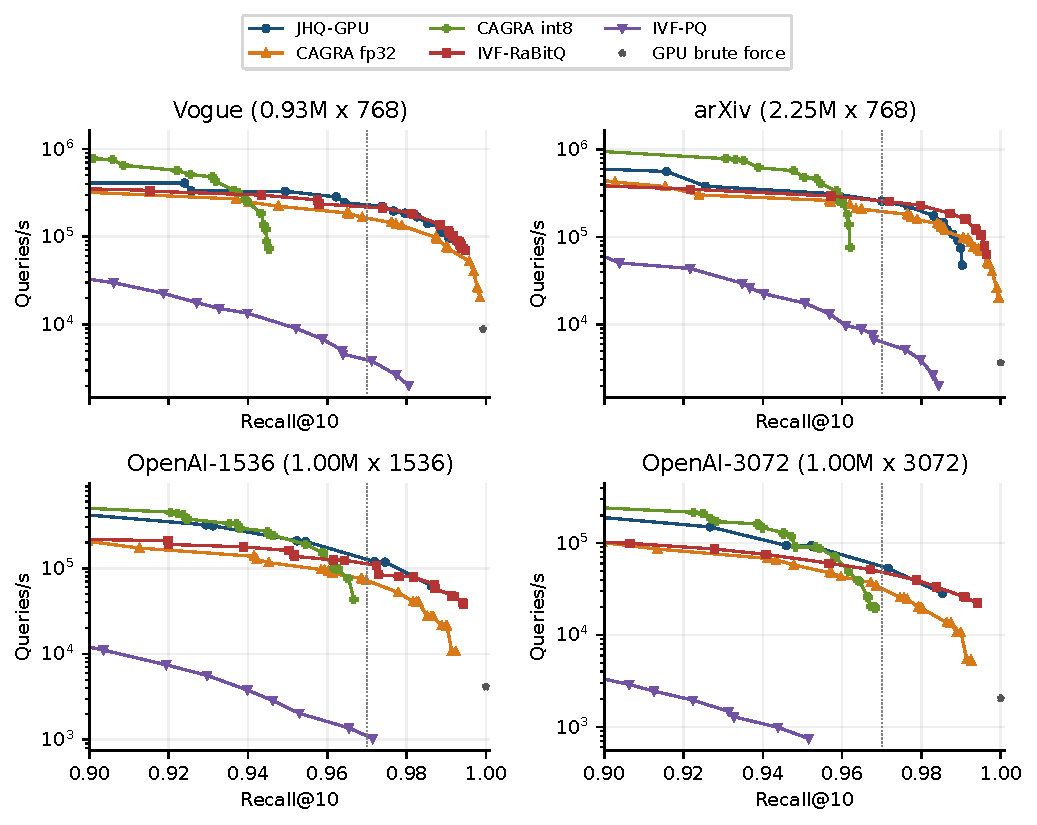
\includegraphics[width=\linewidth]{ch7/frontiers.pdf}
\caption[E1 召回率—吞吐前沿]{四个 E1 数据集上的实测主机到主机召回率—QPS 前沿。显示范围从 0.90 开始，0.97 处画垂线。包括 CAGRA int8 在内的所有基线家族均参与前沿构造。线连接实测点；吞吐轴为对数。}
\label{fig:7-frontiers}
\end{figure}

\subsection{相同召回率下的吞吐}

\Cref{tab:7-matched} 使用 \cref{sec:3-4} 定义的插值和满足阈值的实测估计器报告召回率 0.97。

\par\medskip\noindent\begin{minipage}{\linewidth}
\captionsetup{hypcap=false}
\centering
\captionof{table}[召回率 0.97 时的跨系统比较]{召回率 0.97 的比较。每个比值为“插值／实测”；大于一有利于 JHQ。JHQ kQPS 为插值估计。arXiv 与 RaBitQ 的小幅差异随估计器改变方向。}
\label{tab:7-matched}
\small\setlength{\tabcolsep}{4pt}
% Generated by scripts/build_ch7.py; do not edit numbers manually.
\begin{tabular}{@{}lrrr@{}}
\toprule
数据集 & JHQ kQPS & 相对 CAGRA fp32 & 相对 IVF-RaBitQ \\
\midrule
Vogue & 230.8 & 1.416 / 1.537 & 1.059 / 1.046 \\
arXiv & 258.6 & 1.317 / 1.422 & 0.996 / 1.015 \\
OpenAI-1536 & 126.7 & 1.747 / 2.294 & 1.130 / 1.111 \\
OpenAI-3072 & 55.9 & 1.747 / 2.088 & 1.157 / 1.346 \\
\bottomrule
\end{tabular}

\end{minipage}\par\medskip

在索引、probes、预算及最终输出固定、batch 1,000 下，去掉分组使 Vogue 在召回率 0.97 时的 JHQ／RaBitQ 比从 1.059 降至 0.933。这分离的是集成分组路径，不只是共享阈值。

CAGRA int8 在 0.90--0.92 领先 $1.20$--$1.98\times$，但不覆盖 0.97。RaBitQ 赢得部分 0.98+ 目标；CAGRA fp32 在 arXiv 接近 0.99 时领先（\cref{fig:7-frontiers}）。

\newpage
\subsection{OpenAI 数据集上的精度敏感性}
\label{sec:7-precision}

补充源码检查确定，虽然输入／存储为 FP32，且源码注释有误导，E1 实现对 OpenAI 旋转和质心 GEMM 使用 TF32 乘法与 FP32 累加（\cref{sec:4-2}）。主 E1 前沿仍是该实现的历史测量。campaign D 中，独立 FP32 变体修改 cuBLAS 运算模式开关，在 batch 1,000 下重放 37/39 个 OpenAI 配置，每个五轮。不同 probe 设置间交替变体执行顺序。两者复用同一 TF32 训练模型；干预改变 add／查询算术，包括数据库编码与路由，并非比较独立 FP32 训练的模型。\Cref{tab:7-precision} 汇总成对变化。

\par\medskip\noindent\begin{minipage}{\linewidth}
\centering\captionsetup{hypcap=false}
\captionof{table}[匹配配置下的 FP32 敏感性]{FP32 敏感性。QPS 比为相同配置下 FP32／TF32 的几何平均；召回差采用同一方向。末两列比较召回率 0.97 下的 FP32 前沿与存档 E1 IVF-RaBitQ、CAGRA fp32 前沿。campaign D 未重测基线。}
\label{tab:7-precision}
\scriptsize\setlength{\tabcolsep}{3pt}
\begin{tabular}{@{}lrrrrr@{}}
\toprule
数据集 & 配置对 & QPS 比 & $\Delta$召回 & 相对 RaBitQ & 相对 CAGRA \\
\midrule
OpenAI-1536 & 37 & 0.953 & +0.0003--+0.0005 & 1.086 & 1.679 \\
OpenAI-3072 & 39 & 0.951 & +0.0000--+0.0003 & 1.079 & 1.629 \\
\bottomrule
\end{tabular}

\end{minipage}\par\medskip

相同配置下，FP32 吞吐降低约 5\%，召回增加 0--0.0005。召回率 0.97 时，FP32 比同会话 TF32 慢约 3\%，但仍为存档 RaBitQ 的 $1.086/1.079\times$、存档 CAGRA fp32 的 $1.679/1.629\times$。新会话 v69 对存档 RaBitQ 为 1.118/1.114，历史为 1.130/1.157。D 对基线的比较跨会话；仅 v69／v72 同会话。\Cref{fig:7-precision} 展示两条 JHQ 前沿与存档对照。T1 单独重测同会话锚点，网格敏感结果见 \cref{sec:b-precision-anchors}。

\par\medskip\noindent\begin{minipage}{\linewidth}
\captionsetup{hypcap=false}
\centering
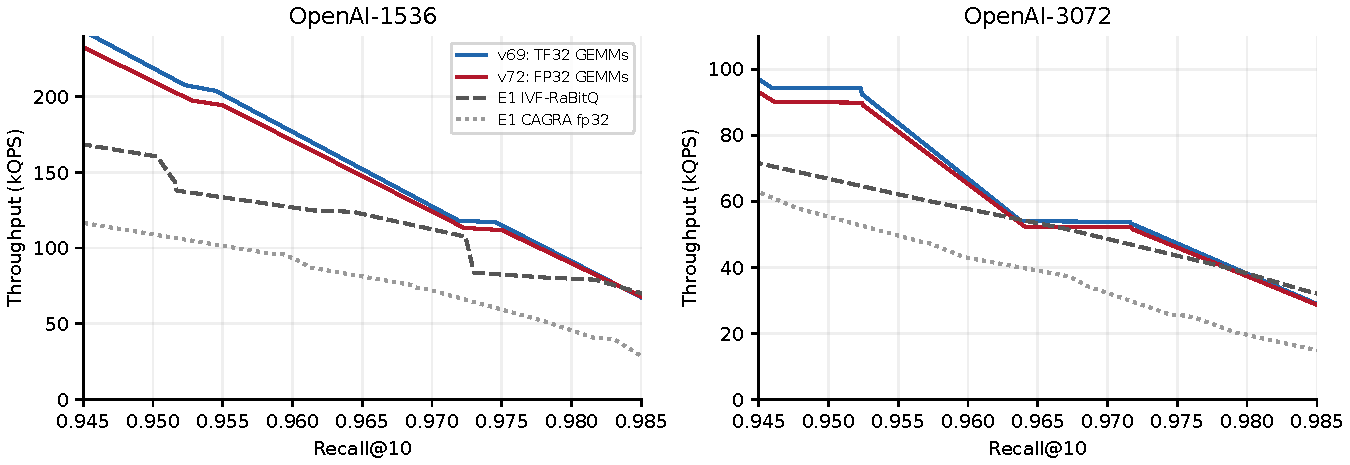
\includegraphics[width=\linewidth]{supplement/precision.pdf}
\captionof{figure}[TF32 与 FP32 精度前沿]{campaign D 的精度前沿。实线为同会话 JHQ 变体；虚线／点线基线为历史 E1 测量。均使用本章前沿与插值规则。}
\label{fig:7-precision}
\end{minipage}\par\medskip

\subsection{同会话基线比较}
\label{sec:b-precision-anchors}
T1 使用 E1 内存池，每个 OpenAI 数据集十二个成对配置。基线运行前后各有一次五轮 JHQ 重复；中位数以几何方式组合。相同配置 FP32／TF32 均值为 0.956/0.964。两者均复用 TF32 训练缓存，改变 add／查询算术。
\par\medskip\noindent\begin{minipage}{\linewidth}
\captionsetup{hypcap=false}
\centering
\captionof{table}[同会话精度锚点]{T1，召回率 0.97、batch 1,000。基线比值为插值／严格实测阈值；FP32／TF32 为插值。所有方法处于同一会话，不同于 D 的存档基线。}
\label{tab:b-precision-anchors}
\footnotesize\setlength{\tabcolsep}{3pt}
\begin{tabular}{@{}lrrr@{}}
\toprule
数据集 & FP32/TF32 at 0.97 & FP32 / RaBitQ & FP32 / CAGRA \\
\midrule
OpenAI-1536 & 0.980 & 1.126 / 1.053 & 1.752 / 1.633 \\
OpenAI-3072 & 0.973 & 1.328 / 1.316 & 1.825 / 2.019 \\
\bottomrule
\end{tabular}

\end{minipage}\par\medskip
OpenAI-3072 的 RaBitQ 括区间 0.9669--0.9796 召回体现网格敏感性。这些锚点不替代 E1，也不提供 FP32 重训练结果。


\subsection{解释与比较限制}

两个 OpenAI 数据集均使用 Qdrant DBpedia 嵌入 \cite{data_openai1536,data_openai3072}。截断／重新归一化后，1,000 个查询行与 10,299 个抽样基础行的余弦为 $\geq0.9980$，中位数 1.000000，GT 重合度 9.046/10。没有实体 ID，这些检查支持行序对齐。维度翻倍后，CAGRA 比值仍为 1.747，RaBitQ 为 1.130/1.157，因此仅凭维度无法解释。

收益伴随更小的 128-probe 预算锚点：OpenAI 为 4--8，Vogue 为 64，arXiv 为 100，后续 FULL 为 200。这是相关观察，不是独立效应，也不是匹配前沿的参数设置。

\Cref{sec:7-8} 检查小幅领先的敏感性，以及 \cref{sec:3-3} 中接口、显存和编译差异的影响。

\subsection{小 Batch 改变竞争区间}
\label{sec:7-smallbatch}

T5 在四个 E1 数据集、batch 8/32 上比较调度 JHQ、CAGRA fp32／int8 和 IVF-RaBitQ。五轮同步主机到主机测量分别使用 1,000/992 查询。1,808 个测点包含 JHQ 单 block 对照，不含 IVF-PQ／暴力搜索。\Cref{fig:7-smallbatch,tab:7-smallbatch} 比较所得区间。

\suppressfloats[t]
\par\medskip\noindent\begin{minipage}{\linewidth}
\captionsetup{hypcap=false}
\centering
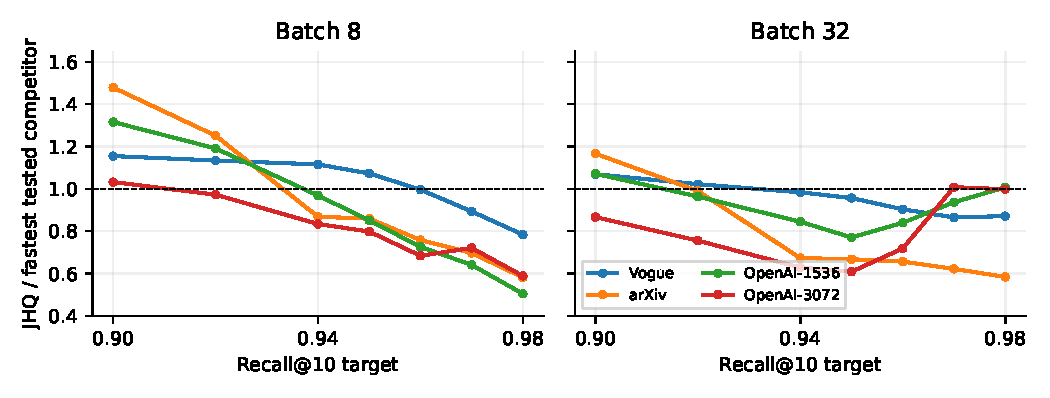
\includegraphics[width=\linewidth]{t4-t5/smallbatch.pdf}
\captionof{figure}[小 Batch 竞争区间]{T5 的 JHQ／最快对手 QPS 比，采用保留合格实测端点的插值。大于一有利于 JHQ。严格阈值见 \Cref{tab:7-smallbatch}。}
\label{fig:7-smallbatch}
\end{minipage}\par\medskip

\par\medskip\noindent\begin{minipage}{\linewidth}
\captionsetup{hypcap=false}
\centering
\captionof{table}[小 Batch 匹配召回比]{T5 QPS 比：保留合格端点的插值／严格实测阈值。各估计器独立选择最快对手；满足阈值的更高召回端点可入选，无需外推。}
\label{tab:7-smallbatch}
\footnotesize\setlength{\tabcolsep}{4pt}
\begin{tabular}{@{}lrrrr@{}}
\toprule
数据集 & $b$ & $R=0.90$ & $R=0.95$ & $R=0.97$ \\
\midrule
Vogue & 8 & 1.155 / 1.091 & 1.073 / 0.980 & 0.893 / 0.854 \\
Vogue & 32 & 1.069 / 0.997 & 0.956 / 0.895 & 0.865 / 0.839 \\
arXiv & 8 & 1.479 / 1.454 & 0.859 / 0.851 & 0.697 / 0.698 \\
arXiv & 32 & 1.166 / 1.148 & 0.667 / 0.661 & 0.622 / 0.582 \\
OpenAI-1536 & 8 & 1.316 / 1.131 & 0.851 / 0.825 & 0.641 / 0.620 \\
OpenAI-1536 & 32 & 1.071 / 0.915 & 0.770 / 0.752 & 0.937 / 0.914 \\
OpenAI-3072 & 8 & 1.032 / 0.953 & 0.798 / 0.798 & 0.721 / 0.702 \\
OpenAI-3072 & 32 & 0.866 / 0.734 & 0.608 / 0.771 & 1.008 / 1.351 \\
\bottomrule
\end{tabular}

\end{minipage}\par\medskip

batch 8／召回率 0.97 时，CAGRA fp32 在两种估计器下均赢得全部四个数据集，JHQ 比为 0.641--0.893。batch 32 时比为 0.622--1.008；实测阈值下 OpenAI-3072 有利于 JHQ。Vogue 的 batch-8／0.95 领先需要插值。网格分辨率会改变接近持平的结果。

纳入合格端点时，召回率 0.90 比值为 batch 8 的 1.032--1.479、32 的 0.866--1.166；严格实测下 JHQ 分别赢三／一个。省略端点会夸大收益。调度在 0.95 处相对单 block 提升 $1.7$--$3.3\times$，但不保证跨系统获胜。

空调用中位数为 0.012--0.072\,ms，仍计入总时间。CAGRA 使用 Python，JHQ／RaBitQ 使用 C++；预热不同（\cref{sec:a-t4-t5}）。


\section{Cartesian LUT、打包载入与 Lane 精排}
\label{sec:7-3}

RQ2 消融同时测量内核与应用效应。

\subsection{LUT 分解与吞吐}

LUT 消融测试 \cref{sec:5-2} 成本模型与 FP32 排序效应。

\Cref{fig:7-lut} 比较六个数据集上的 Cartesian 表分组，probe 数为 8/32/128/512，固定 $\alpha=100$，$\glut\in\{1,2,4,8\}$。五轮使用 batch 1,000，Stella 为 999。两组在 22/24 单元领先，例外接近持平：arXiv／128 的一组快 0.23\%，OpenAI-3072／8 的四组快 0.84\%。两组对一组成对获胜 23/24，全部数据集几何平均大于一，范围 1.021--1.318。共享索引单元并非独立试验。

\begin{figure}[!htbp]
\centering
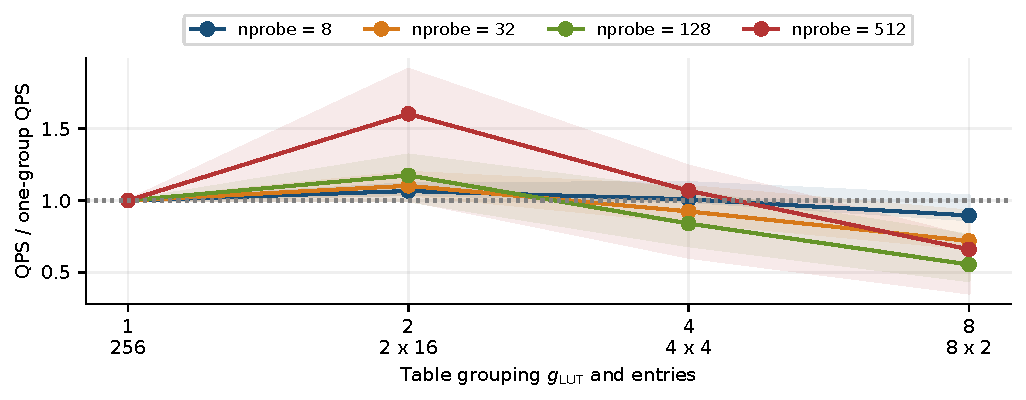
\includegraphics[width=\linewidth]{ch7/lutgroups.pdf}
\caption[Cartesian 查找表分组]{固定 $\alpha=100$ 下的 Cartesian 表分组（v71）。组数表示 $\glut$，不是并行扫描组。曲线为各数据集相对一组实验臂 QPS 比的中位数；阴影表示范围。}
\label{fig:7-lut}
\end{figure}

两组／一组比值从 $0.998$ 到 $1.914$。四组和八组均存 16 项，但需要更多查表与加法。这说明表更小不一定提高吞吐；占用率和指令成本未被单独分离。任意四臂单元中报告的最大召回差为 $10^{-4}$。128 probes、$\alpha=100$ 下，T4 在 Vogue、arXiv 和 OpenAI-3072 上比较相同候选。整表与 $16+16$ 表有 22.6--26.1\% 的候选分数 bit 模式不同，最大相对误差 $4.53\times10^{-7}$。跨全部形式，20.5--29.4\% 不同，最大相对误差 $4.64\times10^{-7}$。Vogue 有 2--4/256 个最终 ID 差异，arXiv／OpenAI 没有。主码保留集合不变时，最终 ID 仍可变化，因为舍入后的主码分数进入精排（\cref{sec:a-t4-t5}）。

\subsection{打包访问与协作残差评分}

打包在 48 对匹配配置中获胜 $1.012$--$1.658\times$，覆盖六个数据集、四个 probe 数及 $\glut\in\{1,2\}$，召回差最多 $10^{-4}$。两个布局均为 subspace-major。打包／载入／解包一起改变。每臂仅一个汇总计时，比五轮 v71 的计时证据少。

\Cref{fig:7-packing-refinement,tab:7-refinement} 进一步区分残差精排中的宽载入和 lane 协作。L0 是原始标量路径；L1 只改变载入路径，不把一个候选分到多个 lanes；L16 为每候选分配 16 lanes。同一进程在五轮计时中轮换实验臂顺序，每轮每臂三次搜索。十二个普通单元中，L16 整体提升 $1.015$--$1.789\times$；独立的高预算 arXiv／$\alpha=200$ 对照达到 $2.383\times$。

\begin{figure}[!htbp]
\centering
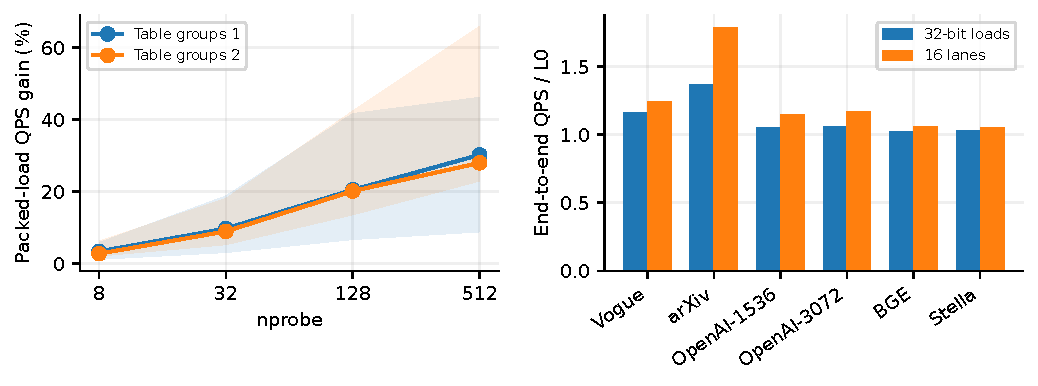
\includegraphics[width=\linewidth]{ch7/packing_refinement.pdf}
\caption[打包访问与精排对照]{打包与精排对照。左：各表分组／probe 数下，六个数据集的打包载入 QPS 收益中位数及最小—最大阴影范围。右：128 probes、各数据集普通预算下，仅改变载入和16-lane 的实测端到端收益。两个面板使用不同实验家族。}
\label{fig:7-packing-refinement}
\end{figure}

\begin{table}[!htbp]
\centering
\caption[128 probes 下的精排收益]{128 probes 下的精排。比值为相对 L0 的成对端到端收益；末列除外，它是剖析得到的精排内核收益。内核与应用收益不能互换。}
\label{tab:7-refinement}
\small\setlength{\tabcolsep}{4pt}
% Generated by scripts/build_ch7.py; do not edit numbers manually.
\begin{tabular}{@{}lrrrr@{}}
\toprule
数据集 & $\alpha$ & $L1/L0$ QPS & $L16/L0$ QPS & 内核加速 \\
\midrule
arXiv & 100 & 1.368 & 1.789 & 5.97 \\
BGE & 32 & 1.026 & 1.062 & 1.97 \\
OpenAI-1536 & 8 & 1.055 & 1.145 & 3.34 \\
OpenAI-3072 & 4 & 1.063 & 1.171 & 8.81 \\
Stella & 16 & 1.030 & 1.053 & 2.66 \\
Vogue & 64 & 1.161 & 1.240 & 3.72 \\
\bottomrule
\end{tabular}

\end{table}

仅改变载入的 L1 与 L0 逐位相同，却在 arXiv 获得 $1.368\times$。在 $\alpha=100$ 下使用 lanes，精排从 4,277.5$\to$716.8\,$\mu$s，内核提升 $5.97\times$，而整体为 $1.789\times$。OpenAI-3072 的内核／整体提升分别为 $8.81\times$／$1.171\times$。其他阶段仍存在。

基线 wall time 占比为 $f$、精排加速比为 $s$ 时，替换模型给出
\[
 \frac{T'}T=(1-f)+\frac f s,\qquad
 \frac T{T'}=\frac1{1-f+f/s}.
\]
arXiv／OpenAI-3072 的 $f=0.529/0.168$ 预测 $1.787/1.175\times$，实测为 $1.789/1.171\times$。独立剖析提供解释性估计。

Lane FP32 重新结合运算的相对距离误差达到 $\approx1.6\times10^{-6}$，偶尔改变顺序。Sanitizer 只覆盖记录的子集，未声称普遍逐位相同。

\section{选择正确性与性能}
\label{sec:7-4}

\subsection{计算分数选择的严格 CPU 参考}
\label{sec:7-strict-selection}

全部 55,296 个分组查询实例的主码顺序与 CPU 参考精确一致。单 block 始终满足距离顺序，56 个集合差异均限于截断并列；全部 69,120 个实例对已保留精排分数的最终选择均精确（\cref{tab:7-strict-selection}）。

严格 CPU 检查对 GPU 生成的分数按 $(\primarydist,\mathrm{position})$ 排序。导出器遵循扫描布局和累加顺序，有效返回候选的导出分数逐位匹配。源码比较发现相对表扫描版本只增加导出。270 个配置覆盖 Vogue、arXiv 和 OpenAI-3072，probes 为 1、8、128，$\alpha\in\{4,100,200\}$、$\gscan\in\{0,1,2,4,8\}$ 以及两种阈值设置。

\suppressfloats[t]
\begin{table}[!htbp]
\centering
\caption[严格计算分数选择检查]{严格选择检查 CPU 参考检查。集合与顺序相等使用完整主码键。有效计数检查 $\min(c,n_c)$ 个保留候选；最终相等按 $(\refineddist,\mathrm{ID})$ 对保留的计算精排分数排序，包含其 FP32 bits。计数为查询实例，同一查询跨配置复用。}
\label{tab:7-strict-selection}
\footnotesize\setlength{\tabcolsep}{3pt}
\begin{tabular}{@{}lrrrrr@{}}
\toprule
路径 & 查询数 & 集合／顺序精确 & 仅并列 & 有效计数 & 最终精确 \\
\midrule
$\gscan\geq1$ & 55,296 & 55,296 / 55,296 & 0 & 55,296 & 55,296 \\
$\gscan=0$ & 13,824 & 13,768 / 8,758 & 56 & 13,824 & 13,824 \\
\bottomrule
\end{tabular}

\end{table}

全部 19,120 个候选不足案例的有效候选数正确。这些结果检验了 \cref{lem:5-buffer,prop:5-local-coverage,prop:5-shared-bound} 在记录案例中的表现。最终选择相等针对已保留的计算分数，而非原始空间精确近邻；sanitizer 覆盖限于其记录子集（\cref{sec:a-t4-t5}）。


\subsection{共享阈值保持选择目标}

48 组输出全部一致，QPS 比为 $0.994$--$1.562\times$。在 arXiv $\alpha=200$、batch 1,000、八组下，共享使归并从 2,629$\to$471\,$\mu$s，扫描从 7,968$\to$5,513\,$\mu$s。部分单元略有退步。

试验第一组包含 46--81\% 的优胜者。相同配额需要回退，不同配额仍留有瓶颈。阈值避免固定配额。

\subsection{探测列表选择与输出一致性}

Radix 保持评分算术／OpenAI TF32（\cref{sec:7-precision}）。全部 1,792 个合成用例通过。对 arXiv／Vogue／OpenAI-3072 的全部 1,000 个查询，probes 以及主码分数／位置均匹配。

\par\medskip\noindent\begin{minipage}{\linewidth}
\captionsetup{hypcap=false}
\centering
\captionof{table}[Probe 选择吞吐比]{精确计算分数 probe 改动的 v69／v65 端到端吞吐比。每个工作负载—batch 比较中，每个二进制有十轮计时，交替运行收集。$>1$ 的比值有利于 v69。}
\label{tab:7-probe}
\small
% Generated by scripts/build_ch7.py; do not edit numbers manually.
\begin{tabular}{@{}lrrrr@{}}
\toprule
数据集 & Batch 8 & 32 & 256 & 1,000 \\
\midrule
arXiv & 1.074 & 1.063 & 1.035 & 1.034 \\
Vogue & 1.109 & 1.103 & 1.052 & 1.041 \\
OpenAI-3072 & 1.167 & 1.117 & 1.055 & 1.050 \\
\bottomrule
\end{tabular}

\end{minipage}\par\medskip

\Cref{tab:7-probe} 显示端到端提升 $1.034$--$1.167\times$。batch 8 下，剖析的 probe 阶段在 arXiv 从 56.5 降至 22.6\,$\mu$s，Vogue 从 52.7 降至 14.7\,$\mu$s，OpenAI-3072 从 77.8 降至 16.7\,$\mu$s。未改阶段限制全 batch 收益，各比值使用自己的基线。

Vogue 在跨二进制的 1,000 查询转储中，probe／主码逐字节一致（一组／batch-8），最终召回却为 0.9642/0.9644。基线自身在一致性／计时运行间也由 0.9642 变为 0.9644。本次检查中，变化发生在主码选择之后，原因未解决。同进程内调度／单 block 输出匹配（\cref{app:reproducibility}）。

可选 FP16 probe 集合在 arXiv／Vogue／OpenAI-3072 的 1,000 查询中分别有 936/979/998 个与 v69 一致。高度重合不等于精确。这些结果不纳入主 E1 前沿，也不纳入精确 probe 主张。

\section{留出预算质量、吞吐与回本}
\label{sec:7-5}

RQ3 将 \cref{ch:refinement} 的策略与固定 $\alpha=100$ 及更强的通用对照 $\alpha=64$ 比较。

\subsection{无标签选择与有标签诊断 Oracle}

六个数据集在 128、512 probes 下测试 \cref{sec:6-4} 的固定、抽样、FULL、枚举和 oracle 对照。不相交查询池及每样本量 64 次抽样遵循 \cref{sec:3-2}。

所有规则变体均使用 \cref{eq:6-agreement}，取 $k=10$、$\epsilon=1$。FULL 使用全部校准查询；诊断 oracle 使用留出标签（\cref{tab:6-controls}）。

\subsection{全池校准作为质量优先工作点}

每个单元对全部 500 个校准查询执行一次全池校准。所选实验臂在 12/12 单元满足留出 $10^{-3}$ 损失目标，最大观测损失为 0.0006。其速率为 GT oracle 的 0.908--1.000，校准成本 9.5--60.3\,ms。相对固定 100 的速率几何平均比为 $1.111\times$；只看固定 100 也达标的十个单元，则为 $1.193\times$。\Cref{tab:7-budget-full} 给出完整比较。相对固定 64，全池选择在六个单元更快、两个持平、四个更慢；主要优势是观测中覆盖了全部十二个质量目标。

这些单元支持质量优先时用 FULL，校准成本优先时用 $S=128$（\cref{sec:6-2}）。

\begin{table}[!htbp]
\centering
\caption[全池预算校准]{全池校准（$S=500$）。损失相对最佳实测留出召回率；速率为所选固定臂的 kQPS。“Cal.”是每单元一次全池校准调用，不是重复查询流计时。留出查询为 500 个，Stella 为 499 个。}
\label{tab:7-budget-full}
\footnotesize\setlength{\tabcolsep}{3pt}
% Generated by scripts/build_ch7.py; do not edit numbers manually.
\begin{tabular}{@{}lrrrrrrr@{}}
\toprule
数据集 & Probe & $\alpha_{\rm full}$ & 损失 & $Q_{\rm full}$ & 相对 100 & 相对 oracle & 校准 ms \\
\midrule
Vogue & 128 & 100 & 0.0000 & 202.9 & 1.000 & 0.908 & 10.1 \\
arXiv & 128 & 200 & 0.0000 & 151.5 & 0.728 & 1.000 & 10.0 \\
OpenAI-1536 & 128 & 8 & 0.0000 & 267.7 & 1.599 & 1.000 & 9.5 \\
OpenAI-3072 & 128 & 4 & 0.0000 & 145.0 & 1.691 & 1.000 & 17.1 \\
BGE & 128 & 64 & 0.0006 & 124.9 & 1.075 & 0.932 & 17.1 \\
Stella & 128 & 16 & 0.0006 & 110.4 & 1.153 & 1.000 & 20.6 \\
Vogue & 512 & 100 & 0.0002 & 100.1 & 1.000 & 0.969 & 20.9 \\
arXiv & 512 & 200 & 0.0000 & 69.0 & 0.831 & 1.000 & 25.1 \\
OpenAI-1536 & 512 & 8 & 0.0000 & 114.9 & 1.326 & 1.000 & 21.8 \\
OpenAI-3072 & 512 & 4 & 0.0002 & 52.1 & 1.219 & 0.977 & 40.5 \\
BGE & 512 & 64 & 0.0006 & 50.8 & 1.033 & 1.000 & 42.3 \\
Stella & 512 & 16 & 0.0006 & 36.0 & 1.041 & 1.000 & 60.3 \\
\bottomrule
\end{tabular}

\end{table}

\subsection{低成本抽样及其质量风险}

\Cref{tab:7-budget-quality} 报告 $S=128$ 结果。十二个单元中，十个所选预算中位数匹配 oracle；arXiv／128 probes 和 OpenAI-3072／512 不同。预算跨工作负载为 4--200。预算中位数与平均召回不一定对应同一实验臂。平均召回由打印的最佳召回减去平均损失重建，约保留四位小数。

\begin{table}[!htbp]
\centering
\caption[抽样预算的留出质量]{$S=128$ 下的留出质量。规则 $\alpha$ 为 64 次抽样中位数；oracle $\alpha$ 使用留出标签。$\overline R_{\rm rule}$ 为重建的平均召回。“Losses”计数相对最佳已测留出召回损失 $>10^{-3}$ 的抽样次数；$L_{95}$ 为日志中的较低次序 95 分位损失估计。$R_{100}$ 为固定预算召回。}
\label{tab:7-budget-quality}
\small\setlength{\tabcolsep}{3pt}
% Generated by scripts/build_ch7.py; do not edit numbers manually.
\begin{tabular}{@{}lrrrrrr@{}}
\toprule
数据集 & Probe & $\alpha$: 规则/oracle & $R_{100}$ & $\overline{R}_{\rm rule}$ & 越阈数 & $L_{95}$ \\
\midrule
Vogue & 128 & 64 / 64 & 0.9680 & 0.9677 & 5/64 & 0.0022 \\
arXiv & 128 & 100 / 200 & 0.9748 & 0.9751 & 40/64 & 0.0024 \\
OpenAI-1536 & 128 & 8 / 8 & 0.9280 & 0.9279 & 4/64 & 0.0000 \\
OpenAI-3072 & 128 & 4 / 4 & 0.9252 & 0.9252 & 0/64 & 0.0000 \\
BGE & 128 & 32 / 32 & 0.9198 & 0.9190 & 1/64 & 0.0008 \\
Stella & 128 & 16 / 16 & 0.9892 & 0.9884 & 6/64 & 0.0030 \\
Vogue & 512 & 64 / 64 & 0.9916 & 0.9915 & 2/64 & 0.0002 \\
arXiv & 512 & 200 / 200 & 0.9878 & 0.9885 & 32/64 & 0.0016 \\
OpenAI-1536 & 512 & 8 / 8 & 0.9740 & 0.9738 & 4/64 & 0.0000 \\
OpenAI-3072 & 512 & 4 / 8 & 0.9704 & 0.9702 & 0/64 & 0.0002 \\
BGE & 512 & 64 / 64 & 0.9670 & 0.9661 & 24/64 & 0.0014 \\
Stella & 512 & 16 / 16 & 0.9954 & 0.9945 & 7/64 & 0.0030 \\
\bottomrule
\end{tabular}

\end{table}

arXiv 在 128/512 probes 下分别有 40/64、32/64 次损失越阈，尽管平均损失只有 0.0009。固定 100 损失 0.0012/0.0016：比默认更好未必达标。BGE／512 有 24 次越阈且 $L_{95}=0.0014$；Stella 达到 0.0030；OpenAI-3072 没有越阈（\cref{tab:7-budget-quality}）。四次损失可与报告 $L_{95}=0$ 同时出现（\cref{sec:a-budget-contract}）。

\begin{figure}[!htbp]
\centering
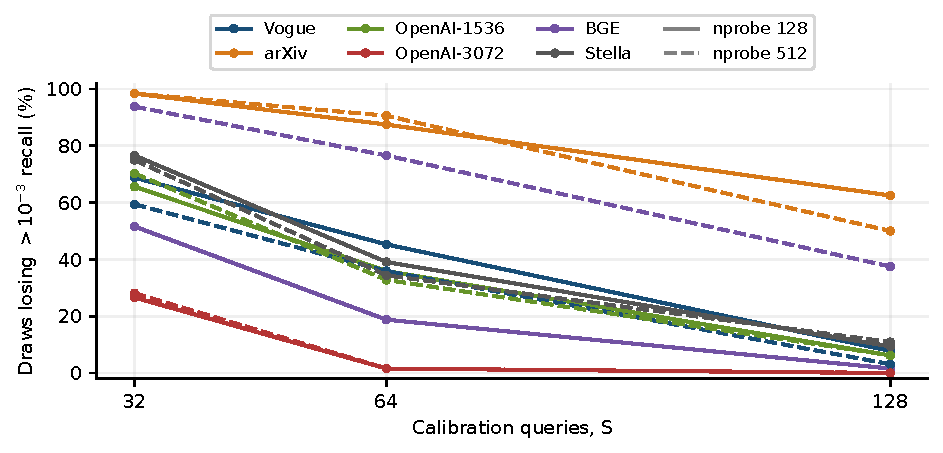
\includegraphics[width=0.82\linewidth]{ch7/budget_risk.pdf}
\caption[不同样本量下的留出风险]{不同样本量下的留出风险。纵轴为相对最佳已测预算，留出召回损失超过 $10^{-3}$ 的校准抽样百分比。因为 \cref{eq:6-agreement} 保持阈值为一，增加 $S$ 也会收紧允许的槽位不一致比例。}
\label{fig:7-budget-risk}
\end{figure}

\subsection{吞吐估计与校准经济性}

按 \cref{sec:a-budget-contract} 的平均所选臂估计，$S=128$ 在十个单元超过固定 100，幅度 $1.028$--$1.691\times$。arXiv 为 0.908/0.917，但平均召回更好，没有吞吐回本。

相对固定 64，抽样赢得 9/12 单元：几何平均 $1.054\times$，范围 $0.821$--$1.367\times$，OpenAI 为 $1.052$--$1.367\times$。两个固定对照均未满足 arXiv 质量，无法作统一质量匹配比较。

\begin{table}[!htbp]
\centering
\caption[抽样校准经济性]{$S=128$ 下的校准经济性。速率单位为 kQPS；规则速率是平均所选臂 QPS。比值分别比较固定 100 和 64。“Batches”用 500 查询、Stella 为 499，给出相对固定 100 的回本次数；“Never”表示无吞吐回本。质量列单独标明固定 100 是否满足留出损失目标。}
\label{tab:7-budget-cost}
\footnotesize\setlength{\tabcolsep}{3pt}
% Generated by scripts/build_ch7.py; do not edit numbers manually.
\begin{tabular}{@{}lrrrrrrrr@{}}
\toprule
数据集 & Probe & $Q_{100}$ & $\overline Q_{\rm rule}$ & 相对 100 & 相对 64 & 校准 ms & 批次数 & \shortstack{固定 100\\质量} \\
\midrule
Vogue & 128 & 202.9 & 224.4 & 1.106 & 1.004 & 4.0 & 17.0 & 达标 \\
arXiv & 128 & 207.9 & 188.8 & 0.908 & 0.821 & 4.2 & 不回本 & 未达标 \\
OpenAI-1536 & 128 & 167.5 & 268.5 & 1.603 & 1.367 & 3.9 & 3.5 & 达标 \\
OpenAI-3072 & 128 & 85.7 & 145.0 & 1.691 & 1.230 & 5.7 & 2.4 & 达标 \\
BGE & 128 & 116.2 & 131.2 & 1.130 & 1.051 & 6.5 & 13.2 & 达标 \\
Stella & 128 & 95.7 & 110.3 & 1.153 & 1.087 & 7.5 & 10.8 & 达标 \\
Vogue & 512 & 100.1 & 102.9 & 1.028 & 0.996 & 7.5 & 55.4 & 达标 \\
arXiv & 512 & 83.1 & 76.2 & 0.917 & 0.870 & 9.7 & 不回本 & 未达标 \\
OpenAI-1536 & 512 & 86.6 & 115.0 & 1.327 & 1.268 & 8.8 & 6.2 & 达标 \\
OpenAI-3072 & 512 & 42.8 & 52.1 & 1.219 & 1.052 & 13.1 & 6.2 & 达标 \\
BGE & 512 & 49.2 & 51.1 & 1.039 & 1.006 & 15.8 & 41.2 & 达标 \\
Stella & 512 & 34.6 & 36.0 & 1.041 & 1.028 & 21.3 & 37.1 & 达标 \\
\bottomrule
\end{tabular}

\end{table}

校准成本 3.9--21.3\,ms。相对固定 100/64，最大正收益预计回本时间为 0.54/2.72\,s，FULL 为 1.52/2.25\,s（\cref{sec:6-5,eq:6-payback,tab:7-budget-cost}）。arXiv 固定对照质量不达标；下面的直接复用同时测成本和召回。

\subsection{完整决策轨迹与有限池风险}
\label{sec:7-budget-trace}

全部 2,304 条抽样曲线和十二条 FULL 曲线均单调，选择与枚举一致。记录的子集和复现 18,432 个网格计数（\cref{eq:6-finite-pool}）。这验证已记录汇总；任意子集／位置不变性及一般的仅距离嵌套仍有条件（\cref{sec:6-3}）。

$S=128$ 下最大损失为 arXiv／512 的 0.0050、BGE／512 的 0.0046，$S=32$ 下为 0.0294。FULL 保持在 0.0006 内。

arXiv／128 在 $S=32/64/128$ 下预测／观测越阈分别为 0.965/0.984、0.875/0.875、0.620/0.625（\cref{fig:7-finite-pool}）。36 个差距中最大为 BGE／512 的 0.144，即 0.519/0.375。GT 损失预测需要稳定计数／留出臂质量；校准本身不使用标签。

\begin{figure}[!htbp]
\centering
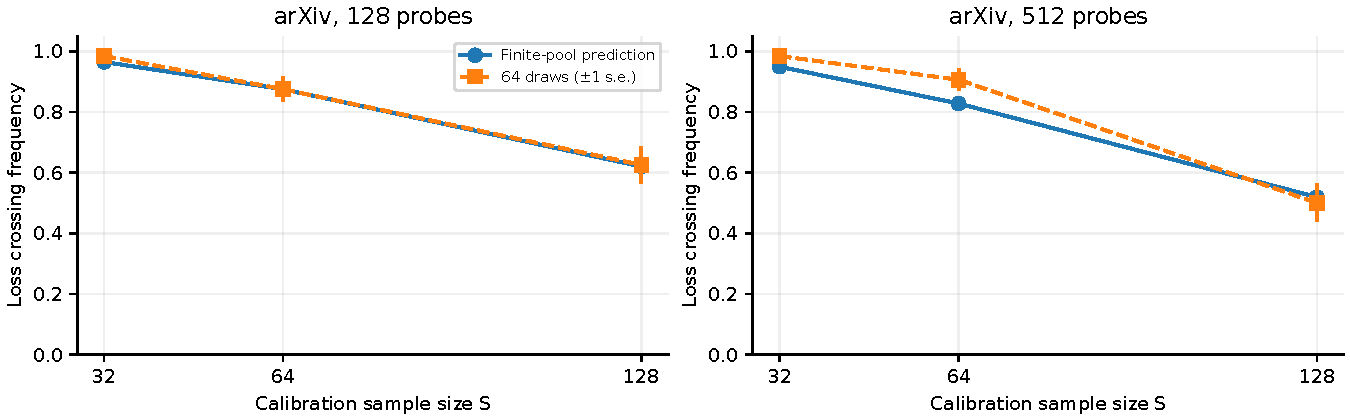
\includegraphics[width=\linewidth]{supplement/finite-pool.pdf}
\caption[有限池风险预测与观测]{有限池预测与观测到的 arXiv 损失越阈。误差条为固定池条件下 64 个独立抽样子集的一倍估计标准误，不表示未来工作负载的不确定性。}
\label{fig:7-finite-pool}
\end{figure}

十次交替重复支持低预算计时平台，而非一般运行时间单调性。

\subsection{直接测量校准加复用}
\label{sec:7-stream-cost}

四个单元在五轮轮换顺序中，对 500 个重复留出 batches 比较固定 64/100、抽样和 FULL。计时包含查询收集、校准、预算应用和首次图，不含构建、预热及扫描校准（\cref{tab:7-stream-cost}）。

\par\medskip\noindent\begin{minipage}{\linewidth}
\centering\captionsetup{hypcap=false}
\captionof{table}[500 个复用 Batch 的直接成本]{500 个复用 batches 的直接总毫秒数，取五轮平均，抽样与 FULL 策略包含预算校准。每 batch 有 500 查询。质量与计时结果一同讨论。}
\label{tab:7-stream-cost}
\footnotesize\setlength{\tabcolsep}{4pt}
\begin{tabular}{@{}lrrrr@{}}
\toprule
数据集／probes & 固定 100 & 固定 64 & 规则 $S=128$ & FULL \\
\midrule
arXiv/128 & 1224 & 1102 & 1291 & 1680 \\
OpenAI-1536/128 & 1491 & 1264 & 852 & 860 \\
OpenAI-3072/128 & 2757 & 2160 & 1769 & 1783 \\
BGE/512 & 5185 & 5018 & 4921 & 5062 \\
\bottomrule
\end{tabular}

\end{minipage}\par\medskip

OpenAI-3072 两种策略均选 4，召回 0.9252，与固定 100 相同。OpenAI-1536 的 FULL／固定 100 为 0.9280，抽样为 0.9276。时间见 \Cref{tab:7-stream-cost}。

相对固定 100/64，直接节省分别从 OpenAI-1536 的 4/6 个 batches、OpenAI-3072 的 4/9 个 batches 开始（\cref{fig:7-stream-cost}）；分数批次拟合结果有所不同。BGE 抽样／固定 100／FULL 召回为 0.9658/0.9670/0.9664。arXiv FULL 为质量选择更慢的 200，固定对照不达标。

\par\medskip\noindent\begin{minipage}{\linewidth}
\captionsetup{hypcap=false}
\centering
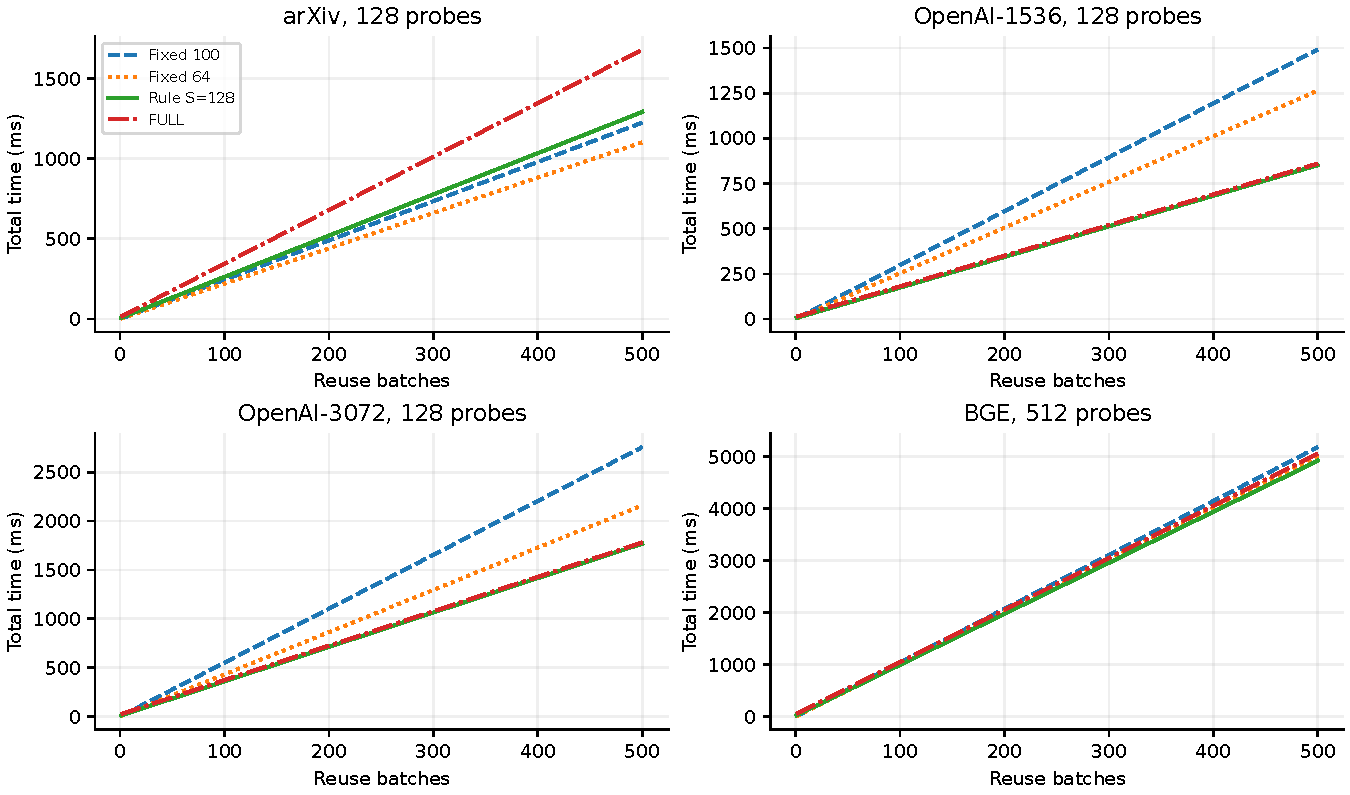
\includegraphics[width=\linewidth]{supplement/stream-cost.pdf}
\captionof{figure}[校准后复用的直接累计时间]{直接测得的平均累计时间，包含预算校准和首 batch 准备。每条曲线重放一个固定留出查询池。不同策略可能有不同召回率；仅靠时间不能形成质量匹配排名。数据集／probe 设置与 \cref{tab:7-stream-cost} 相同。}
\label{fig:7-stream-cost}
\end{minipage}\par\medskip


\section{批量大小、调度与负载不均}
\label{sec:7-6}

\subsection{并行度与重复选择工作}

batch-8 的八组提升 $2.06$--$2.76\times$；arXiv 扫描从 849$\to$216\,$\mu$s，另加 16.7\,$\mu$s 归并。batch 1,000、$\alpha=200$ 时，独立分组反而将扫描从 3,530$\to$7,652\,$\mu$s，另加 2,624\,$\mu$s 归并，仅达到单 block QPS 的 $0.46\times$。共享阈值减少工作，但未消除区间变化。

\begin{figure}[!htbp]
\centering
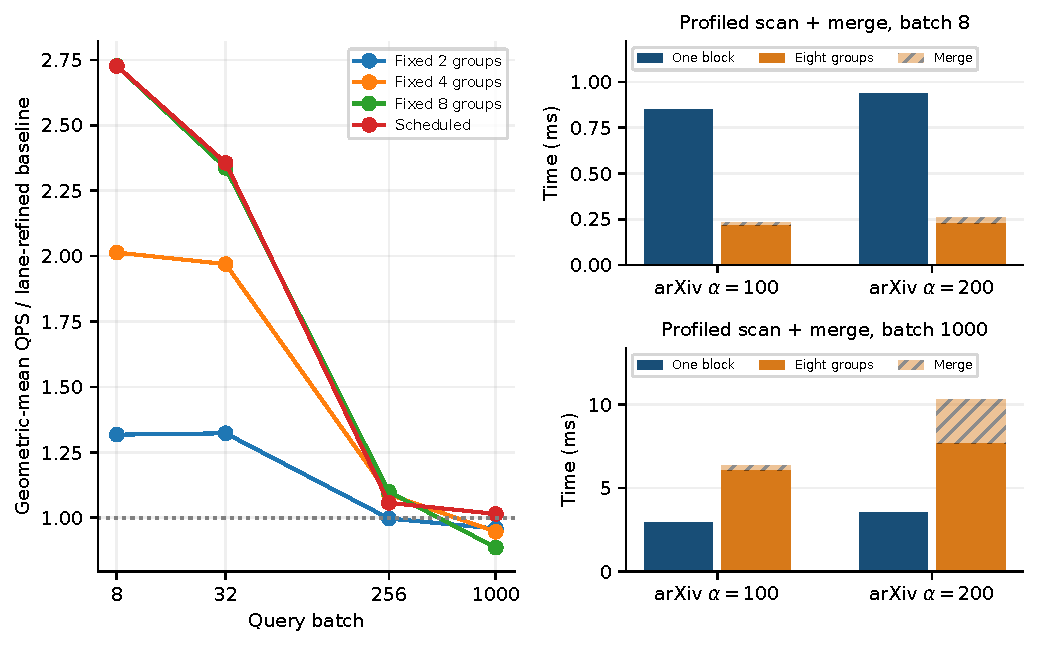
\includegraphics[width=\linewidth]{ch7/batch_execution.pdf}
\caption[依赖 Batch 的执行区间]{执行区间。左：固定共享阈值组数及调度执行，相对 lane 精排单 block 基线的速率；小 batch 有 13 单元，batch 1,000 有 11。右：arXiv 预算 100、200 在 batch 8、1,000 下的成对扫描／归并剖析。斜纹表示归并。右侧来自独立阈值扫描实验，解释一种成本，不是调度器的完整加速。}
\label{fig:7-batch}
\end{figure}

\subsection{在更多配置上评估固定规则}

调度遵循 \cref{sec:5-5} 的填充／偏斜规则与伪查询校准。四个配置先确定常数，再测量其他配置。

\begin{table}[!htbp]
\centering
\caption[集成执行与调度收益]{相对 v61 L16 的集成执行收益。条目为五轮逐单元成对加速比中位数的几何平均。“Held out”排除确定规则的四个配置，表示留出配置，而非预算实验的留出查询划分。}
\label{tab:7-scheduling}
\small\setlength{\tabcolsep}{4pt}
% Generated by scripts/build_ch7.py; do not edit numbers manually.
\begin{tabular}{@{}rrrrrrr@{}}
\toprule
Batch & 单元数 & $g_s=2$ & $g_s=4$ & $g_s=8$ & 调度 & 留出配置 \\
\midrule
8 & 13 & 1.318 & 2.014 & 2.728 & 2.727 & 2.930 \\
32 & 13 & 1.323 & 1.970 & 2.337 & 2.356 & 2.560 \\
256 & 13 & 0.997 & 1.090 & 1.099 & 1.057 & 1.041 \\
1000 & 11 & 0.959 & 0.947 & 0.886 & 1.015 & 1.012 \\
\bottomrule
\end{tabular}

\end{table}

平均值使用十三个小 batch 配置、十一个全 batch 配置；Stella 有 999 查询。留出子集分别为九／七个（\cref{tab:7-scheduling}）。batch 1,000 下，八组为 $0.886\times$；最坏 regret 为 1.217（BGE／256）。

Vogue 的 CV 0.338--0.622 在 batch 1,000 时选择四组。比值范围 0.895--1.175；$(n_{\rm probe},\alpha)=(16,16),(16,64),(32,64)$ 对应 0.955、0.895、0.955。CV 测量离散程度，而非总工作量：它使 0.97 处领先，却在低 probe 负载上过度分组（\cref{sec:7-2}）。

250 个变体／配置对、234,320 次查询比较中，没有非并列主码差异或最终 ID 集合差异。并列输出顺序可能不同。这些是顺序同步吞吐测试，不是开放到达流尾延迟测试。

\section{冷构建、常驻显存与已测规模}
\label{sec:7-7}

冷构建、常驻显存和完成的大数据集搜索用于评估 RQ1；E1 显存比较也支持 RQ4。

\subsection{冷构建与生命周期边界}

三次空缓存重复得到 Vogue 训练 298--303\,ms，总计 $\approx0.56$\,s，而较慢存档为 1.33\,s。Stella 为 10.54--10.65\,s，存档为 10.40\,s（\cref{tab:7-build-memory}）。

\begin{table}[!htbp]
\centering
\caption[冷构建与常驻显存]{冷 JHQ 构建与单独测量的常驻显存。Train／add 为三次补充正常构建的组件中位数；Total 为成对总和中位数。显存来自 v71 的两组、128 probes、$\alpha=100$ 运行，包含上下文和工作区。“Residual”是残差编码模型大小占实测使用总量的比例，不是每查询读取比例。}
\label{tab:7-build-memory}
\small\setlength{\tabcolsep}{3pt}
% Generated by scripts/build_ch7.py; do not edit numbers manually.
\begin{tabular}{@{}lrrrrrr@{}}
\toprule
数据集 & 训练 s & Add s & 合计 s & 使用 GiB & 原始 GiB & 残差占比 \\
\midrule
Vogue & 0.30 & 0.26 & 0.56 & 1.47 & 2.67 & 45.4\% \\
arXiv & 0.48 & 0.51 & 0.99 & 2.58 & 6.45 & 62.5\% \\
OpenAI-1536 & 0.61 & 0.38 & 1.00 & 2.39 & 5.72 & 59.7\% \\
OpenAI-3072 & 1.16 & 0.67 & 1.82 & 4.14 & 11.43 & 69.0\% \\
BGE & 3.56 & 3.65 & 7.20 & 11.93 & 38.50 & 80.7\% \\
Stella & 3.55 & 6.99 & 10.55 & 20.44 & 67.81 & 82.9\% \\
\bottomrule
\end{tabular}

\end{table}

\Cref{sec:3-3,sec:a-e1-protocol} 定义启动／构建边界；\cref{fig:7-build} 比较重复构建。

\par\medskip\noindent\begin{minipage}{\linewidth}
\captionsetup{hypcap=false}
\centering
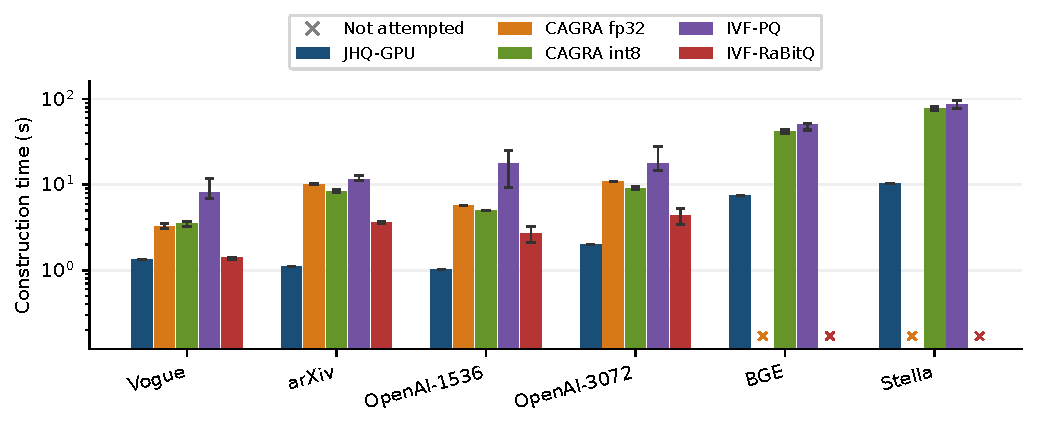
\includegraphics[width=\linewidth]{ch7/construction.pdf}
\captionof{figure}[记录的构建成本]{记录的构建成本，纳入 CAGRA int8。JHQ 为输入页已热时三次补充正常冷构建的中位数及范围；其他柱为成功测量索引配置的中位数，误差线为最小—最大值。Int8 包含数据集量化；RaBitQ 不含所需序列化往返。缺失大数据集柱表示未尝试，不是实测构建失败。纵轴为对数。}
\label{fig:7-build}
\end{minipage}\par\medskip

Stella 的隔离 CAGRA int8 为 74.55/82.45\,s，含量化；三个 IVF-PQ 配置的中位数为 86.59\,s，而 JHQ 为 10.54--10.65\,s。质量／常驻显存另行比较。

五次 arXiv 构建的召回范围为 0.0012。Stella 启动在热页下为 18.2--18.6\,s，首次读取为 129.9\,s。20\,ms 采样峰值为 BGE 26.08\,GiB、Stella 22.58\,GiB。BGE 的 12\,GiB 分配缓冲先于 23.05\,GiB gather 载荷存活，不能相加（\cref{eq:4-assignment-scratch}）。

\subsection{常驻分配与压缩的作用}

\Cref{fig:7-memory} 将 \cref{sec:4-4} 组件模型与实测常驻总量结合，保留未归属余量。前述构建测量给出采样峰值。

\par\medskip\noindent\begin{minipage}{\linewidth}
\captionsetup{hypcap=false}
\centering
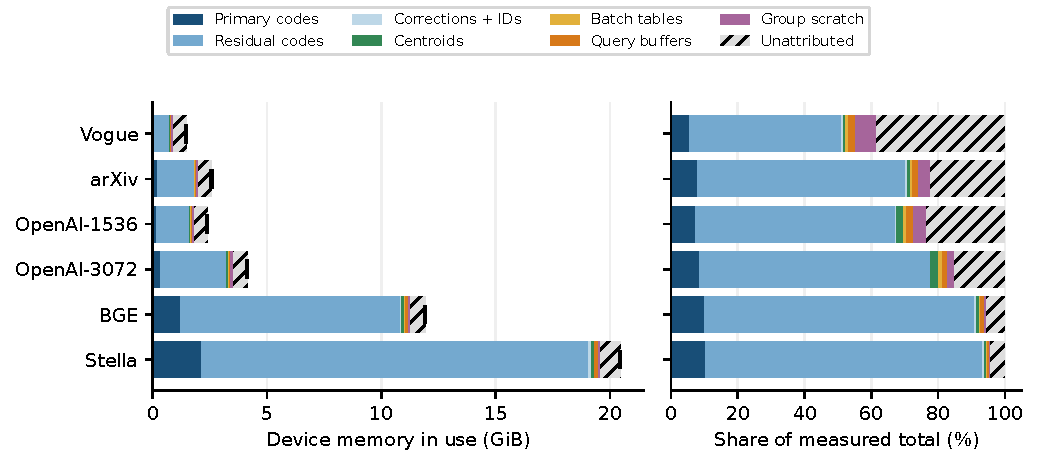
\includegraphics[width=\linewidth]{ch7/memory.pdf}
\captionof{figure}[常驻显存分解]{两组表、128 probes、$\alpha=100$ 下的常驻显存分解。组件大小为模型值，标记为实测使用总量，斜纹为未归属余量。总量包含上下文和工作区。前述构建测量给出采样峰值；这些常驻标记不是峰值。}
\label{fig:7-memory}
\end{minipage}\par\medskip

残差占 BGE 11.93\,GiB 总量的 80.7\%，占 Stella 20.44\,GiB 的 82.9\%，总量含上下文／工作区。原向量需要 38.50/67.81\,GiB。更小 $\alpha$ 节省读取，不减少存储残差 bytes（\cref{sec:4-4}）。

E1 测量在 \cref{tab:7-e1-memory} 提供独立跨系统视角。从 JHQ 进程总量减去基线测得的 507.2\,MiB 上下文，约为 CAGRA fp32 索引分配的 0.29--0.39。JHQ 包含工作区，CAGRA 则为构建时索引增量。这些是参数扫描范围，不是显存匹配召回点或等峰值预算比较。同表 CAGRA int8 与 JHQ 分配同量级：相对 fp32 的压缩并非 JHQ 独有。\cref{tab:4-bytes} 组件模型解释这一比较。

\par\medskip\noindent\begin{minipage}{\linewidth}
\captionsetup{hypcap=false}
\centering
\captionof{table}[E1 分配范围]{E1 分配范围。JHQ 为进程总量减去估计的 507.2\,MiB 上下文，包含查询工作区；两个 CAGRA 列是构建时测得的索引分配。范围覆盖参数扫描。}
\label{tab:7-e1-memory}
\footnotesize\setlength{\tabcolsep}{4pt}
% Generated by scripts/build_ch7.py; do not edit numbers manually.
\begin{tabular}{@{}lrrr@{}}
\toprule
数据集 & \shortstack{JHQ 净值\\进程 GiB} & \shortstack{CAGRA fp32\\索引 GiB} & \shortstack{CAGRA int8\\索引 GiB} \\
\midrule
Vogue & 0.90--1.01 & 2.89--2.91 & 0.89--0.91 \\
arXiv & 2.01--2.19 & 6.84--6.98 & 2.01--2.15 \\
OpenAI-1536 & 1.79--2.33 & 5.95--5.97 & 1.67--1.68 \\
OpenAI-3072 & 3.54--3.82 & 11.67--11.68 & 3.10--3.11 \\
\bottomrule
\end{tabular}

\end{minipage}\par\medskip

\subsection{大数据集可行性与竞争区间}

BGE 包含 10,091,524 个向量，Stella 为 17,776,615；二者均为 1,024 维、32,768 个 IVF 列表。Stella 查询从语料中抽取，因此结果刻画这一基准，不是独立采集的外部查询分布。\Cref{fig:7-large} 纳入成功的 CAGRA int8 与 IVF-PQ 测量。预计存储超容量时，完整精度 CAGRA／RaBitQ／FP32 暴力搜索被预先排除。这是计划排除，不是实测 OOM 或召回失败。

\par\medskip\noindent\begin{minipage}{\linewidth}
\captionsetup{hypcap=false}
\centering
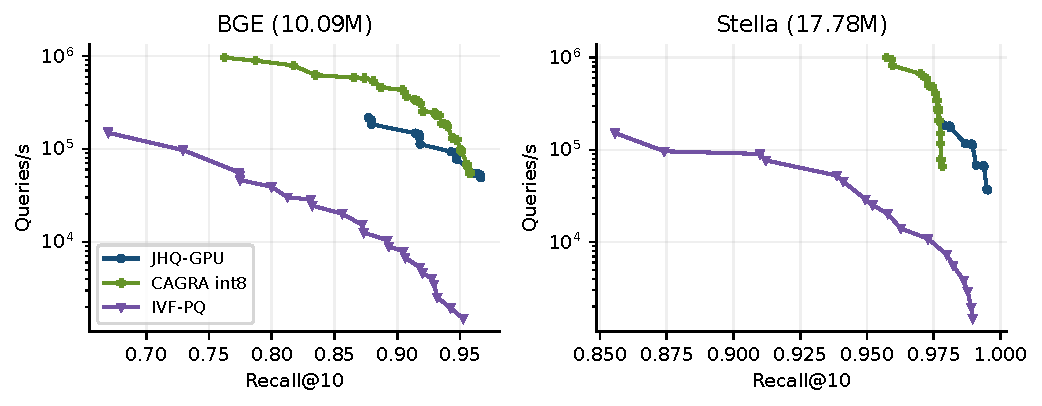
\includegraphics[width=\linewidth]{ch7/large_frontiers.pdf}
\captionof{figure}[大数据集搜索前沿]{大数据集主机到主机前沿，纳入成功的隔离 CAGRA int8 重跑。BGE／Stella 使用 1,000/999 查询。端点标记已测网格覆盖。}
\label{fig:7-large}
\end{minipage}\par\medskip

CAGRA int8 可容纳 Stella。在 BGE 召回率 0.88--0.95 上，它领先 $1.35$--$2.96\times$；在 int8 最高召回率 0.9579 处，JHQ 领先 $1.086\times$。BGE／Stella 最高召回分别为：int8 0.9579/0.9783，JHQ 0.9663/0.9952，PQ 0.9525/0.9896。

Stella 上，JHQ 在召回 0.978679 时为 185.4 kQPS，int8 在 0.978278 时为 66.3。$2.80\times$ 的测点比并未匹配召回；int8 不覆盖更高区间（\cref{fig:7-large}）。

\section{数值检查与召回分析}
\label{sec:7-8}

\subsection{质量分辨率与重复执行}

一个 GT 命中使 Recall@10 改变
\[
 \Delta r=\frac1{nk}=
 \begin{cases}10^{-4},&n=1000,\\2\times10^{-4},&n=500.\end{cases}
\]
Stella 的 $n=499$ 步长略大。这个步长不是不确定区间。

全部 369 个 E1 基线重复 ID 标记均保留，包括并列重排。401 口径增加跨协议差异（\cref{sec:a-e1-protocol}）；这些不是独立构建。

0.97 附近，吸附前的局部斜率对应每 $10^{-3}$ 召回变化 1.01--3.17\% QPS。五次构建的召回范围在 Vogue／arXiv／OpenAI-1536/3072 上为 0.0008/0.0012/0.0004/0.0002。这提示局部敏感性，不是重新训练前沿的界。缓存模型 FP32 检查保持 OpenAI 优势（\cref{sec:7-precision}）；arXiv／LUT 的接近持平仍无定论。

RaBitQ 在 Vogue／arXiv／OpenAI-1536/3072 上，五轮范围占中位 QPS 的中位数为 3.79\%、3.34\%、2.87\%、5.25\%。这些离散范围不是置信区间。为降低偶发 30--60\,ms 调用的影响，本文将 1,000 查询速率重算为 $10^6/\operatorname{median}(\text{call ms})$。召回率 0.97 时，所得 JHQ／RaBitQ 比为 1.063、0.995、1.118、1.100。三个有利方向和 arXiv 接近持平仍保持，因此结果并非仅由长调用造成。

\par\medskip\noindent\begin{minipage}{\linewidth}
\setlength{\parindent}{2em}
\subsection{重建评分与召回损失}
\label{sec:7-recall-attribution}

\cref{tab:5-query-stages} 的阶段约束区分计算分数选择与原始空间 kNN；lane 舍入、cutoff 并列和进程变化分别限定不同阶段。

存档重建试验测量距全 probe 重建评分的剩余差距。七个工作负载—预算臂各有 128 查询，对全部 probed 候选做 FP64 评分，相比所选预算的 GPU 输出，召回提高 0--0.002344。arXiv／128 probes 下，$\alpha=200$ 在全部 128 查询上匹配全 IVF 重建答案集。预算为 100 时，召回 0.9734375，全 IVF 为 0.9750；在路由／重建共同缺口 0.0250 之外，还有 0.0015625 的预算缺口（\cref{sec:6-2}）。这些汇总包含同一数据集—probe 工作负载的两个预算。FP64／GPU 算术差异使部分实验臂不能纯粹归因为预算。分离路由／表示需要逐阶段 GT 覆盖。
\end{minipage}\par

\chapter{讨论与未来工作}
\label{ch:discussion}
\chaptermark{讨论与未来工作}

\section{设计启示}
\label{sec:8-1}
\subsection{码本结构与查表开销}

Mailman 是一种复用有限字母表编码中间和的方法，在这里并未获得速度收益；两组 LUT 通常获胜（\cref{fig:7-lut}）。因此，码本质量必须结合可实现的表放置／访问成本评估（\cref{sec:5-2,sec:5-3}）。

\subsection{并行度与选择开销}

当查询已提供足够并行度，暂存／选择／归并开销可能主导（\cref{fig:7-batch}）。Vogue／BGE 暴露了调度缺少绝对工作量／分解特征（\cref{sec:7-2,sec:7-6}）。更复杂调度必须收回校准成本；共享阈值的独立作用尚未分离。

\subsection{精排速度与预算收益}

假设固定 $T_0>0$、精排时间 $F_h\geq F_\ell>0$ 及共同倍率 $\eta\in(0,1]$。低预算加速比及导数为
\begin{align}
 S(\eta,T_0)&=\frac{T_0+\eta F_h}{T_0+\eta F_\ell},
 \label{eq:8-refinement-sensitivity}\\
 \frac{\partial S}{\partial\eta}
 &=\frac{T_0(F_h-F_\ell)}{(T_0+\eta F_\ell)^2}\geq0,\qquad
 \frac{\partial S}{\partial T_0}
 =\frac{\eta(F_\ell-F_h)}{(T_0+\eta F_\ell)^2}\leq0.\nonumber
\end{align}
当 $F_h>F_\ell$ 时，更快的精排降低削减预算的价值，而更低固定成本提高这一价值。导数成立的前提是非精排工作固定。依赖预算的扫描维护和资源转换需要 \cref{sec:7-5,sec:7-stream-cost} 的受控比较。质量和复用仍是约束（\cref{tab:7-budget-full,fig:7-budget-risk}）。


\section{替代评分与编码实验}
\label{sec:8-2}
\subsection{Mailman 共享和：算术复用遇到 Scatter 成本}
\label{sec:8-mailman}

Mailman 复用有限字母表求和 \cite{mailman}。固定的 Vogue／arXiv／OpenAI-3072 流比较宽度 4/6/8 的原子桶／私有直方图和打包双表评分：128 probes、batch 8/1,000，编码／数学分数固定。

最佳替代仅达到基线 QPS 的 0.187--0.581（\cref{fig:8-negative}）。偏斜的桶目标主导剖析；私有直方图增加状态／共享更新。更窄分组有时有益，但没有获胜方案。其他有限字母表设计仍值得研究。

测试仅覆盖分数，因此 cutoff 检查不证明近邻流水线等价。替换模型给出
\[
 \frac{T'}T=1+f\left(\frac1s-1\right)>1
 \quad(0<f\leq1,\ 0<s<1).
\]
该模型不是实测端到端性能，集成已停止。字典研究也停在结构统计。二者都不产生系统前沿测点。

\par\medskip\noindent\begin{minipage}{\linewidth}
\centering\captionsetup{hypcap=false}
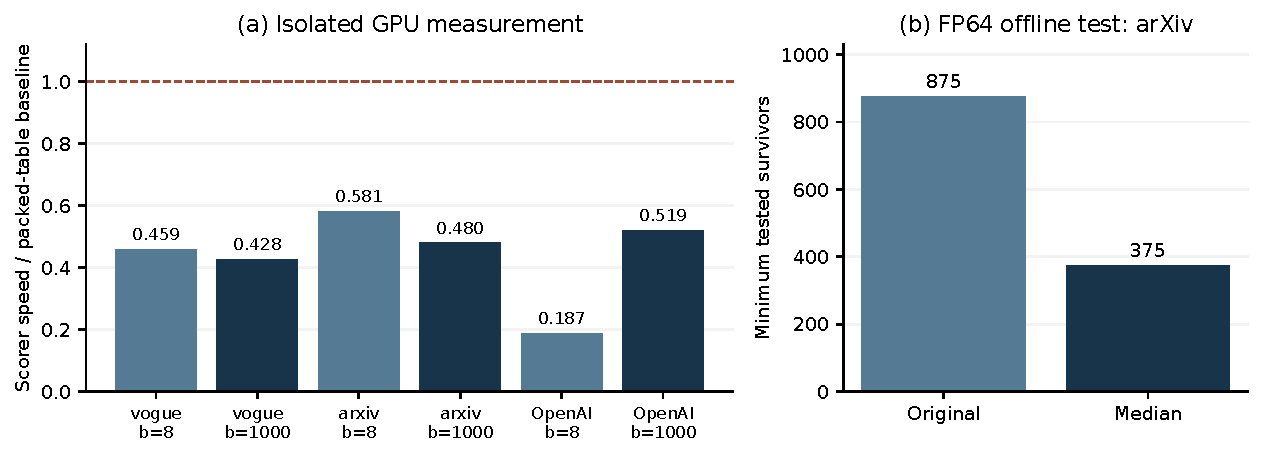
\includegraphics[width=\linewidth]{ch8/negative-evidence.pdf}
\captionof{figure}[Mailman 与面向排名的编码]{两个不同的证据边界。左：RTX 5090 上，Vogue、arXiv 和 OpenAI-3072、两个 batch、128 probes 时，最佳实测 Mailman 评分器／打包表评分器速度比，全部小于一。右：arXiv 400 查询 FP64 离线测试划分上，达到原 JHQ 召回目标的最小保留数。候选减少不是 GPU 加速。}
\label{fig:8-negative}
\end{minipage}\par\medskip

\subsection{面向排名的编码：局部收益不等于通用替代}
\label{sec:8-rank}

FP64 候选重放使用 400/200/400 个校准／\allowbreak{}验证／\allowbreak{}测试查询，测试加权分数、中位数／列表阈值、学习式损失和线性 MMSE 解码。更低 MSE 可能恶化近邻顺序；主码等级变化也会移动残差参考点。

中位阈值将 arXiv 达标的最小已测保留数从 875$\to$375，但另两个工作负载失败。对正交 $\Pi$，
\[
 \bar y=\frac1N\sum_i\Pi x_i=\Pi\bar x,
 \qquad \|\bar y\|^2=\bar x^\top\Pi^\top\Pi\bar x=\|\bar x\|^2.
\]
因此旋转保持均值向量范数，而不消除偏置。中心化也必须保持精排分数上限。

中位等级 GPU 后续实验重新训练残差。对 arXiv 原 $\alpha=100$ 目标，batch 8/1,000 下提升 $1.40/1.21\times$；Vogue 仅达到 0.9630，低于 0.9644；OpenAI-3072 持平。三轮使用独立状态／查询，不属于 E1。


\par\noindent\begin{minipage}{\linewidth}
\setlength{\parindent}{2em}
\section{内部与外部有效性的威胁}
\label{sec:8-3}
\Cref{tab:8-threats} 列出主要解释可能失效的原因以及对应对照。测量定义仍见第 3 章；重复构建和精度检查见 \cref{sec:7-8}。

\par\medskip\noindent\begin{minipage}{\linewidth}
\centering\captionsetup{hypcap=false}
\captionof{table}[有效性威胁]{有效性威胁与剩余检查。}
\label{tab:8-threats}
\footnotesize\setlength{\tabcolsep}{4pt}
\begin{tabularx}{\linewidth}{@{}*{3}{>{\raggedright\arraybackslash}X}@{}}
\toprule
受威胁主张 & 替代解释 & 对照与剩余测试 \\
\midrule
执行收益 & 分数、并列或索引状态改变造成表观收益 & CPU 重排序与表分数检查；覆盖有限，进一步测试需重新生成候选数组 \\
预算质量 & 校准样本遗漏困难查询，或工作负载改变 & 独立的带标签测试查询、已记录决策曲线和全池枚举；仍有未测查询子集与未来分布 \\
竞争优势 & 参数网格、慢调用或接口开销改变排序 & 两种召回估计器、保留慢调用、int8 与精度检查、小 batch 比较；其他设备未测 \\
容量／构建主张 & 短生命周期分配逃过峰值采样 & 分配生命周期、重复冷建和 20\,ms 显存采样；更短峰值及完整重训练前沿仍未测 \\
\bottomrule
\end{tabularx}
\end{minipage}\par\medskip

\cref{sec:7-cpu} 中较早的 CPU 比较给出了历史实现在相同召回率下的吞吐差异。独立训练、OpenAI 数据集的列表数不等以及 CPU 计时重复较少，限制了这些比值的解释。针对本文评测 GPU 版本、匹配索引和计时条件的比较仍未完成。

六个数据集不代表六种独立用户工作负载。两个 OpenAI 导出共享 DBpedia 语料，Stella 的查询从语料中留出，而非原始查询集（\cref{sec:3-2}）。比较包含传输与主机接口；内存类型及 C++ 与 Python 调用成本的差异可能影响小 batch 的小幅差距，因此不能全部归因于 GPU 搜索内核（\cref{sec:3-3}）。证据覆盖一张 GPU、静态索引和平方 L2 top-10 搜索。可能仍有近重复，并且缺少相关性标签；更新、并发服务、漂移、十亿规模容量和多 GPU 均未评估。

\end{minipage}\par

\section{未来研究方向}
\label{sec:8-4}
\subsection{考虑均值的表示}

中心化结果提示，应研究主码符号何时应编码相对均值的偏差（\cref{sec:8-centring}）。首先需要对中心化和未中心化数据重复冷建，以区分其效果与训练波动。列表相关的均值也是候选方向，但要求查询评分与残差重建保持一致。测试应比较短名单覆盖率、可达到的最佳精排召回率、所选预算和总吞吐，防止较便宜的短名单掩盖质量上限下降。

\subsection{校准风险与复用成本}

具有统计控制的预算选择，能否省下比获取预算更大的查询时间？在 \cref{eq:6-rank-curve} 的嵌套条件下，参考近邻的主码排名可代替反复试搜。早期四配置离线回放发现，序贯抽样增加了搜索次数；用已测校准时间拟合的模型估算，即使样本更少，成本仍然更高。这不是完整 GPU 控制器的测量。替代方案应测试批量试验或排名复用，并以直接校准加复用总时间，对比质量匹配的固定预算。风险分析必须覆盖抽样和预算选择程序，发生漂移时应更新校准；相对参考的控制仍需与标签建立联系，才能给出绝对召回保证。

\subsection{GPU 与主机内存间的残差存储}

BGE 和 Stella 的残差占进程总常驻显存的 80.7--82.9\%（\cref{sec:7-7}），但只有短名单中的行需要读取。将路由和主码留在 GPU，按块从主机内存取回残差，有望增加容量。难点在于把分散的短名单位置转成高效块传输。在评分与选择固定时，改变设备容量上限，测量额外字节、缓存命中、传输重叠、吞吐和尾延迟。由此才能确定容量与延迟的取舍，而非假定卸载会提高速度。

\subsection{解释小 batch 的边界}

在召回率 0.97 处，分组改善了 JHQ 的小 batch 执行，却没有消除与 CAGRA fp32 的差距（\cref{sec:7-smallbatch}）。候选工作量、选择开销和接口成本都可能参与其中。匹配的研究应统计两种索引评分的候选数，并区分内核时间、传输和主机调用开销。跨 batch 比较这些成本，才能检验下一步应减少已探测候选、降低选择成本，还是使用不同索引。


\section{部署建议}
\label{sec:8-5}
已测结果使 JHQ-GPU 成为显存受限、召回率接近 0.97 的批吞吐工作负载的候选（\cref{sec:7-2,sec:7-7}）。这不代表到该召回率之前都占优：压缩基线在部分低召回区间获胜，CAGRA fp32 则在 batch 为 8、召回率为 0.97 时获胜。对于稳定工作负载，已测的 500 查询校准可作为初始设置，随后独立核查质量，并与固定预算比较复用总时间。索引或查询分布改变后，需要重新验证。


\chapter{结论}
\label{ch:conclusion}

\section{对四个研究问题的回答}
\label{sec:9-1}

\paragraph{RQ1：GPU 索引构建与容量。}
完整 JHQ 索引能够在单张 GPU 上构建和搜索，无须把原始数据库向量保存在设备上。训练和编码均在 GPU 执行，通过有界批处理与两遍构建控制临时存储。Stella 的 17.78 百万个向量若以 FP32 保存，需要 67.81\,GiB；JHQ-GPU 的常驻进程占用为 20.44\,GiB，包括上下文与工作区。索引冷态构建耗时 10.54--10.65\,s，在这张 32\,GB 设备上采样到的峰值为 22.58\,GiB（\cref{sec:7-7}）。

\paragraph{RQ2：面向表示结构的执行。}
JHQ 的编码结构支持小查找表、连续读取和并行候选选择。每张 256 项主码表拆成两张 16 项表后保持实数算术分数，并在 24 个配置中的 22 个成为最快的已测表形式。编码按字打包，使扫描相邻候选的线程读取连续内存；多个线程还可以协作精排一个候选。小 batch 下，将一个查询分到多个 block 能增加有效并行度：batch 为 8 时，调度相对采用协作精排的单 block 基线获得 $2.727\times$ 吞吐。分组选择在全部 55,296 个已查查询实例中，与 CPU 对 GPU 分数严格排序的结果一致；单 block 的差异仅出现在截断边界的并列候选上（\cref{sec:7-3,sec:7-6,sec:7-strict-selection}）。

\paragraph{RQ3：工作负载级精排校准。}
无标签查询能够选出可复用且满足已测质量目标的精排预算，但样本数量会影响结果。使用全部 500 条校准查询时，十二个配置的留出集召回率与已测预算中最高召回率的差距均在 $10^{-3}$ 以内，最大观测损失为 0.0006。小样本可能漏掉需要更多精排的查询：采用 128 条查询时，arXiv 在 128 probes 下有 64 次抽样中的 40 次超出目标，在 512 probes 下为 64 次中的 32 次。采用 128 查询校准时，OpenAI 直接复用测试相对固定预算对照在 4--9 个 batch 内收回开销。arXiv 选出的预算则需要花更多时间来达到质量目标（\cref{sec:7-5}）。

\paragraph{RQ4：跨系统搜索性能。}
主比较显示 JHQ-GPU 适合大 batch 吞吐场景。在召回率 0.97、batch 为 1,000 时，它在四个数据集上达到 CAGRA fp32 的 $1.32$--$1.75\times$ 吞吐；在已测网格中，扣除 CUDA 上下文后的净进程显存为 CAGRA 索引分配量的 0.29--0.39。它在 Vogue 和两个 OpenAI 数据集上领先已测方法，在 arXiv 上与 IVF-RaBitQ 接近持平；Vogue 的领先依赖分组扫描（\cref{sec:7-2}）。OpenAI 测量使用 TF32 乘法；复用相同训练模型的 FP32 检查仍领先 CAGRA fp32（\cref{sec:b-precision-anchors}）。这一优势受到 batch 大小限制：batch 为 8、召回率为 0.97 时，CAGRA fp32 在四个数据集上均更快（\cref{sec:7-smallbatch}）。

\section{贡献、局限与展望}
\label{sec:9-2}

当执行方式使编码访问成本降低、并行度匹配 batch、精排满足工作负载的质量需求时，压缩才能带来容量和速度收益。

证据覆盖一张 GPU、六个准备后的数据集、平方 L2 top-10 搜索和静态索引。历史 CPU 比较不能量化本文评测版本的加速比（\cref{sec:7-cpu}）。在校准池上与参考结果一致，也仍不能确定未来查询的质量。

由此可以继续研究两个方向。风险受控的校准应考虑工作负载漂移和预计复用次数，并与质量匹配的固定预算比较包含校准开销的总时间。从主机内存取回残差码有望增加容量；测量传输量、传输与计算的重叠以及尾延迟，可判断增加容量的代价是否值得（\cref{sec:8-4}）。


\clearpage
\bibliographystyle{plainnat}
\bibliography{references}

\end{document}
